\documentclass[compress]{beamer}
\usepackage{ifthen,verbatim}

\newcommand{\isnote}{}
\xdefinecolor{lightyellow}{rgb}{1.,1.,0.25}
\xdefinecolor{darkblue}{rgb}{0.1,0.1,0.7}

%% Uncomment this to get annotations
%% \def\notes{\addtocounter{page}{-1}
%%            \renewcommand{\isnote}{*}
%% 	   \beamertemplateshadingbackground{lightyellow}{white}
%%            \begin{frame}
%%            \frametitle{Notes for the previous page (page \insertpagenumber)}
%%            \itemize}
%% \def\endnotes{\enditemize
%% 	      \end{frame}
%%               \beamertemplateshadingbackground{white}{white}
%%               \renewcommand{\isnote}{}}

%% Uncomment this to not get annotations
\def\notes{\comment}
\def\endnotes{\endcomment}

\setbeamertemplate{navigation symbols}{}
\setbeamertemplate{headline}{\mbox{ } \hfill
\begin{minipage}{5.5 cm}
\vspace{-0.75 cm} \small
\end{minipage} \hfill
\begin{minipage}{4.5 cm}
\vspace{-0.75 cm} \small
\begin{flushright}
\ifthenelse{\equal{\insertpagenumber}{1}}{}{Jim Pivarski \hspace{0.2 cm} \insertpagenumber\isnote/\pageref{numpages}}
\end{flushright}
\end{minipage}\mbox{\hspace{0.2 cm}}\includegraphics[height=1 cm]{../cmslogo} \hspace{0.1 cm} \includegraphics[height=1 cm]{../tamulogo} \hspace{0.01 cm} \vspace{-1.05 cm}}

\begin{document}
\begin{frame}
\vfill
\begin{center}
\textcolor{darkblue}{\Large Plans and Prior Work on Muon Jets}

\vfill
\begin{columns}
\column{0.3\linewidth}
\begin{center}
\large
\textcolor{darkblue}{\it Jim Pivarski}

Aysen Tatarinov

Alexei Safonov
\end{center}
\end{columns}

\begin{columns}
\column{0.3\linewidth}
\begin{center}
\scriptsize
{\it Texas A\&M University}
\end{center}
\end{columns}

\vfill
11 May, 2010

\end{center}
\end{frame}

%% \begin{notes}
%% \item This is the annotated version of my talk.
%% \item If you want the version that I am presenting, download the one
%% labeled ``slides'' on Indico (or just ignore these yellow pages).
%% \item The annotated version is provided for extra detail and a written
%% record of comments that I intend to make orally.
%% \item Yellow notes refer to the content on the {\it previous} page.
%% \item All other slides are identical for the two versions.
%% \end{notes}

\small

\begin{frame}
\frametitle{Proposed search strategy}
\begin{itemize}
\item The theoretical motivation for lepton jets is a broad idea,
  rather than a specific model, so we want to keep our search general
\item This is common problem: model-specific searches are limiting,
  but unspecific searches are not well defined--- how do we look for
  ``anything interesting''?  How to balance definiteness with generality?
\item Proposal: let the backgrounds define the search; look for all
  the ways that a signal could peek out from under the Standard Model
\begin{enumerate}[(\alph{enumi}) ]
\item tightly collimated group of leptons with $N_{\mbox{\scriptsize
    leptons}} > 2$: background for $N_{\mbox{\scriptsize
    leptons}} = 2$ is large ($b \to \ell c \to \ell\ell s$) but not $N_{\mbox{\scriptsize
    leptons}} > 2$.
  Could be useful to add electrons and even pions for this kind of
  search, since the acceptance for \mbox{muons-only falls as
    $\sim\left(\frac{1}{2}\right)^{N_\mu/2}$ {\scriptsize (lepton universality)}\hspace{-1 cm}}

\vspace{0.2 cm}
\item more than one tightly collimated group of leptons (at first, only look for groups of muons, maybe add electrons later)

\vspace{0.2 cm}
\item one group of muons and large missing energy

\vspace{0.2 cm}
\item {\it muon} pair or group with significantly displaced vertex (not electrons; background from conversions)
\end{enumerate}
\end{itemize}
%% \hspace{-0.83 cm} \textcolor{darkblue}{\Large Outline2}
\end{frame}

\begin{frame}
\frametitle{Proposed search strategy}

\begin{itemize}
\item Motivations by event topology:
\begin{enumerate}[(\alph{enumi}) ]
\item \textcolor{gray}{tightly collimated group of leptons with $N_{\mbox{\scriptsize
    leptons}} > 2$: background for $N_{\mbox{\scriptsize
    leptons}} = 2$ is large ($b \to \ell c \to \ell\ell s$) but not $N_{\mbox{\scriptsize
    leptons}} > 2$.
  Could be useful to add electrons and even pions for this kind of
  search, since the acceptance for \mbox{muons-only falls as
    $\sim\left(\frac{1}{2}\right)^{N_\mu/2}$ {\scriptsize (lepton universality)}\hspace{-1 cm}}}

Cascades of new resonances, all of which are light: $a_2 \to a_1 a_1 \to 4\ell$, $a_3 \to a_2 a_2 \to 4a_1 \to 8\ell$, etc.
\vspace{0.2 cm}
\item \textcolor{gray}{more than one tightly collimated group of leptons (at first, only look for groups of muons, maybe add electrons later)}

One of the new resonances is heavy: e.g.\ NMSSM Higgs $h \to a a \to 4\ell$ with $m_h \sim 100$~GeV, $m_a \sim 2$~GeV

\vspace{0.2 cm}
\item \textcolor{gray}{one group of muons and large missing energy}

Final state radiation of a dark photon off of a WIMP

\vspace{0.2 cm}
\item \textcolor{gray}{{\it muon} pair or group with significantly displaced vertex (not electrons; background from conversions)}

New resonance with very small couplings to Standard Model particles
\end{enumerate}
\end{itemize}
\end{frame}

\begin{frame}
\frametitle{Aysen's physics interests}

\begin{itemize}
\item Aysen Tatarinov is a grad student at A\&M
\item He's specifically interested in a ``two well-separated muon jets'' topology (case \textcolor{darkblue}{(b)})
\item We published a phenomenology paper on this recently {\scriptsize (\href{http://prd.aps.org/abstract/PRD/v81/i7/e075021}{Phys. Rev. D 81, 075021 (2010)}, \href{http://arxiv.org/abs/1002.1956}{arXiv:1002.1956})}
\end{itemize}

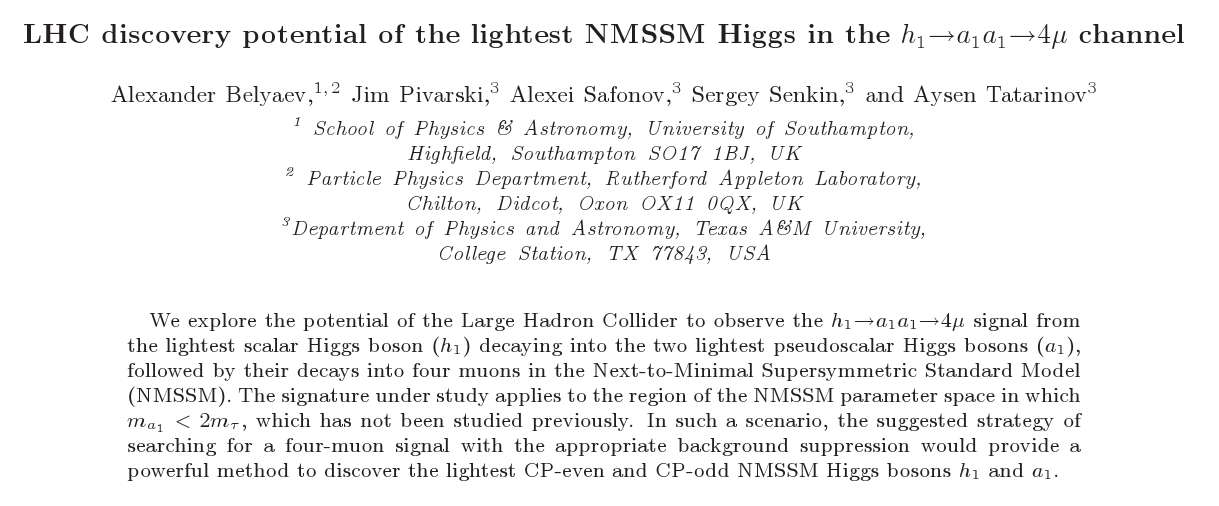
\includegraphics[width=\linewidth]{higgspaper.png}

\end{frame}

\begin{frame}
\frametitle{Quick backgrounds estimations}
\begin{itemize}
\item ``background'' = InclusiveMu15
\item ``signal'' = typical 1~pb$^{-1}$ model {\scriptsize ($\mathcal{U}(1)_{\mbox{\tiny dark}}$ with 1~GeV $Z_{\mbox{\tiny dark}}$, 3~GeV $h_{\mbox{\tiny dark}}$)}
\end{itemize}

\begin{columns}
\column{0.6\linewidth}
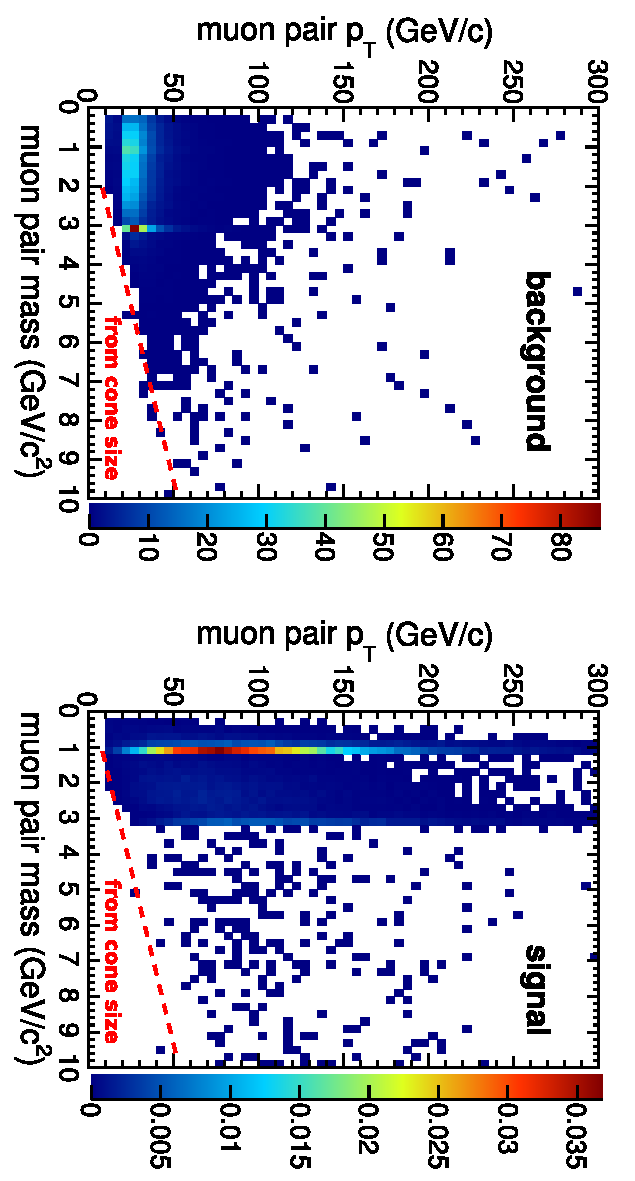
\includegraphics[height=\linewidth, angle=90]{backgrounds_basic.pdf}
\column{0.4\linewidth}
No cuts.  Color scale is cross-section per bin; note the different scales!
\end{columns}

\begin{columns}
\column{0.6\linewidth}
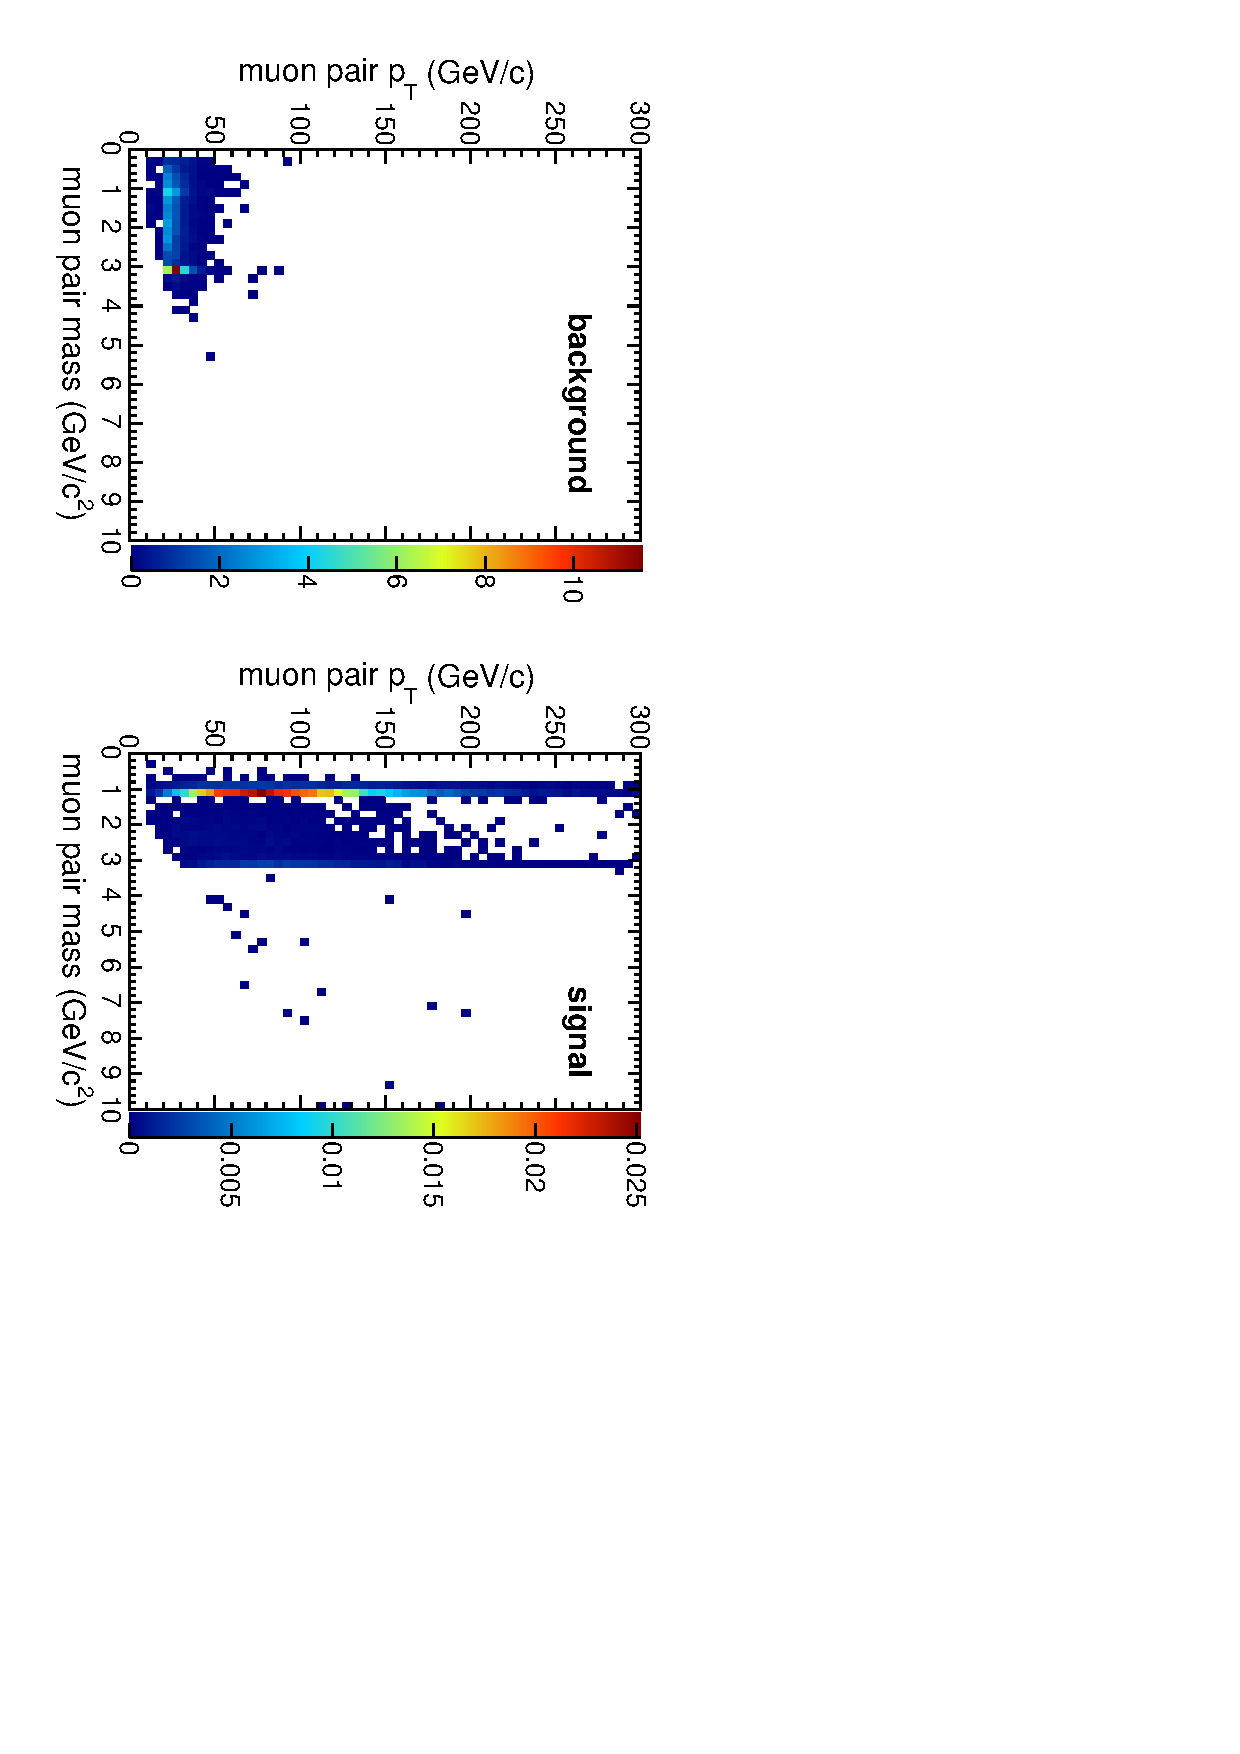
\includegraphics[height=\linewidth, angle=90]{backgrounds_jpsiiso.pdf}
\column{0.4\linewidth}
Same with a reasonable isolation cut (factor of 10 for background)
\end{columns}

%% \begin{columns}
%% \column{0.4\linewidth}
%% 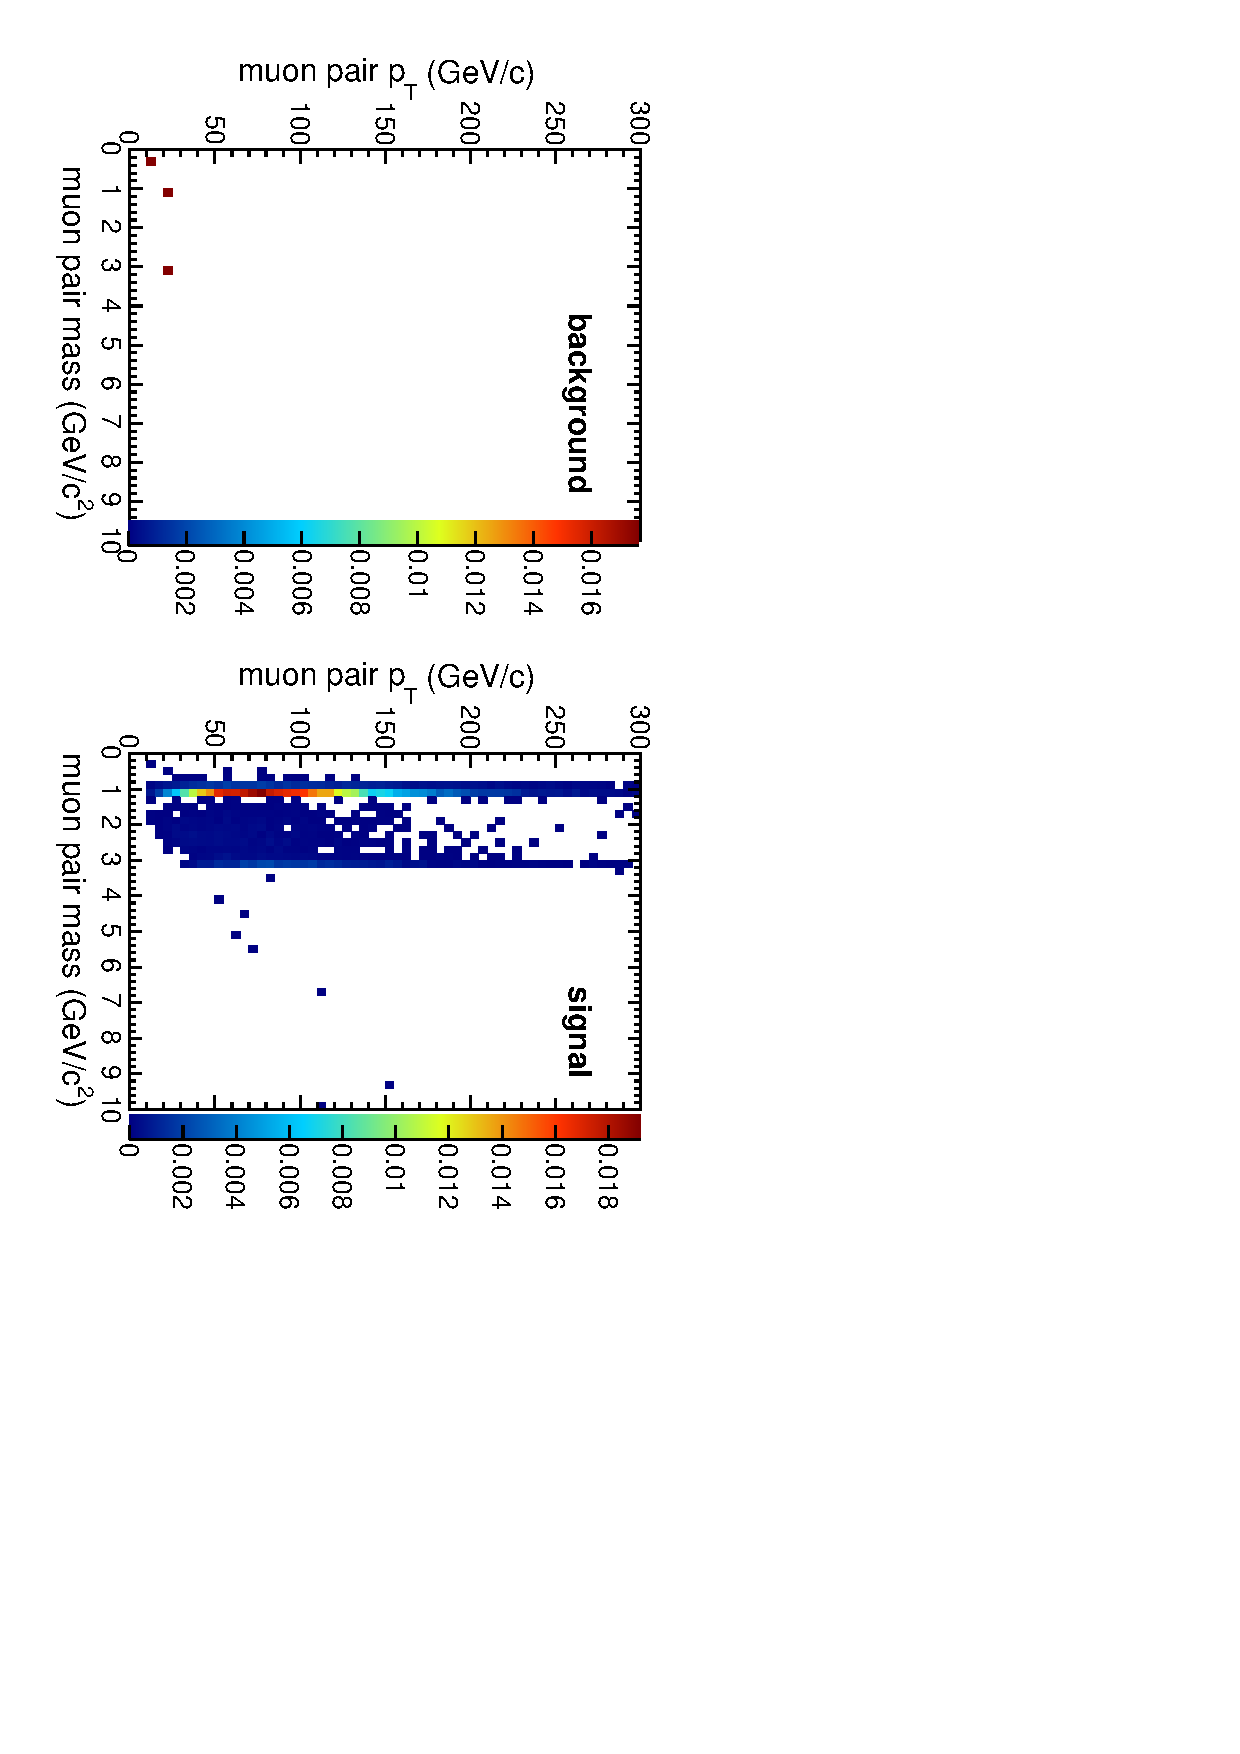
\includegraphics[height=\linewidth, angle=90]{backgrounds_jpsiisotwo.pdf}
%% \column{0.6\linewidth}
%% Isolation and $\ge 2$ distinct jets (case \textcolor{darkblue}{(b)})
%% \end{columns}
\end{frame}

\begin{frame}
\frametitle{Quick backgrounds estimations}

Vertical axis is cross-section per bin; note the different scales!

\vfill
\renewcommand{\arraystretch}{1.5}
\begin{tabular}{c c}
Motivating case \textcolor{darkblue}{(a)} & Motivating case \textcolor{darkblue}{(b)} \\
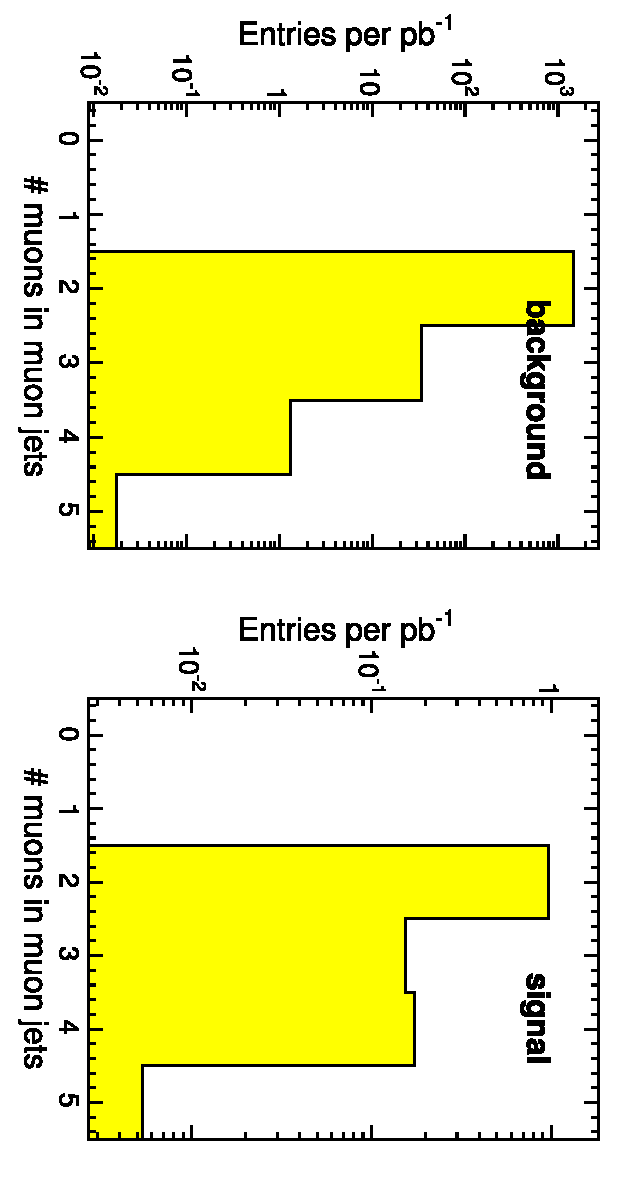
\includegraphics[height=0.45\linewidth, angle=90]{backgrounds_muonsperjet.pdf} & 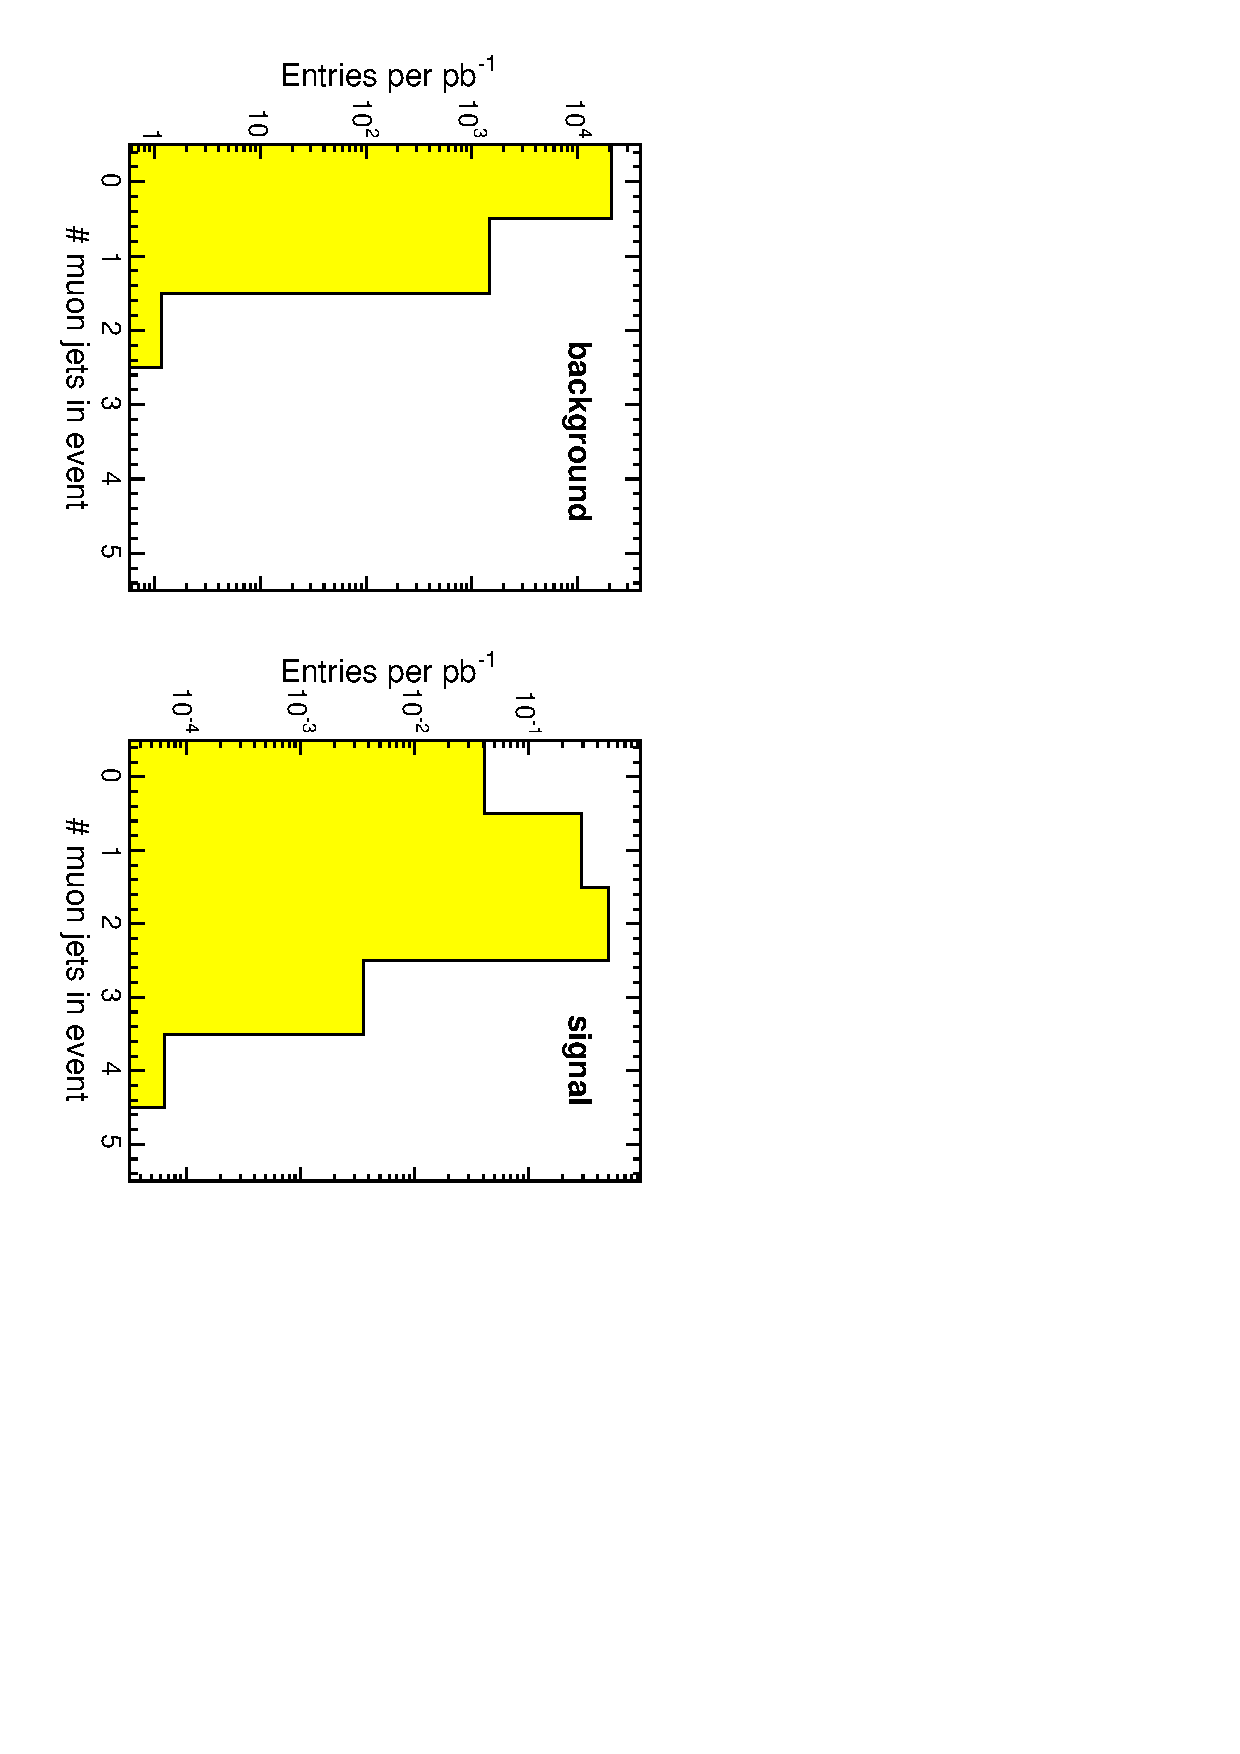
\includegraphics[height=0.45\linewidth, angle=90]{backgrounds_jetsperevent.pdf} \\
with isolation: & with isolation: \\
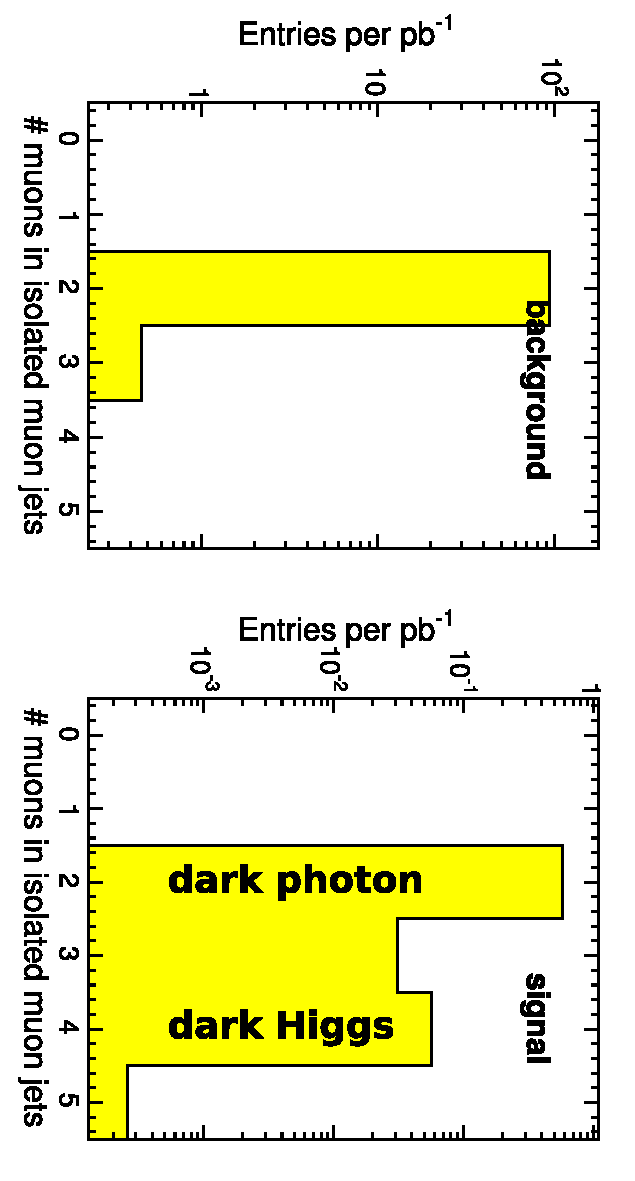
\includegraphics[height=0.45\linewidth, angle=90]{backgrounds_muonspergoodjet.pdf} & 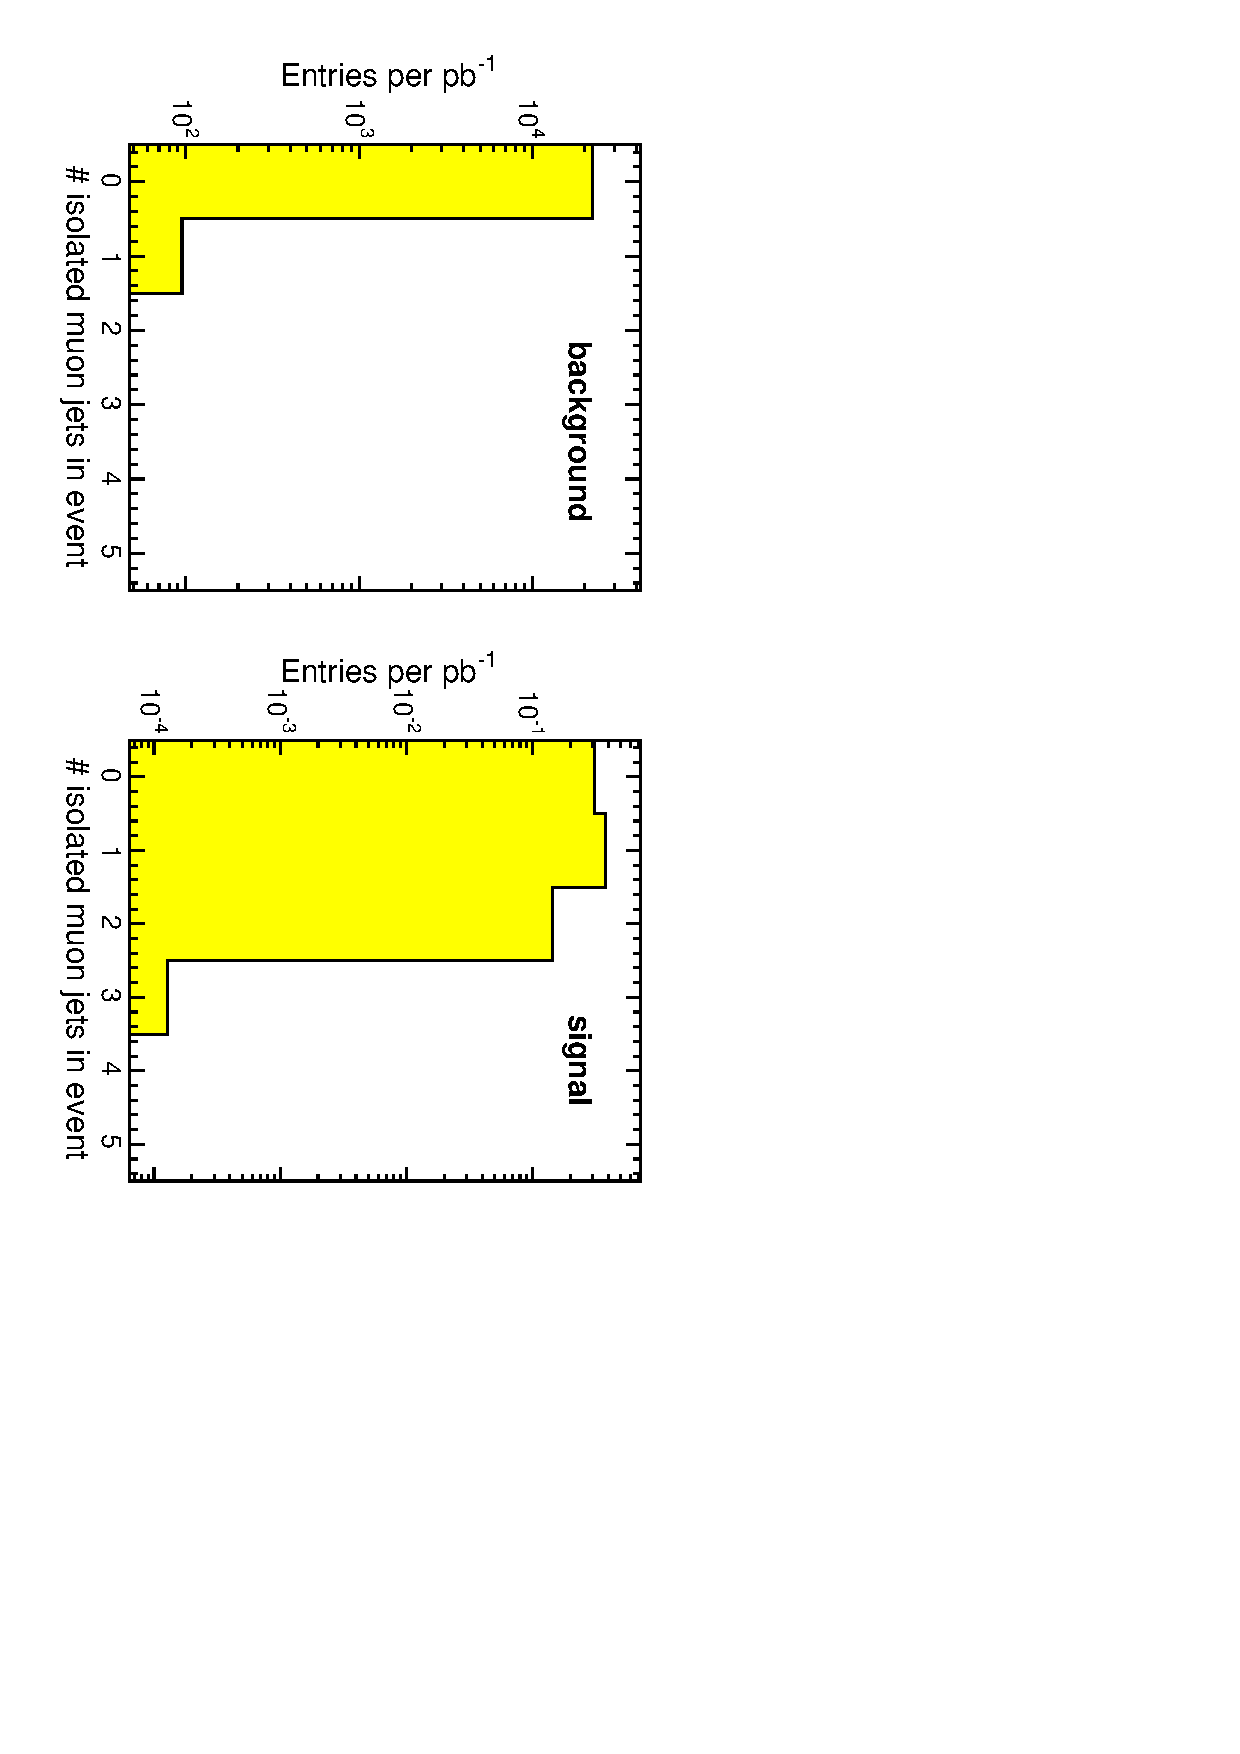
\includegraphics[height=0.45\linewidth, angle=90]{backgrounds_goodjetsperevent.pdf} \\
%% $h_{\mbox{\tiny dark}} \to Z_{\mbox{\tiny dark}}Z_{\mbox{\tiny dark}} \to 4\mu$ cascades & multi-$Z_{\mbox{\tiny dark}}$ events \\
%% at $N_{\mbox{\scriptsize muons}} = 4$ & at $N_{\mbox{\scriptsize jets}} \ge 2$ \\
\end{tabular}
\end{frame}

\begin{frame}
\frametitle{Sources of backgrounds}

\begin{itemize}
\item Physics
\begin{itemize}
\item heavy flavor double-semileptonic: continuum in mass
\item light flavor decay-in-flight: cut with vertex probability
\item quarkonium resonances: also useful as standard candles
\item Drell-Yan, diboson: weak and usually large $\Delta R$
\end{itemize}
\begin{center}
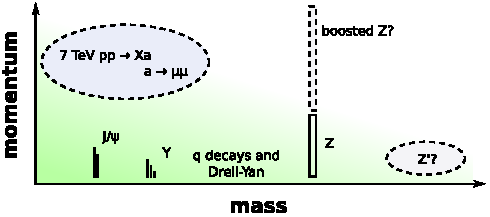
\includegraphics[width=0.7\linewidth]{where_we_live.pdf}
\end{center}

\item Misreconstruction: small number of muons misreconstructed as a
  larger number of muons
\begin{itemize}
\item similar to efficiency issues: large number of muons misreconstructed as
  a smaller number of muons
\end{itemize}
\end{itemize}
\end{frame}

\begin{frame}
\frametitle{Potentially useful datasets}

\hfill
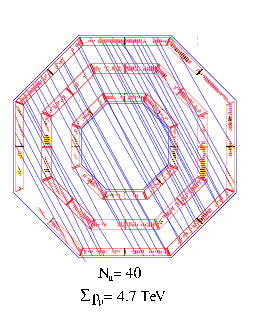
\includegraphics[height=3 cm]{airshowers_example_more_than_we_want.png}
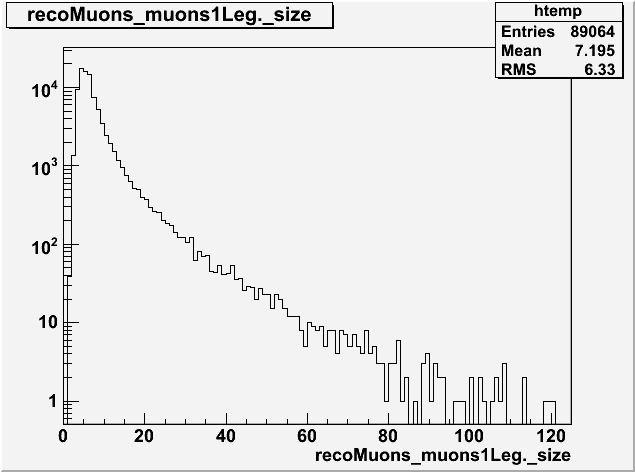
\includegraphics[height=3 cm]{airshowers_in_muon_system.png}

\vspace{-3 cm}
\begin{itemize}
\item Cosmic ray air

showers: already-

available source

of multi-muon events;

some may be close

enough to each other to study \mbox{two-muon efficiency/misreconstruction\hspace{-5 cm}}

\item High-intensity beam-halo: same argument for endcaps, assuming that the LHC beam-halo production process yields any multiple-muon events (unchecked)

\vspace{0.2 cm}
\hfill 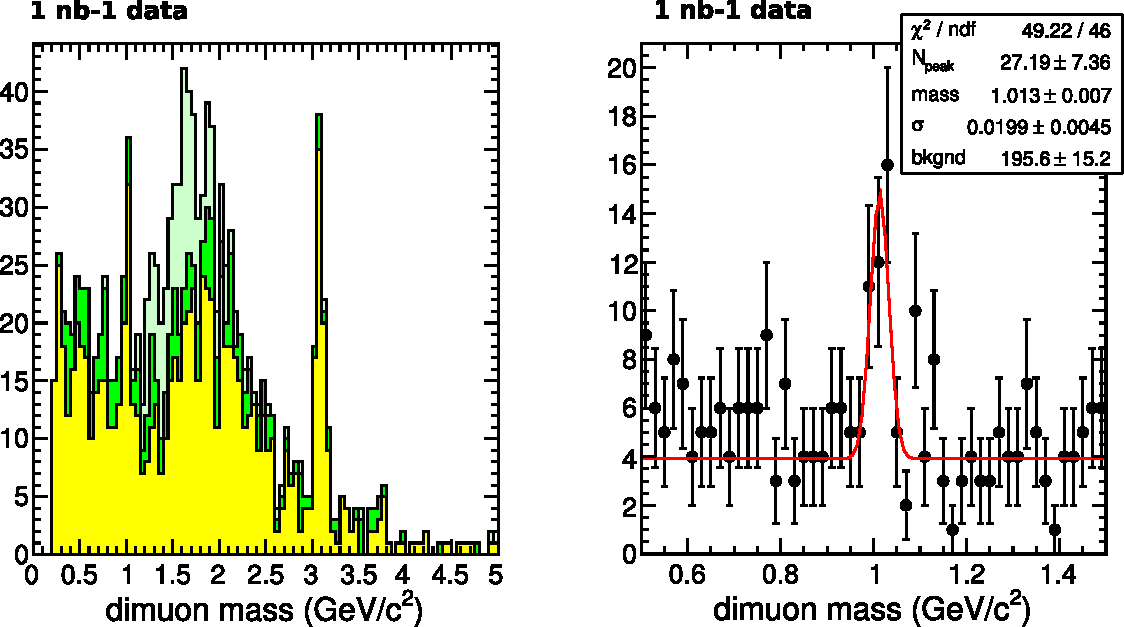
\includegraphics[height=3 cm]{real_mass_peaks.pdf}

\vspace{-3.4 cm}
\item $J/\psi$ and $\phi(1020)$ resonances:

high-momentum tail of $J/\psi$,

$\phi$ distributions are standard-

candle lepton jets--- how high

in momentum can we expect

to find them?
\end{itemize}
\end{frame}

\begin{frame}
\frametitle{Studying misreconstruction}

\begin{description}
\item[low-level:] Select nearby pairs of RPC hits or DT/CSC segments
  in cosmic air showers: look for segments in an adjacent chamber

\item[medium-level:] Identify real trackerMuon pairs with $J/\psi$
  mass cut and check standAloneMuon reconstruction efficiency

\item[high-level:] Dissect trackerMuons/standAloneMuons/globalMuons

Standard ``muons'' collection contains muons derived from all
algorithms, but each algorithm has different efficiencies and
backgrounds, especially for close-by muons
\begin{itemize}
\item trackerMuons: large backgrounds from two or more tracks matched
  to one muon's segments
\item standAloneMuons: low efficiency from reconstruction algorithm
  with nearby segments
\item globalMuons: should inherit low efficiency from standAloneMuons
\end{itemize}

Build single-algorithm collections and perform analysis independently on each
\end{description}
\end{frame}

\begin{frame}
\frametitle{Early misreconstruction studies}

Opposite-sign muon pair gun: color scale is probability of reconstructing exactly two muons {\scriptsize (no underlying event to add backgrounds to trackerMuons)}

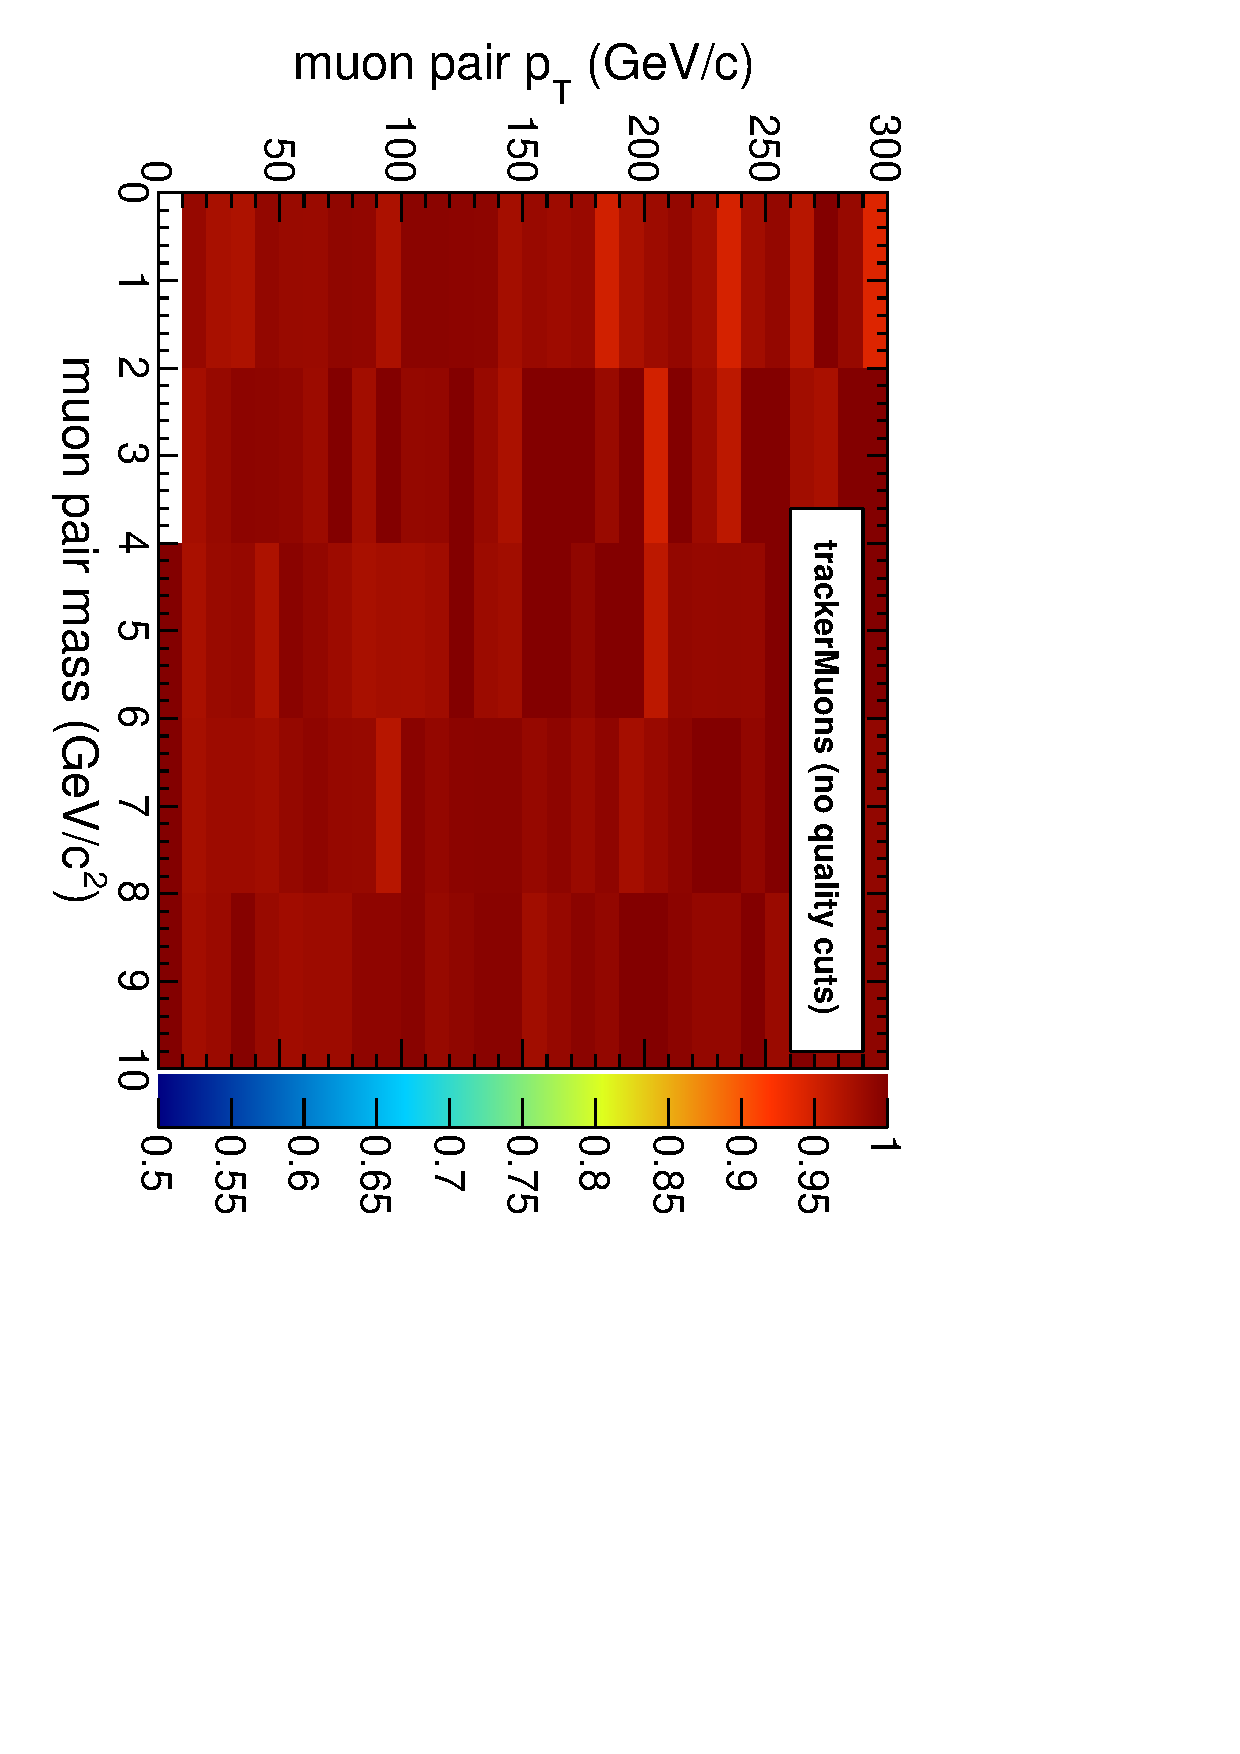
\includegraphics[height=0.5\linewidth, angle=90]{efficiency2d_tracker.pdf}
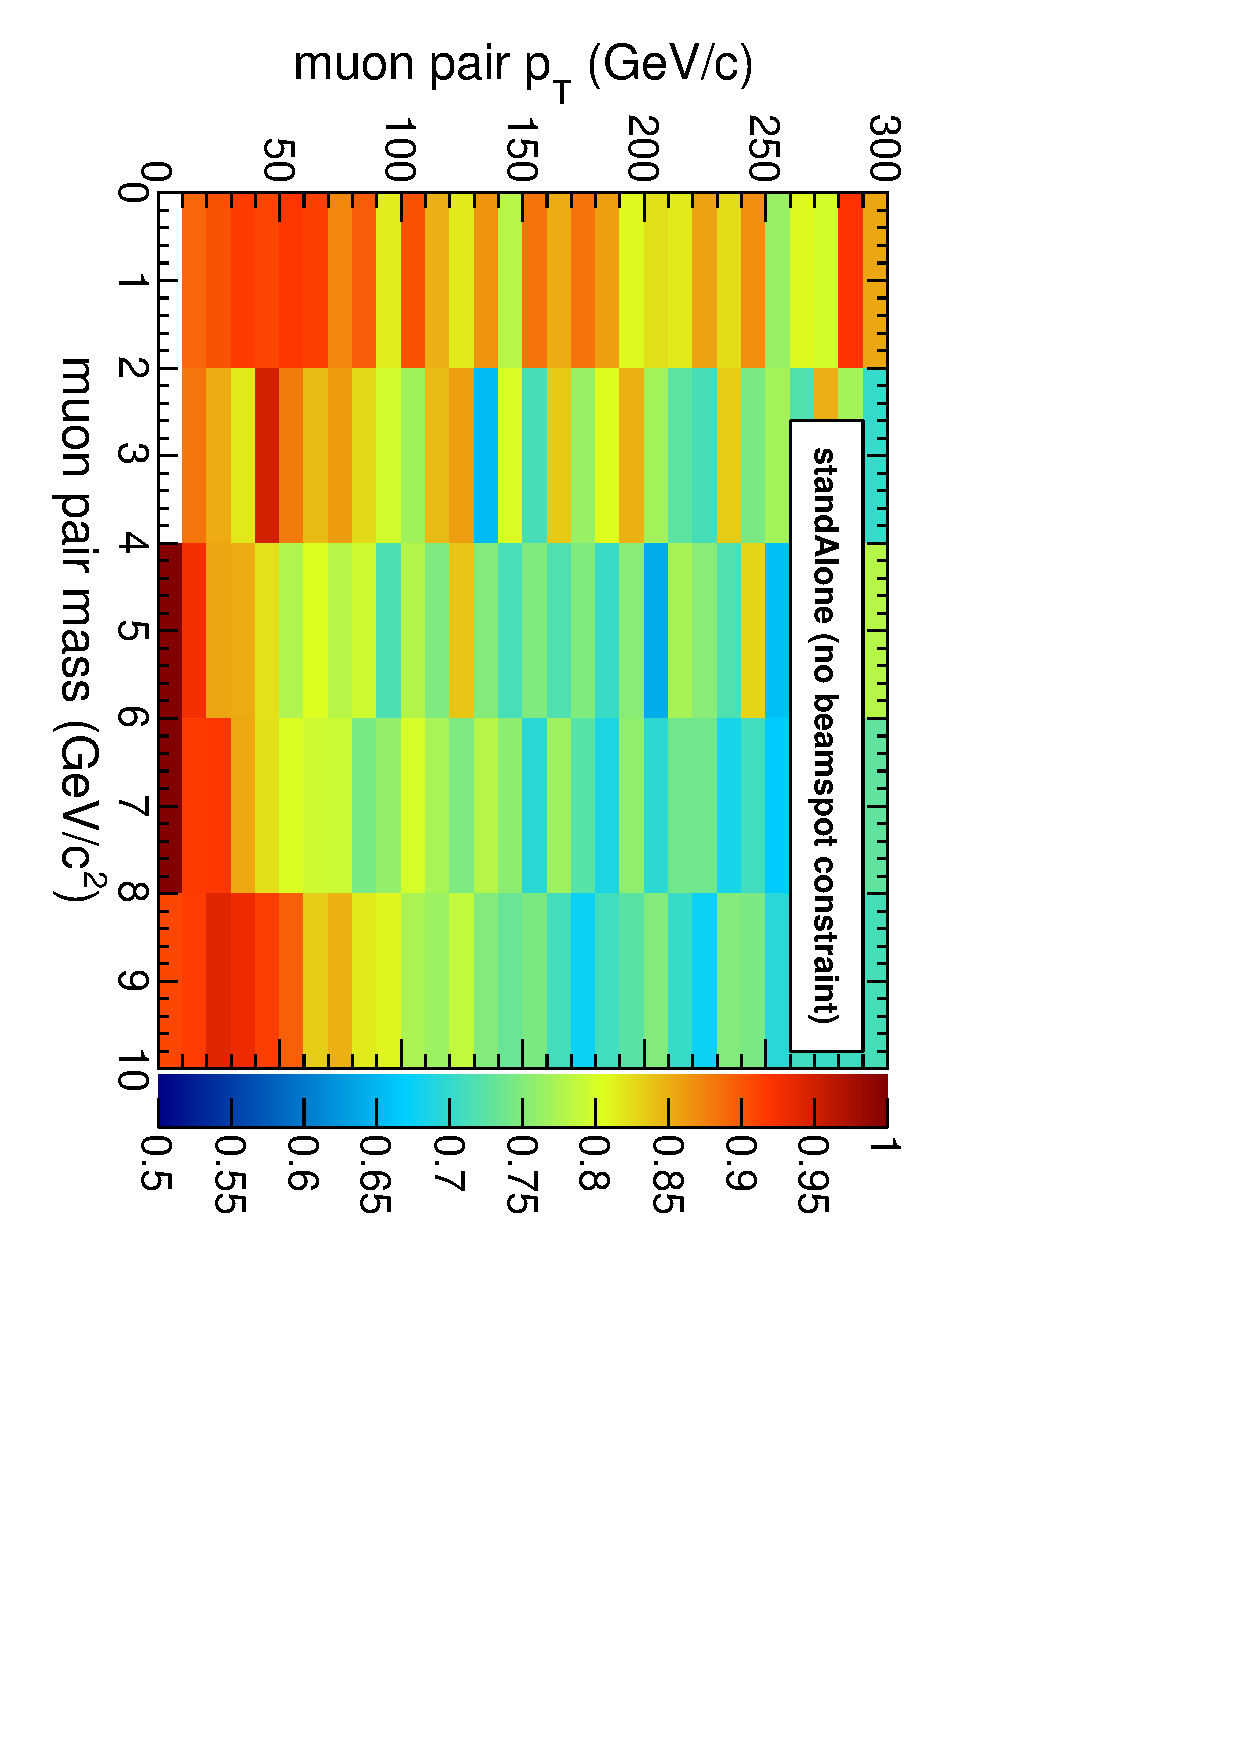
\includegraphics[height=0.5\linewidth, angle=90]{efficiency2d_stand.pdf}

\only<1>{\mbox{Directly related to how close they approach each other in muon system:\hspace{-1 cm}}}
\only<2>{\mbox{Interestingly little dependence on position in chamber (such as edges):\hspace{-1 cm}}}

\only<1>{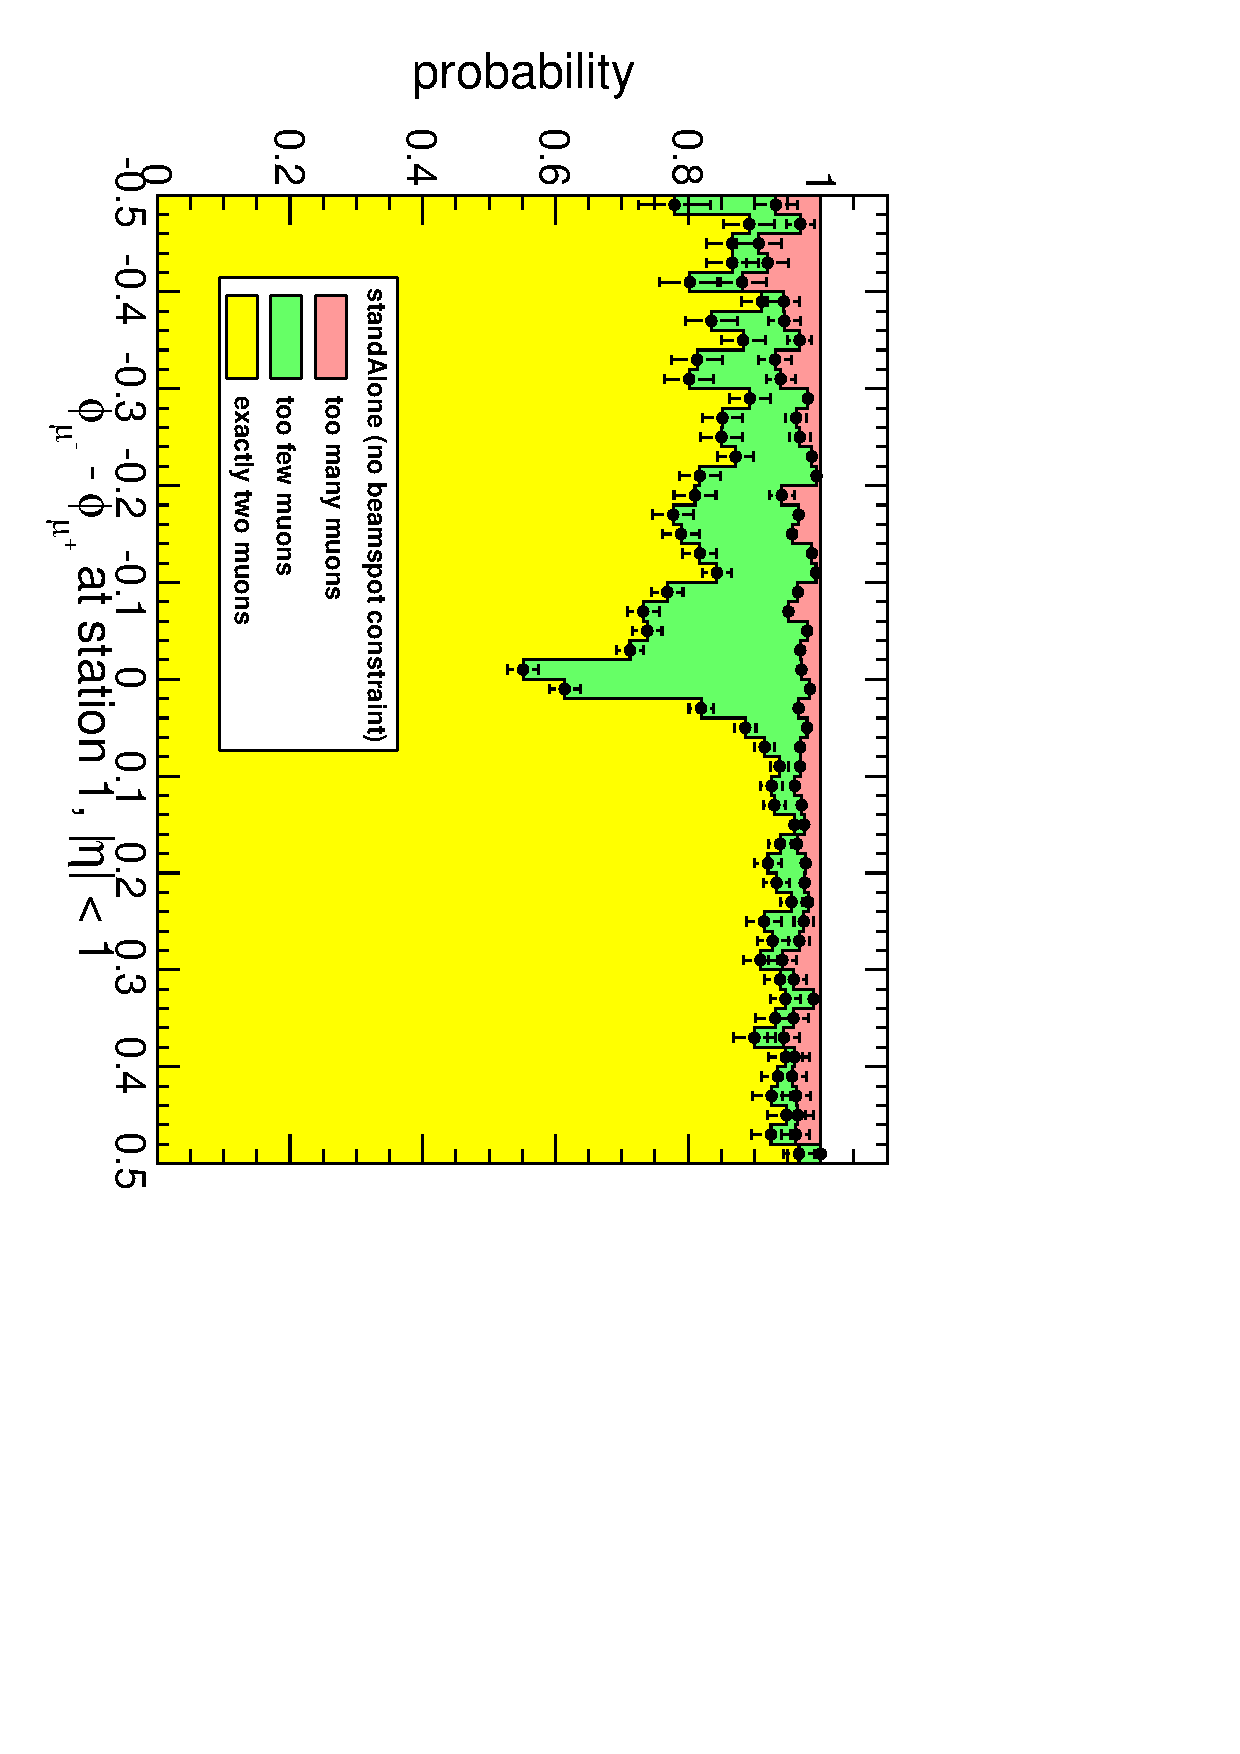
\includegraphics[height=0.33\linewidth, angle=90]{efficiency_standPhiDiff0.pdf}
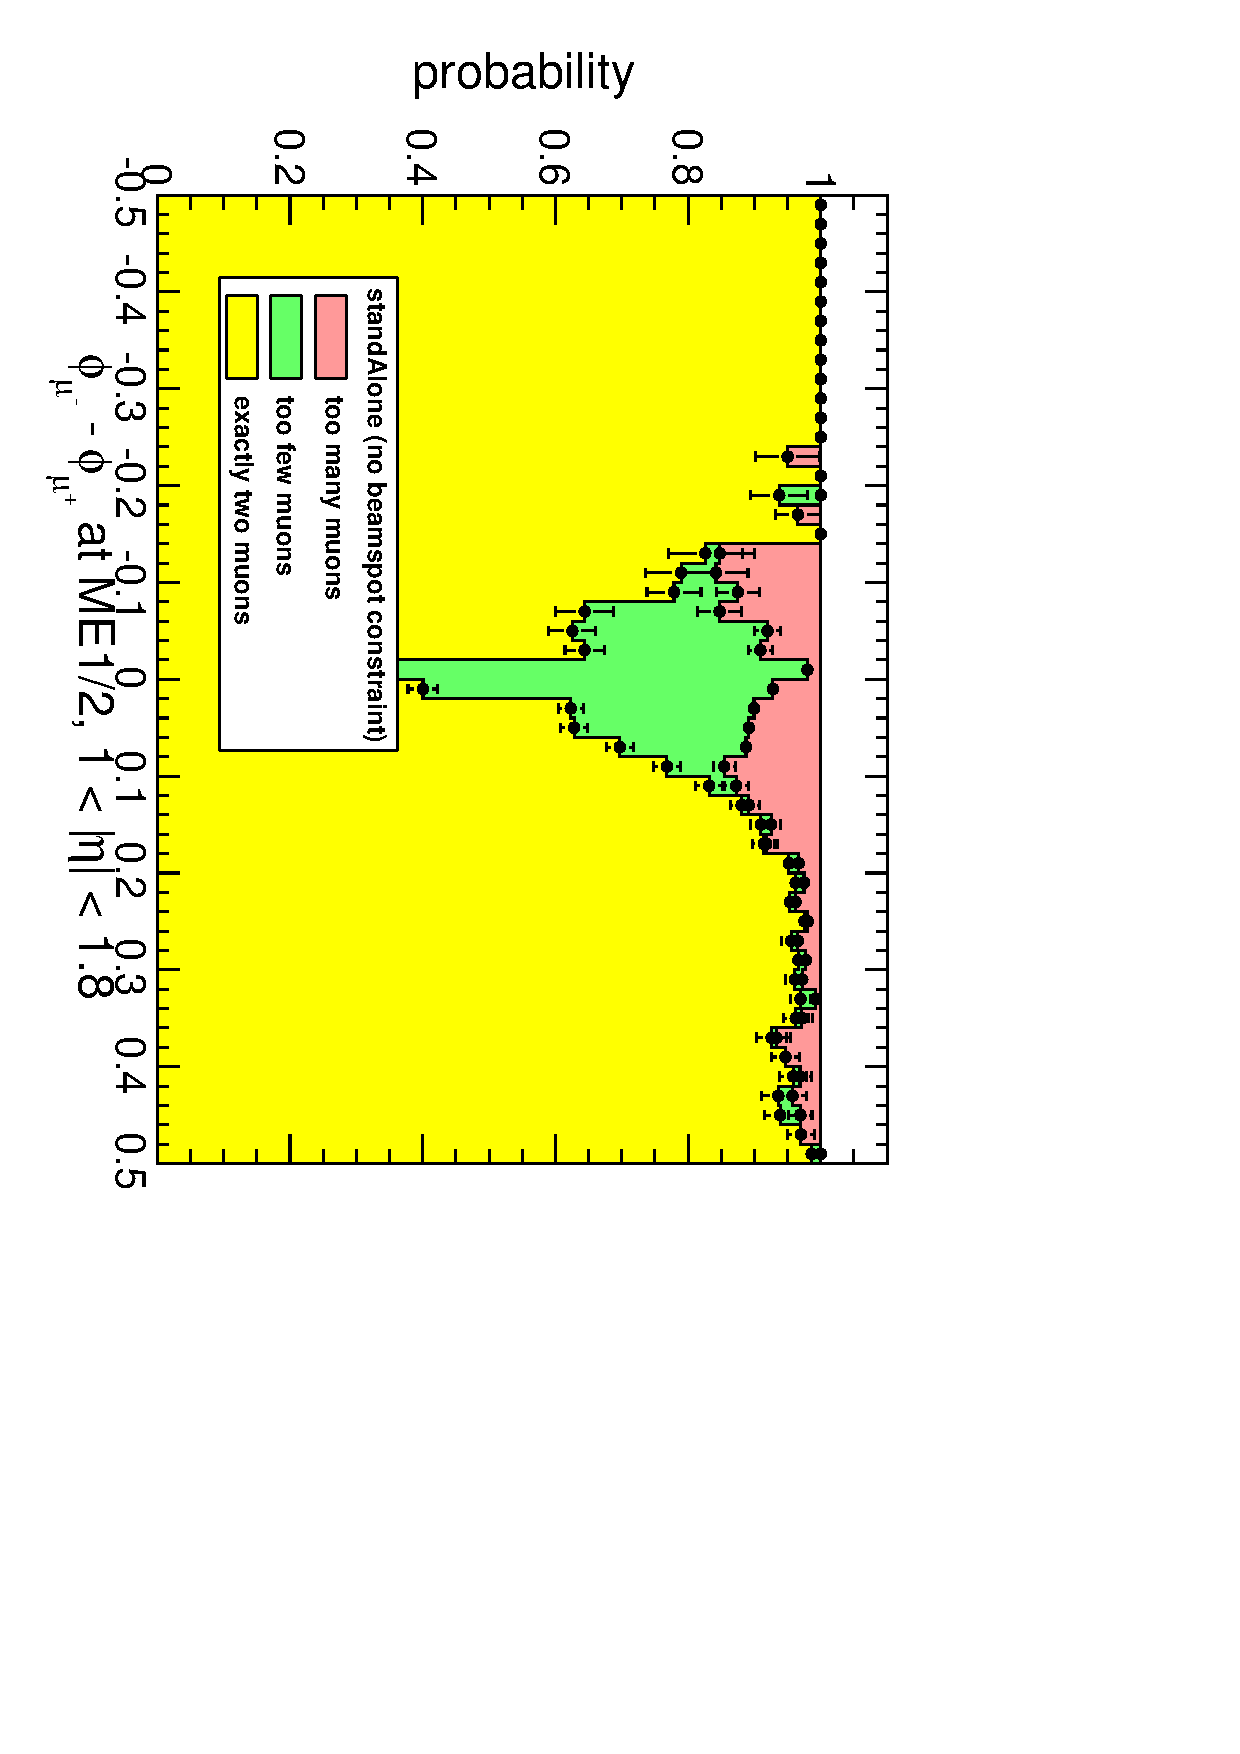
\includegraphics[height=0.33\linewidth, angle=90]{efficiency_standPhiDiff1.pdf}
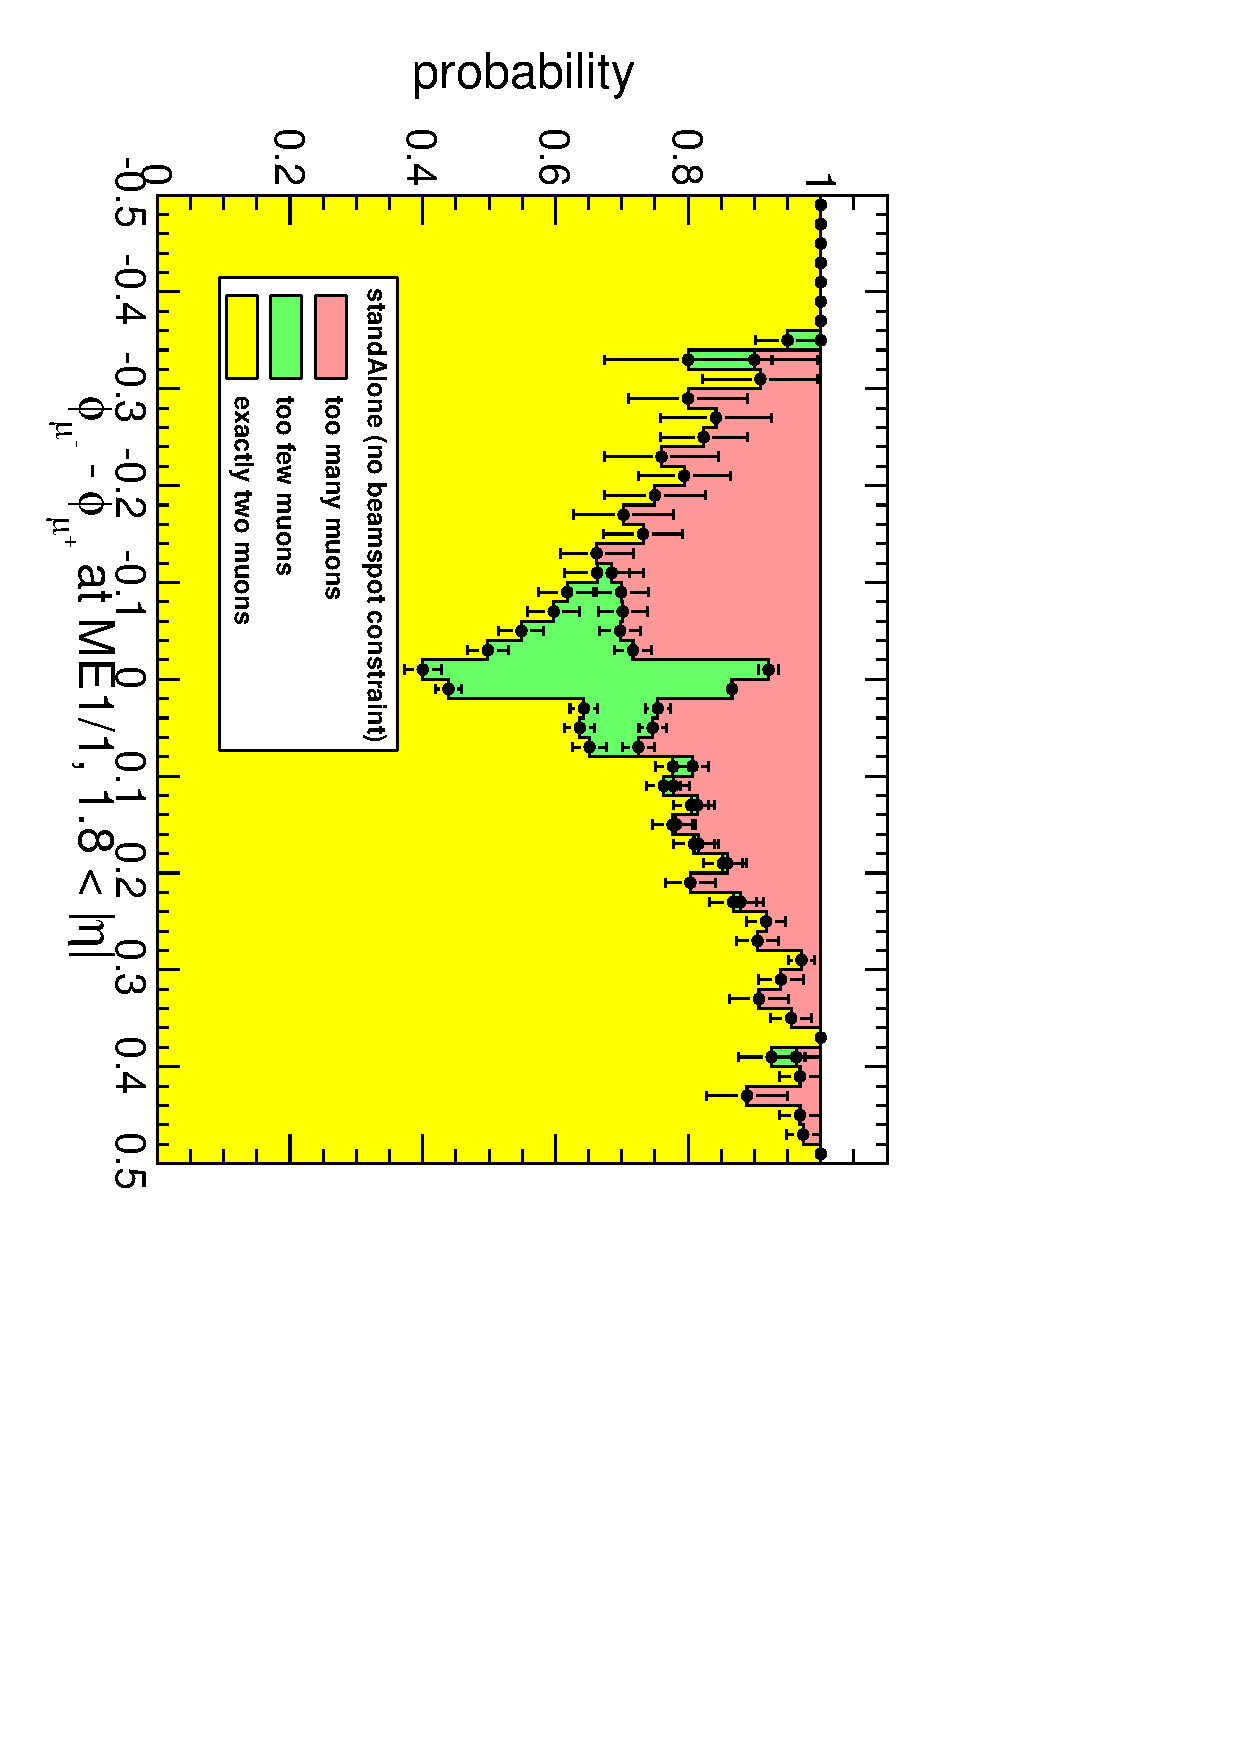
\includegraphics[height=0.33\linewidth, angle=90]{efficiency_standPhiDiff2.pdf}}
\only<2>{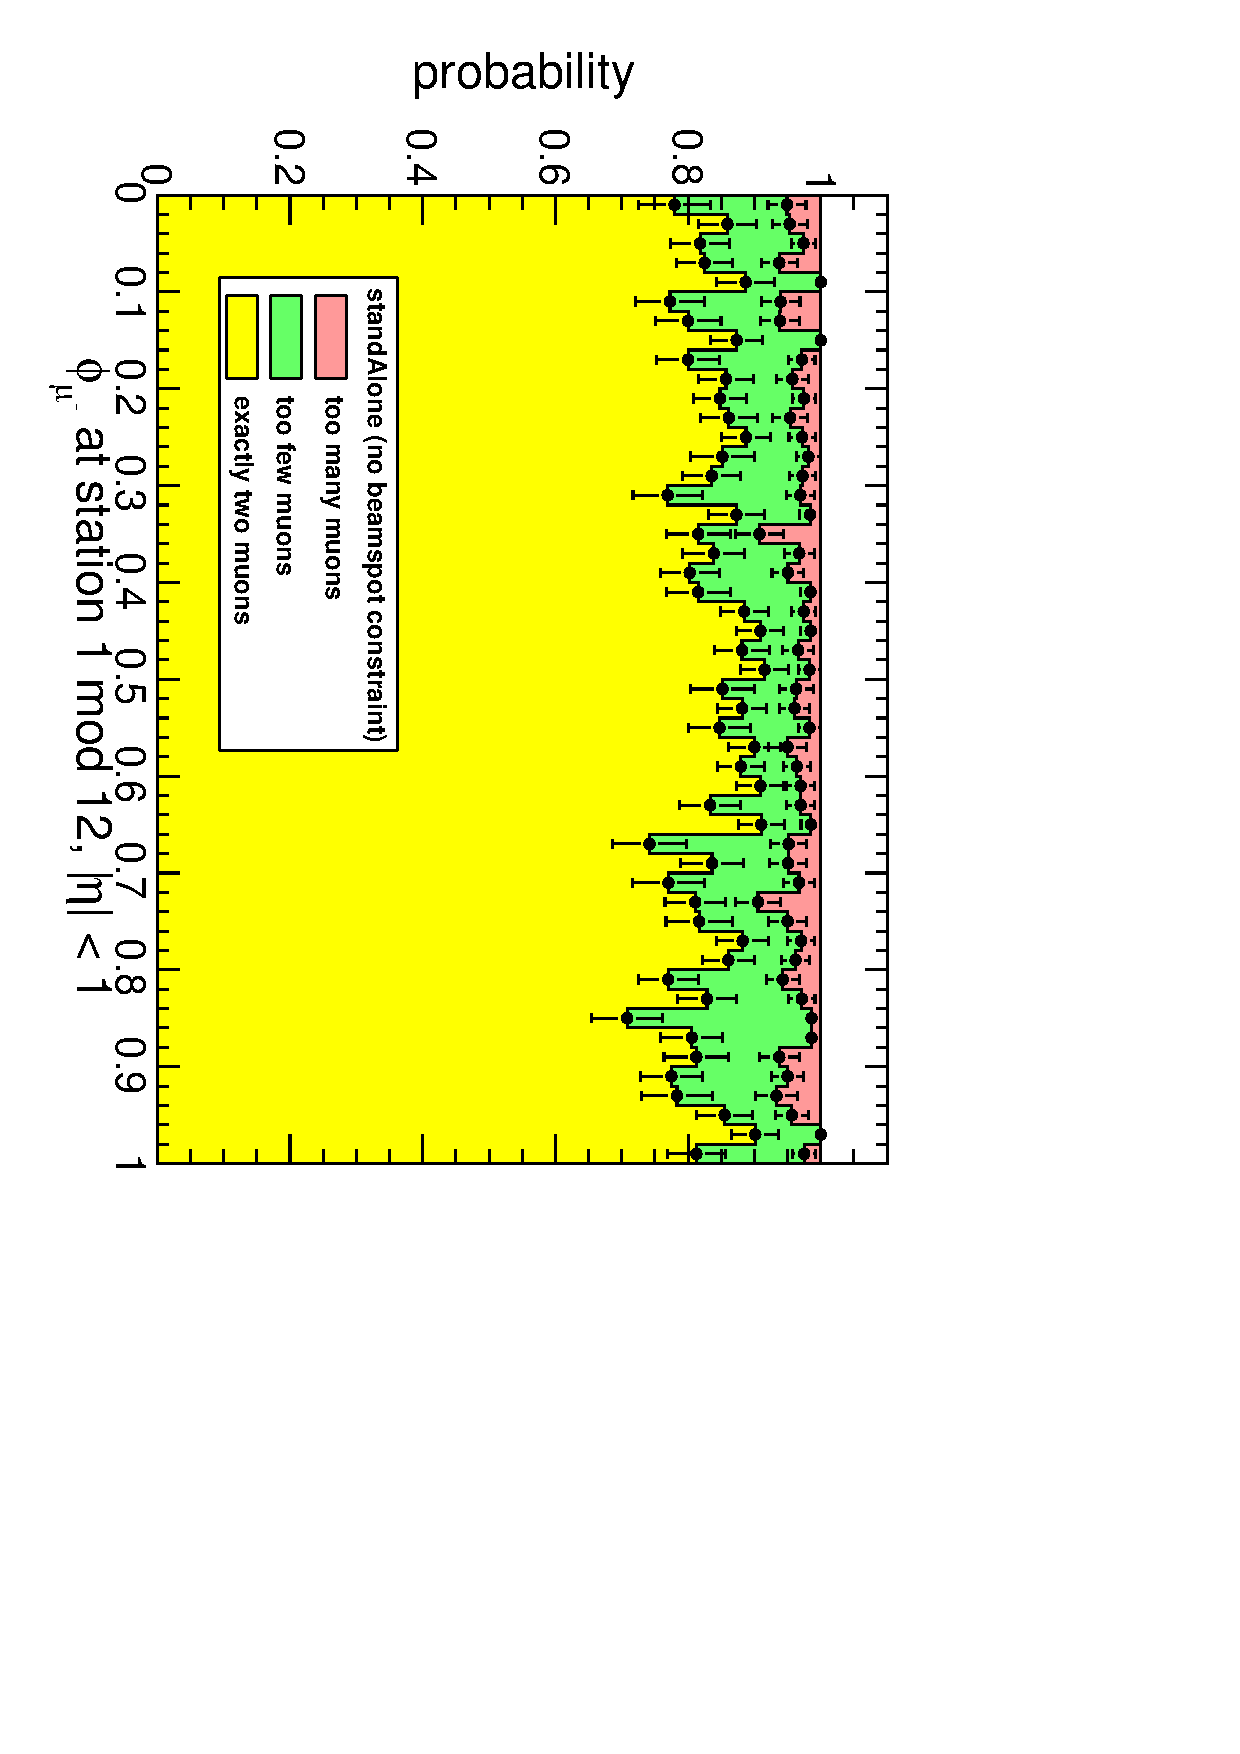
\includegraphics[height=0.33\linewidth, angle=90]{efficiency_standPhimod0.pdf}
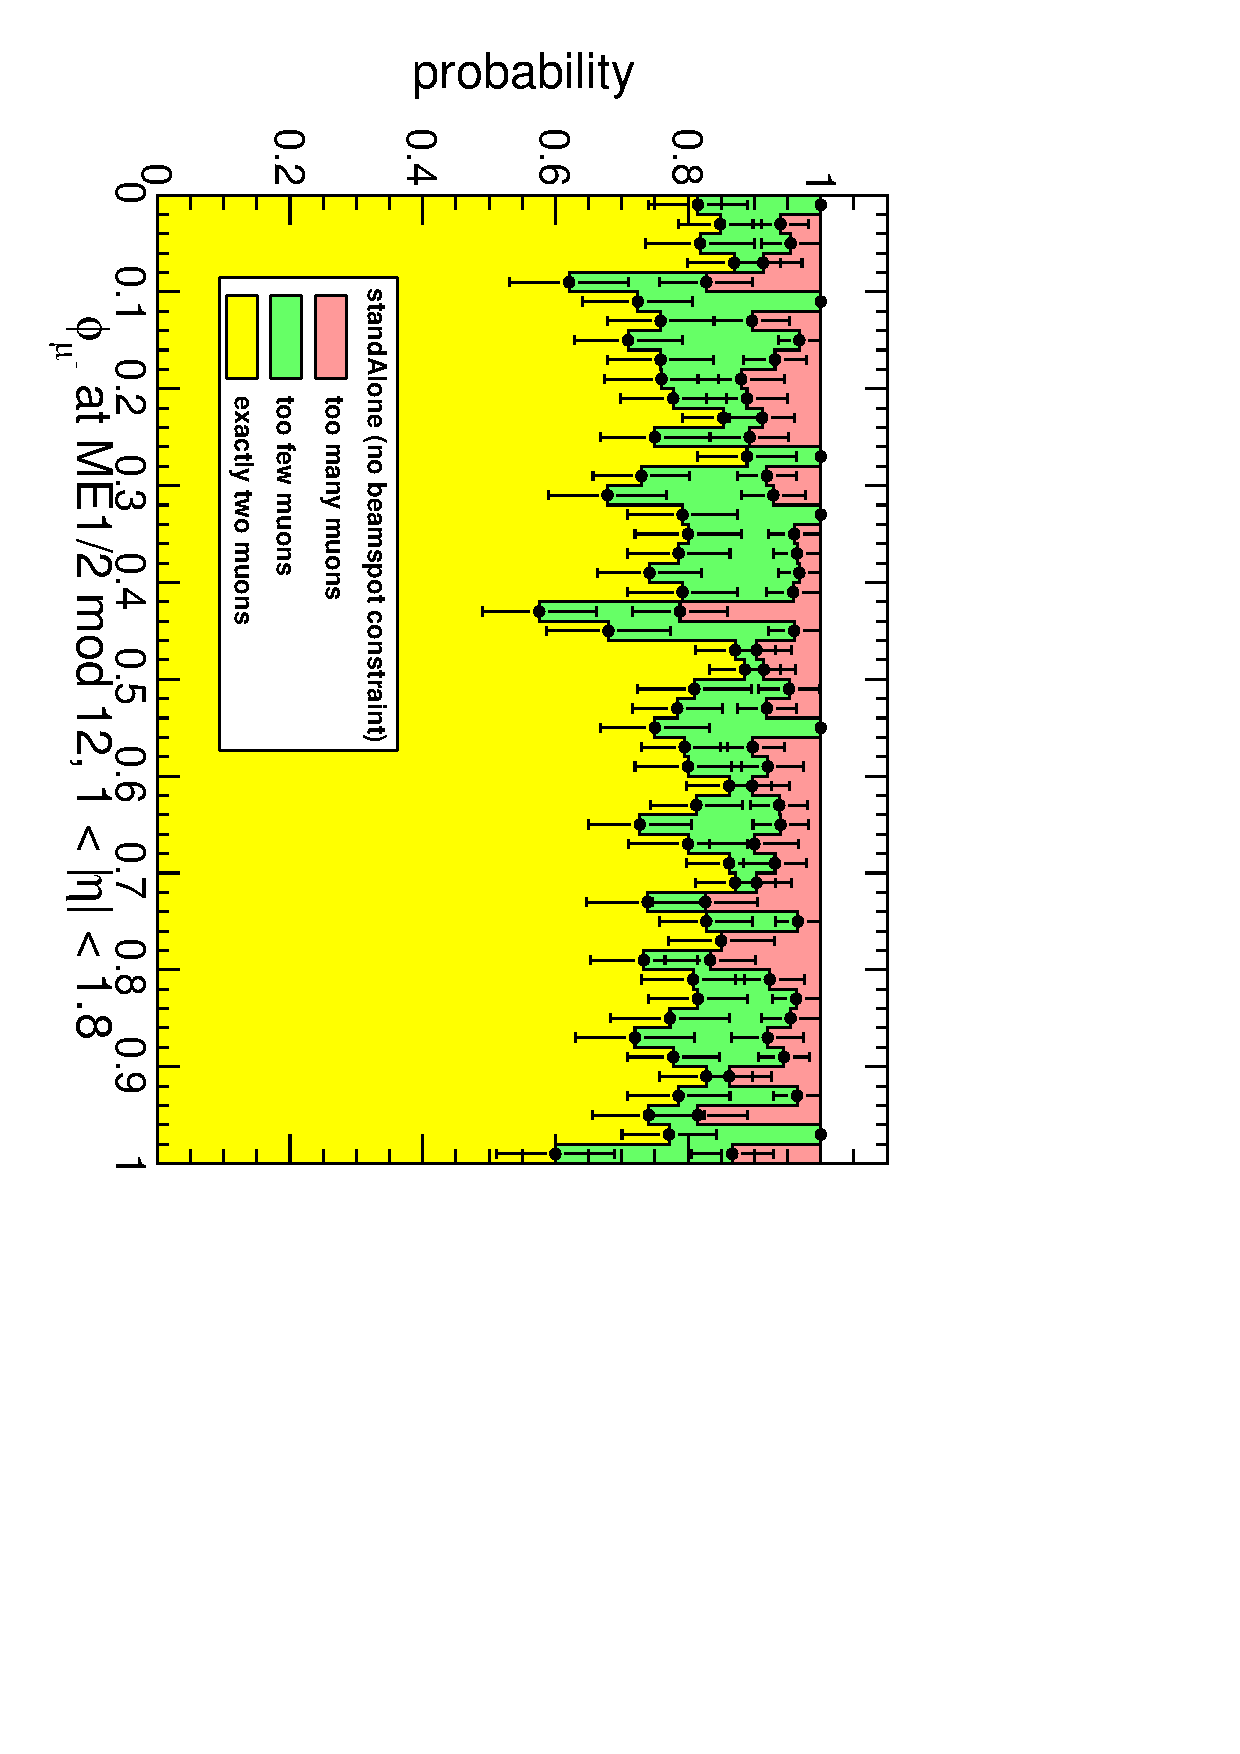
\includegraphics[height=0.33\linewidth, angle=90]{efficiency_standPhimod1.pdf}
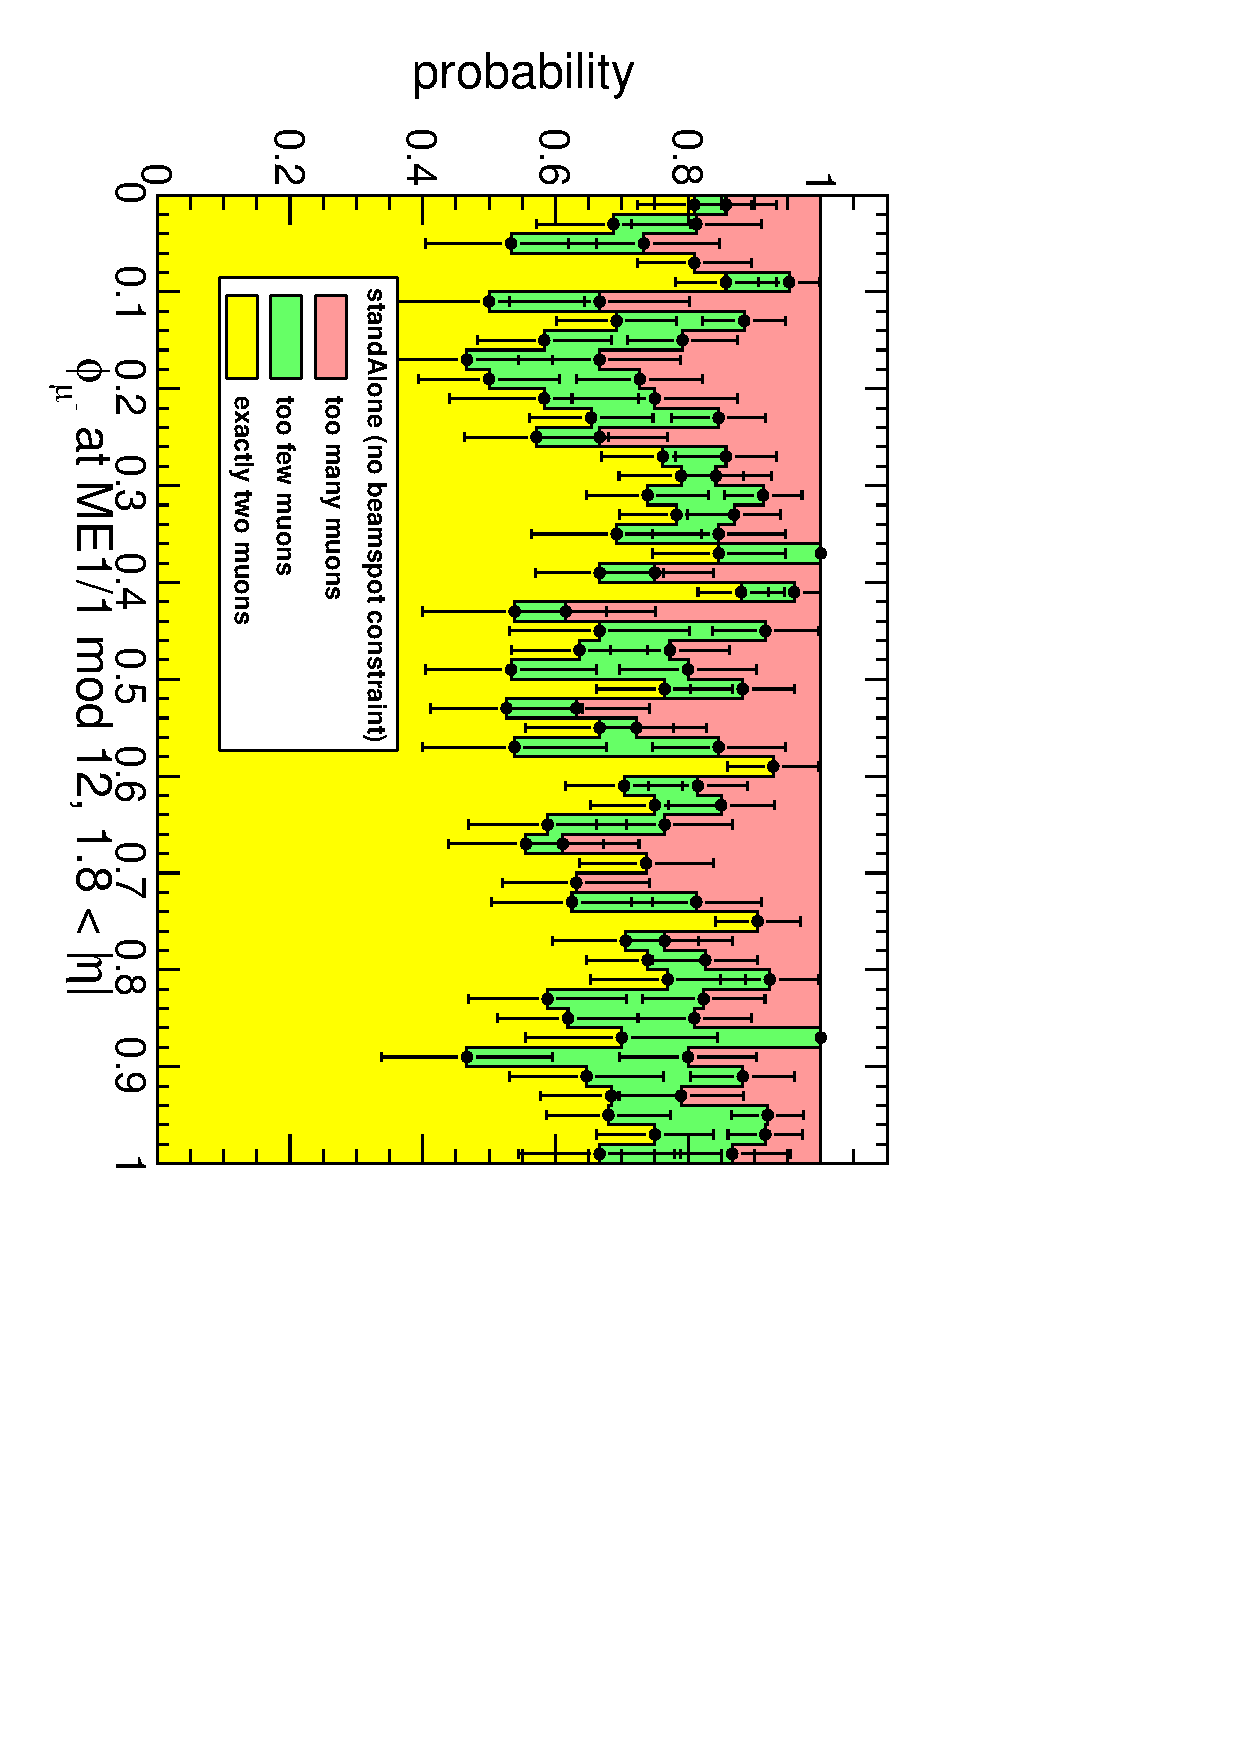
\includegraphics[height=0.33\linewidth, angle=90]{efficiency_standPhimod2.pdf}}
\end{frame}

\begin{frame}
\frametitle{Early misreconstruction studies}

\begin{columns}
\column{0.8\linewidth}
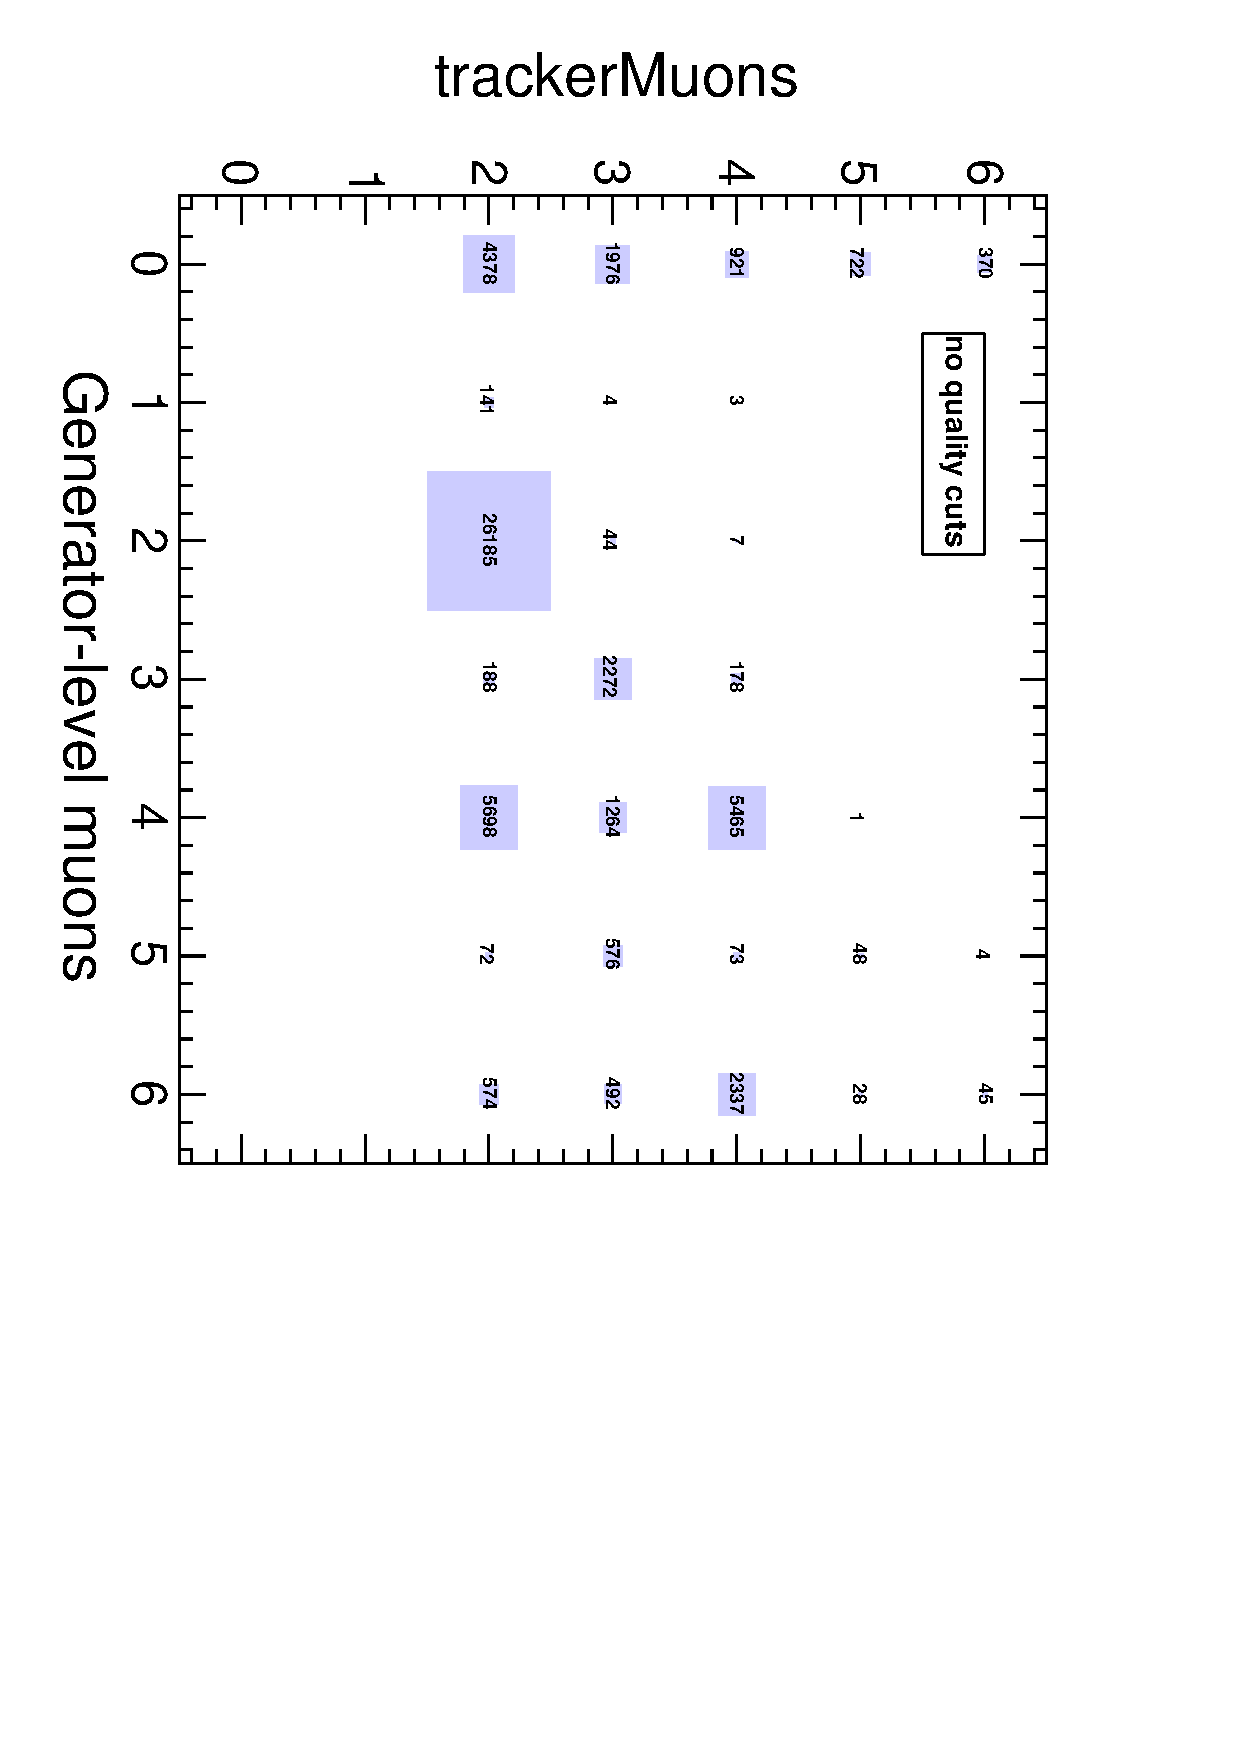
\includegraphics[height=0.5\linewidth, angle=90]{correlation_hgentracker.pdf}
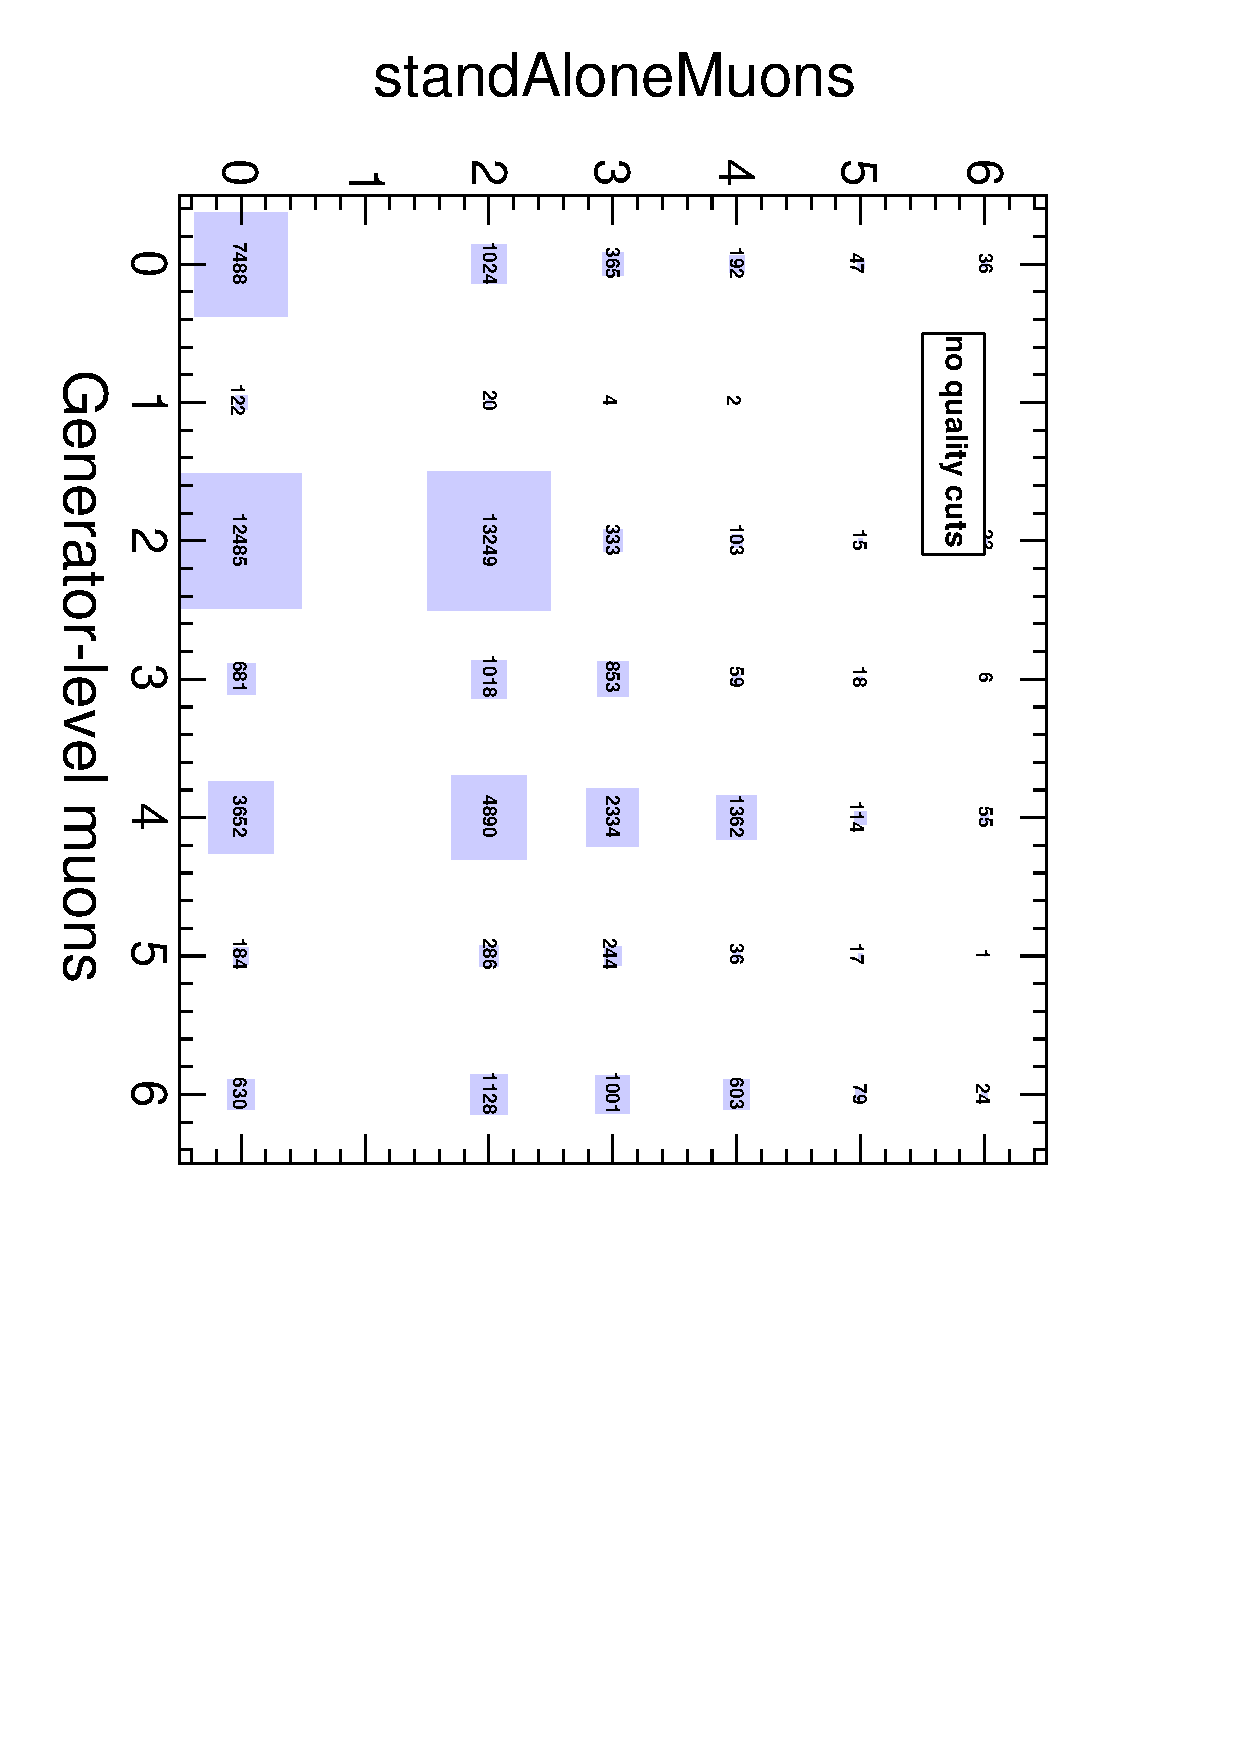
\includegraphics[height=0.5\linewidth, angle=90]{correlation_hgenstand.pdf}

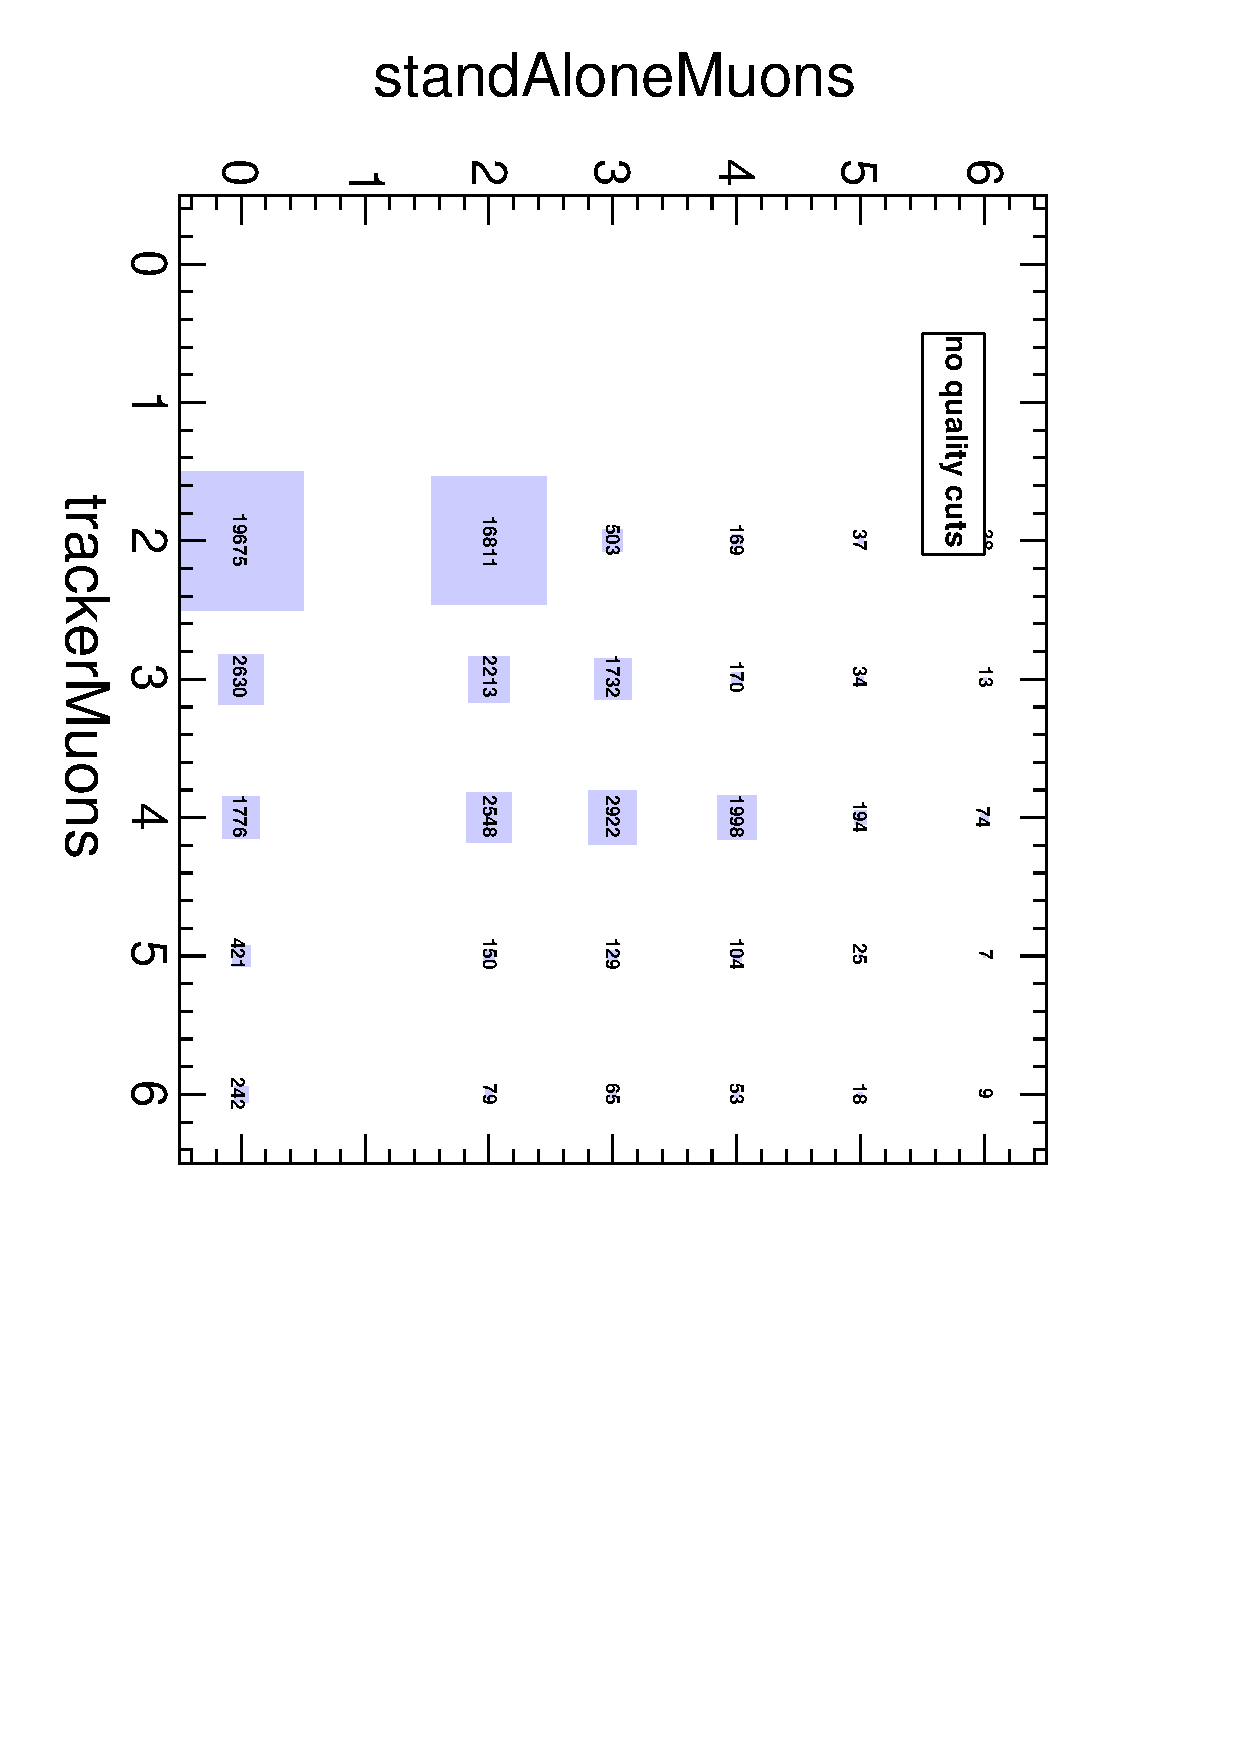
\includegraphics[height=0.5\linewidth, angle=90]{correlation_htrackerstand.pdf}
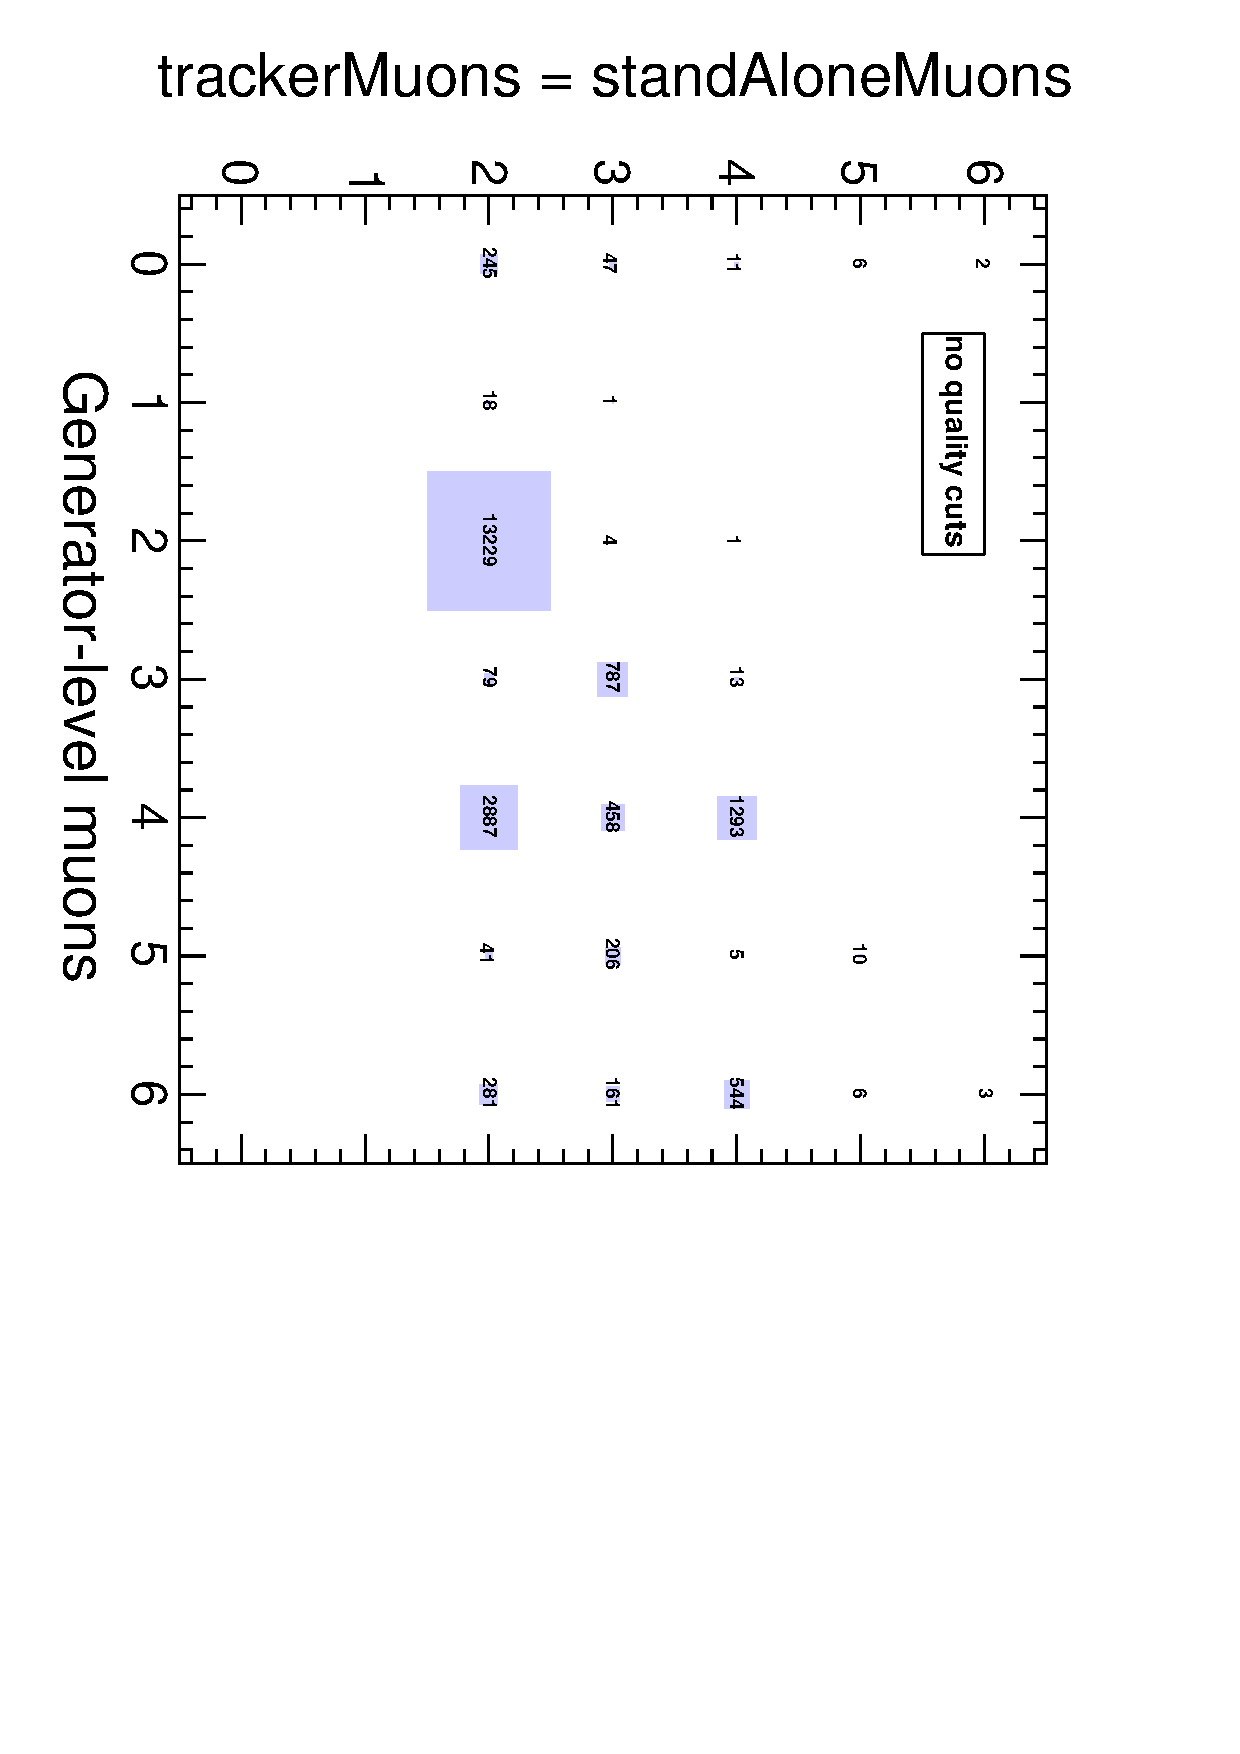
\includegraphics[height=0.5\linewidth, angle=90]{correlation_hgenagree.pdf}

\column{0.3\linewidth}
\begin{itemize}
\item Realistic model MC ($\mathcal{U}(1)_{\mbox{\scriptsize dark}}$) with underlying event and mul- tiple interactions

\item trackerMuons and standAloneMuons \mbox{independ-\hspace{-0.5 cm}} ently grouped;
  comparing $N_{\mbox{\scriptsize muons per group}}$ {\scriptsize (with $|\eta| < 2.4$ and $p_T > 2.5$~GeV)}

\item We can see trackerMuon fakes and stand- AloneMuon inefficiencies
\end{itemize}
\end{columns}
\end{frame}

\begin{frame}
\frametitle{Mass/momentum resolution}

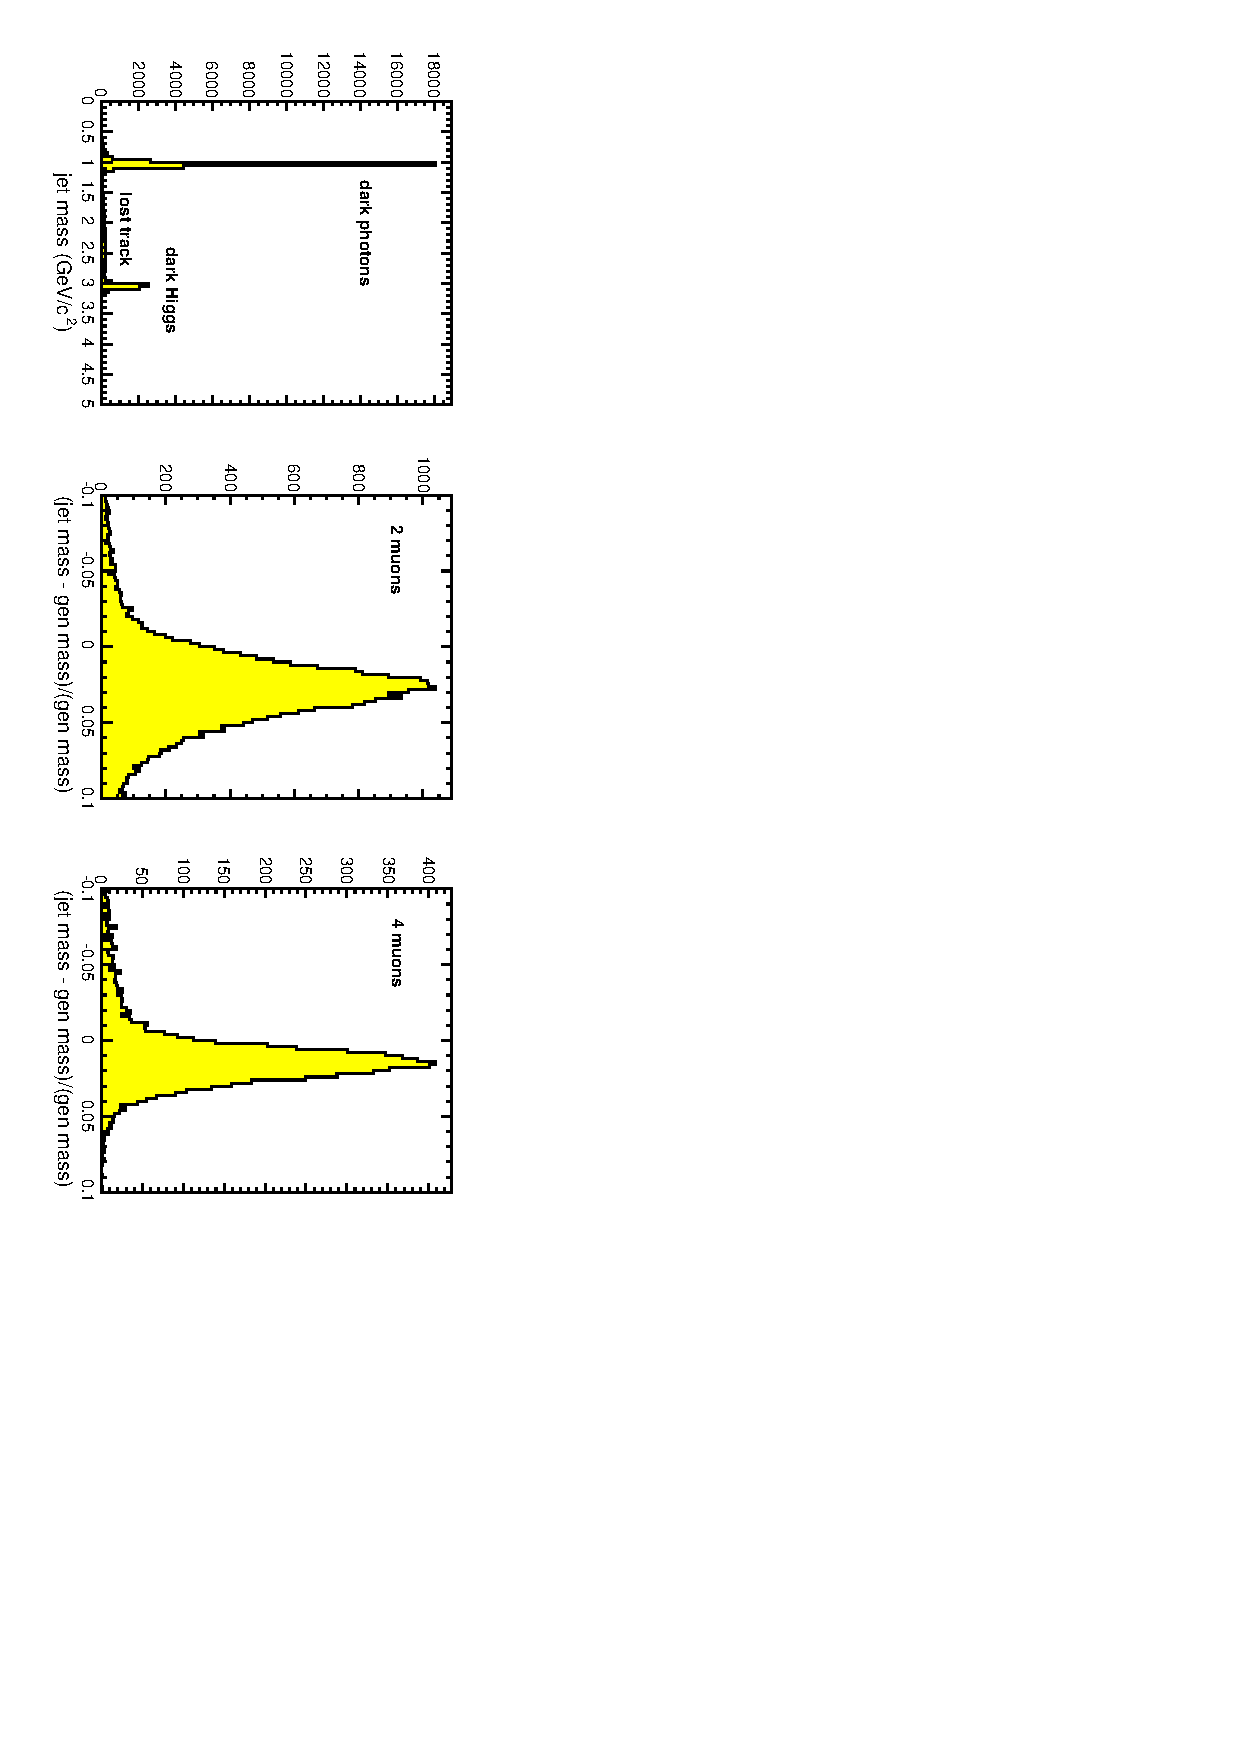
\includegraphics[height=\linewidth, angle=90]{spectra_mass.pdf}

\hfill 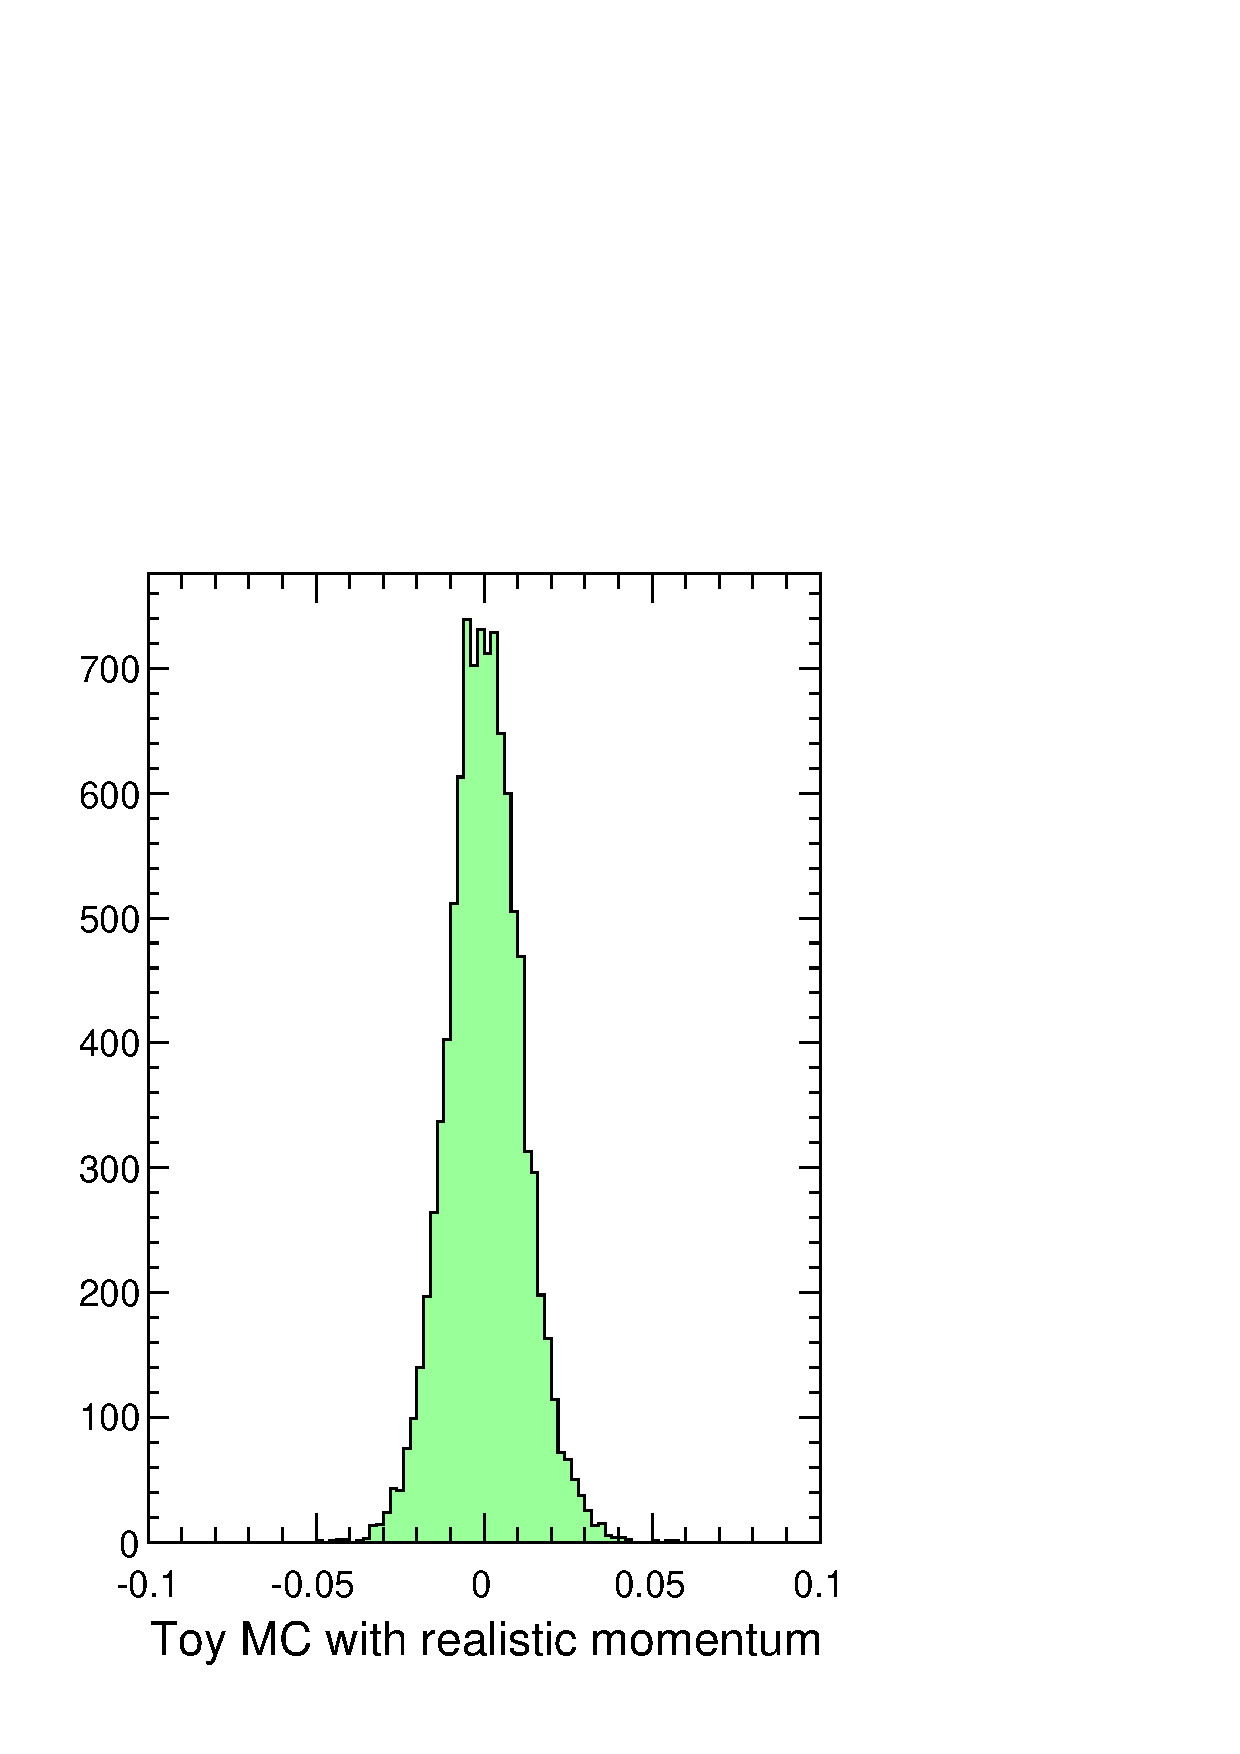
\includegraphics[height=4 cm]{toymc_mass_resolution.pdf} 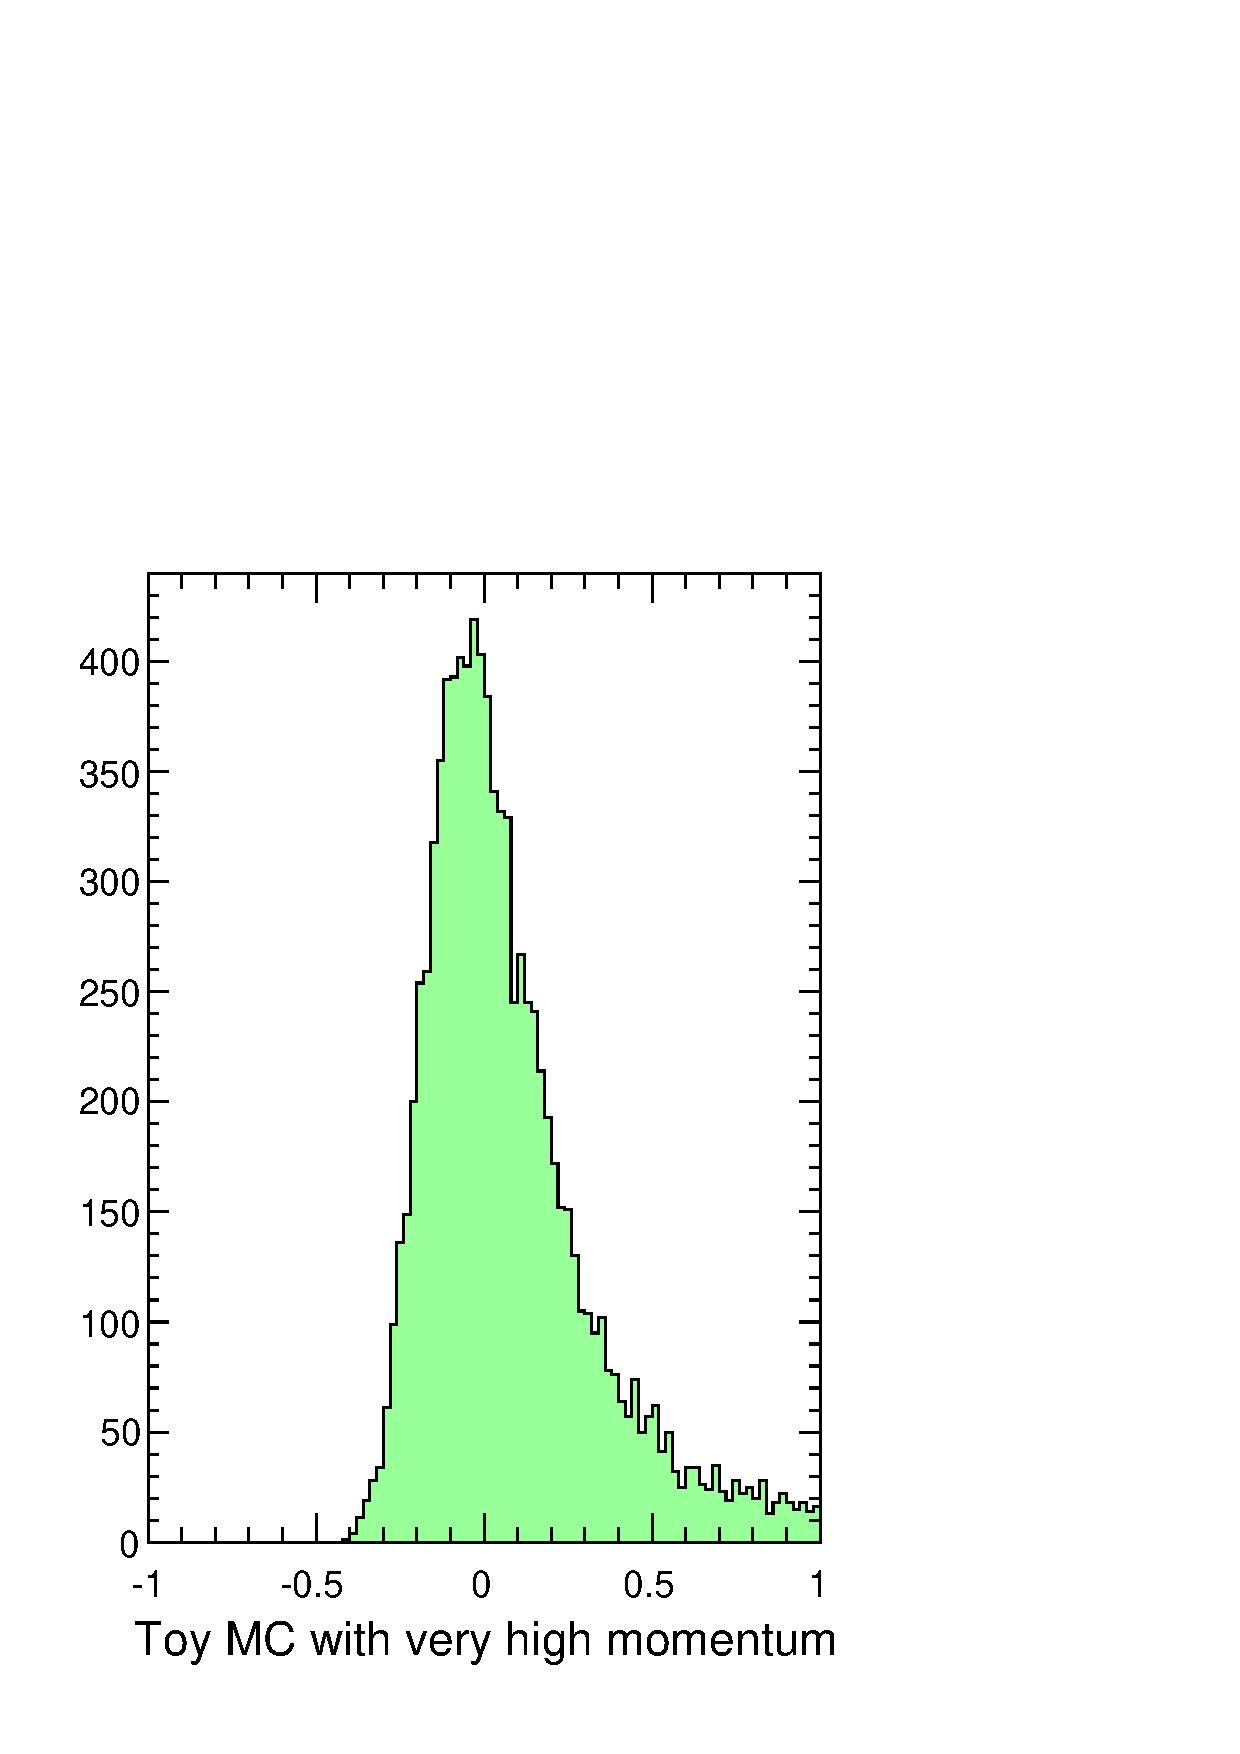
\includegraphics[height=4 cm]{toymc_mass_resolution2.pdf}

\vspace{-4 cm}
\begin{itemize}
\item $\mathcal{O}($1--3\%$)$ bias in mass of \\ trackerMuon jets
\item Boosted mass distributions \\ can be asymmetric because \\ $\Delta
  p_T$ is one-sided, but that's \\ not responsible for the above \\
  asymmetry
\end{itemize}
\end{frame}

\begin{frame}
\frametitle{Software framework}

\begin{itemize}
\item pat::MultiMuonCandidate represents a group of nearby muons
\begin{itemize}
\item useful for organizing muon jet analyses:

\vspace{0.1 cm}
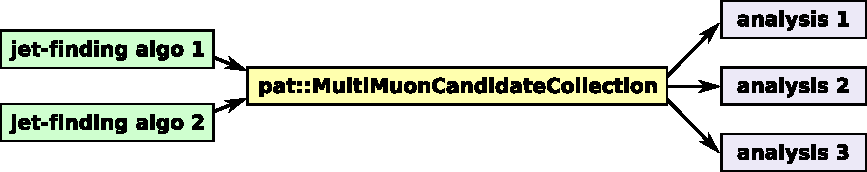
\includegraphics[width=0.9\linewidth]{jets_to_analyses.pdf}

\end{itemize}

\item Provides useful variables for cuts, pre-calculated:
\begin{itemize}
\item vertexing, vertex probability
\item isolation (properly ignoring the muons in the isolation cone)
\item matching trackerMuonJets and standAloneMuonJets for comparison
\item variables to identify ME1/1a triplets
\item propagating MC match to composite object
\end{itemize}

\item Simple clustering algorithm LeptonJetsEquivalenceClassProducer
\begin{itemize}
\item all muons within a given $\Delta R$ of a group are included in the group
\end{itemize}
\end{itemize}
\end{frame}

\begin{frame}
\frametitle{Software framework}

\vfill
Example event display, illustrating pat::MultiMuonCandidate variables

\vfill
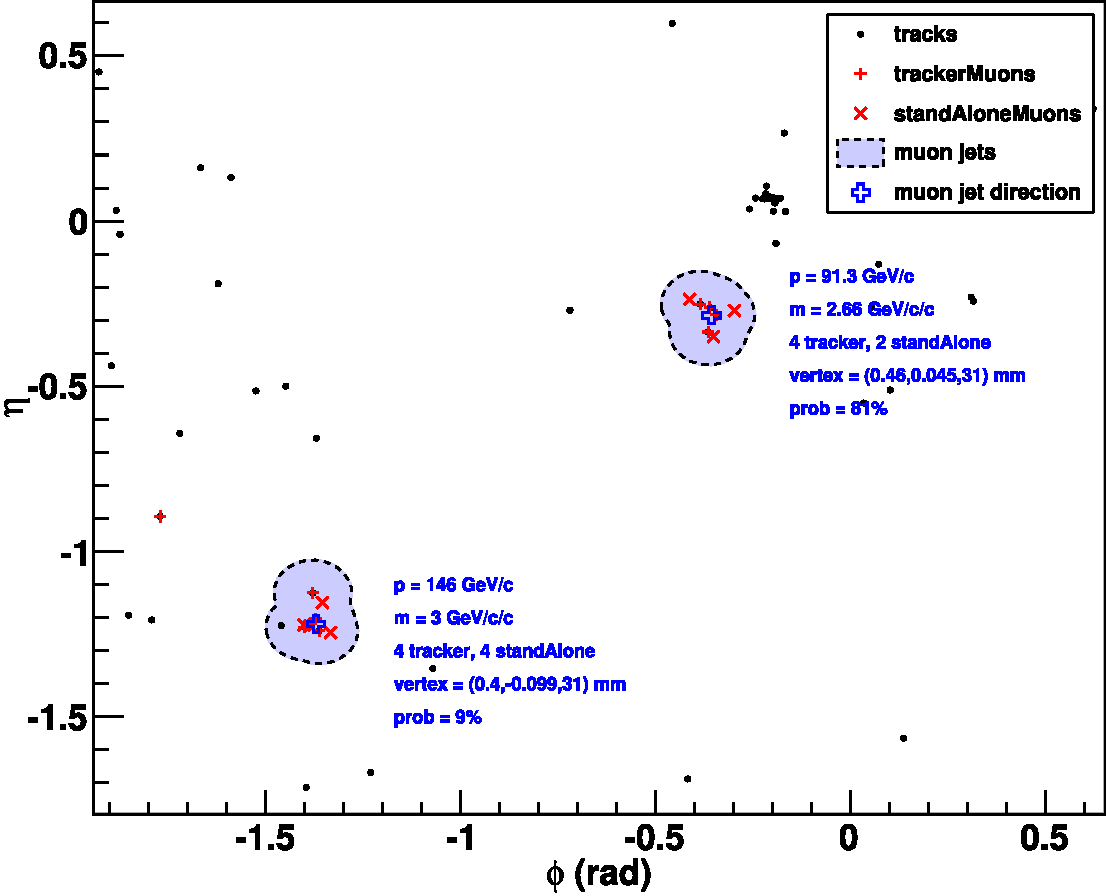
\includegraphics[width=0.85\linewidth]{example_event_display_3.pdf}
\end{frame}

\begin{frame}
\frametitle{Software framework}

\begin{columns}
\column{0.7\linewidth}
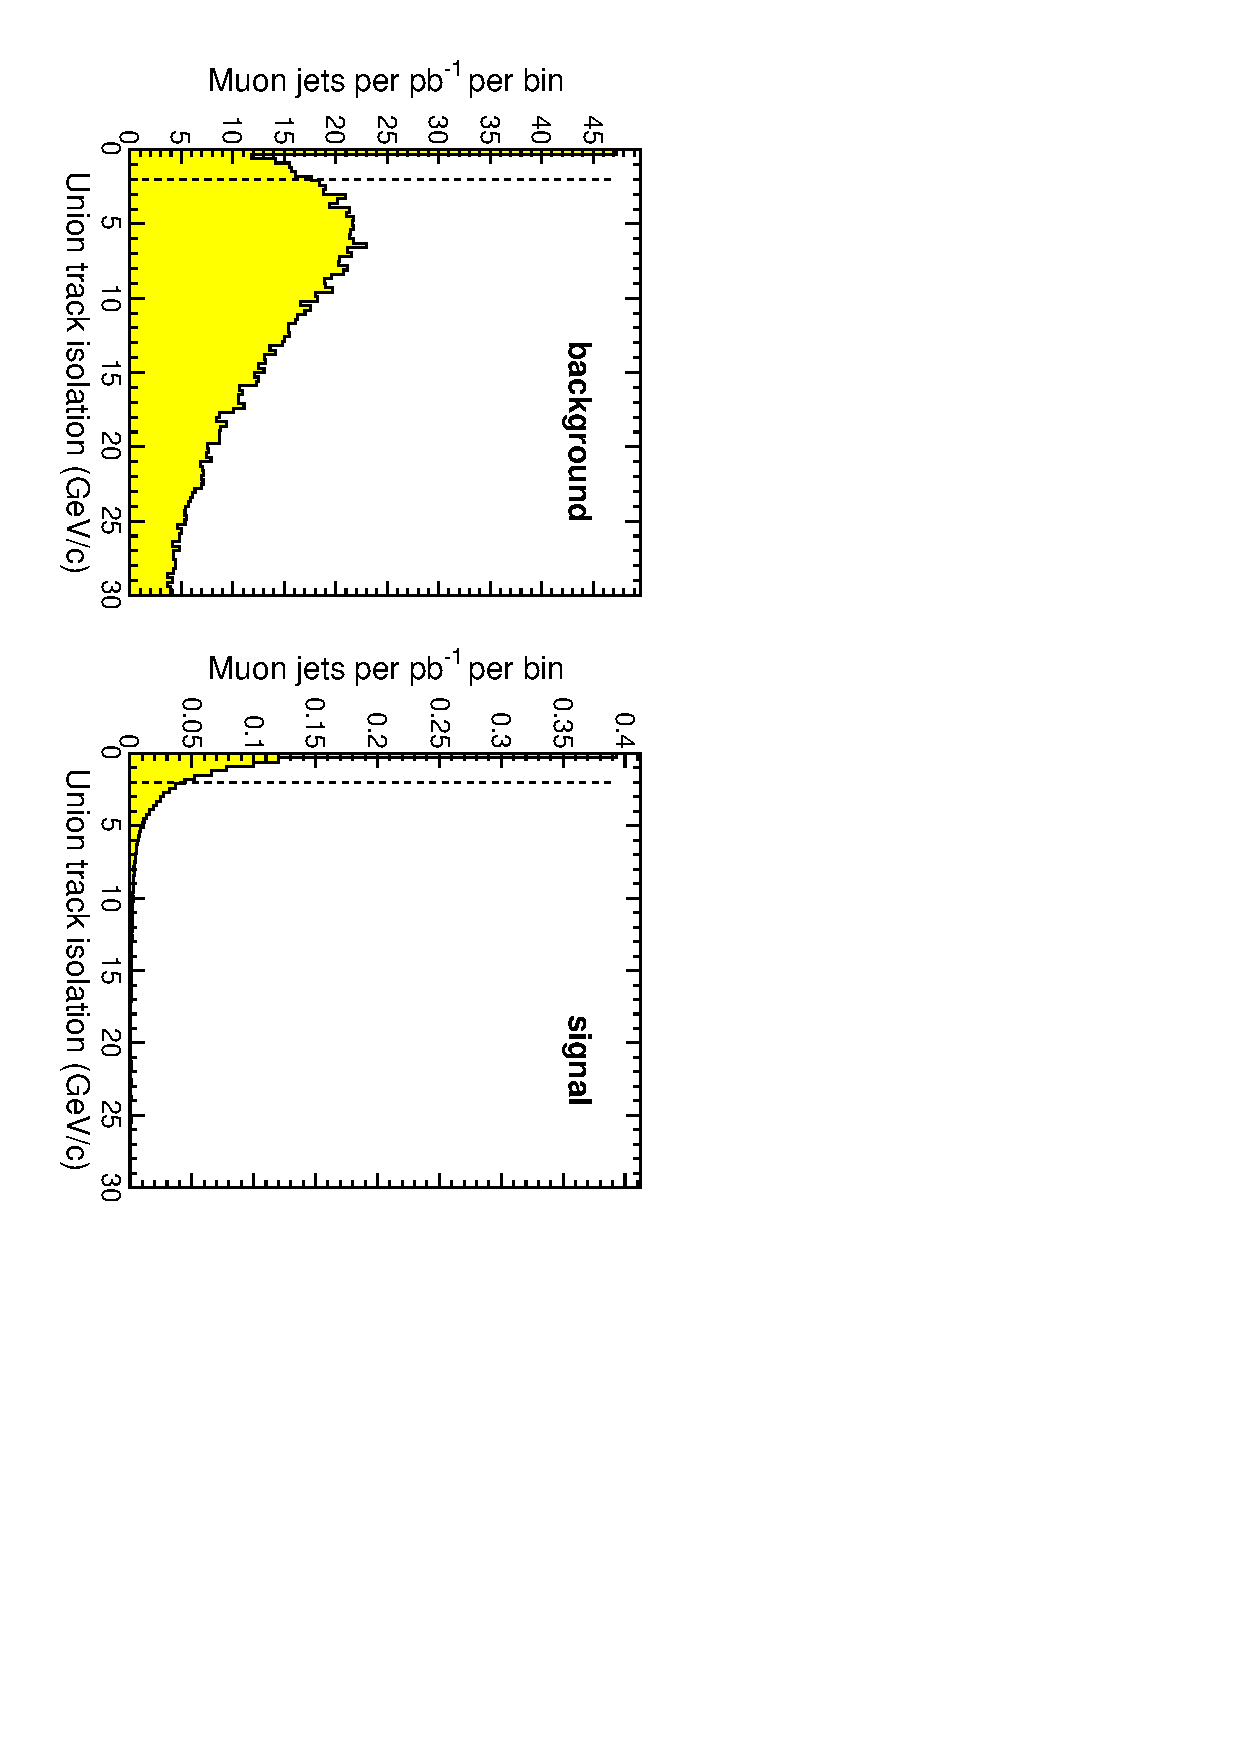
\includegraphics[height=\linewidth, angle=90]{backgrounds_isolation_muontrack.pdf}

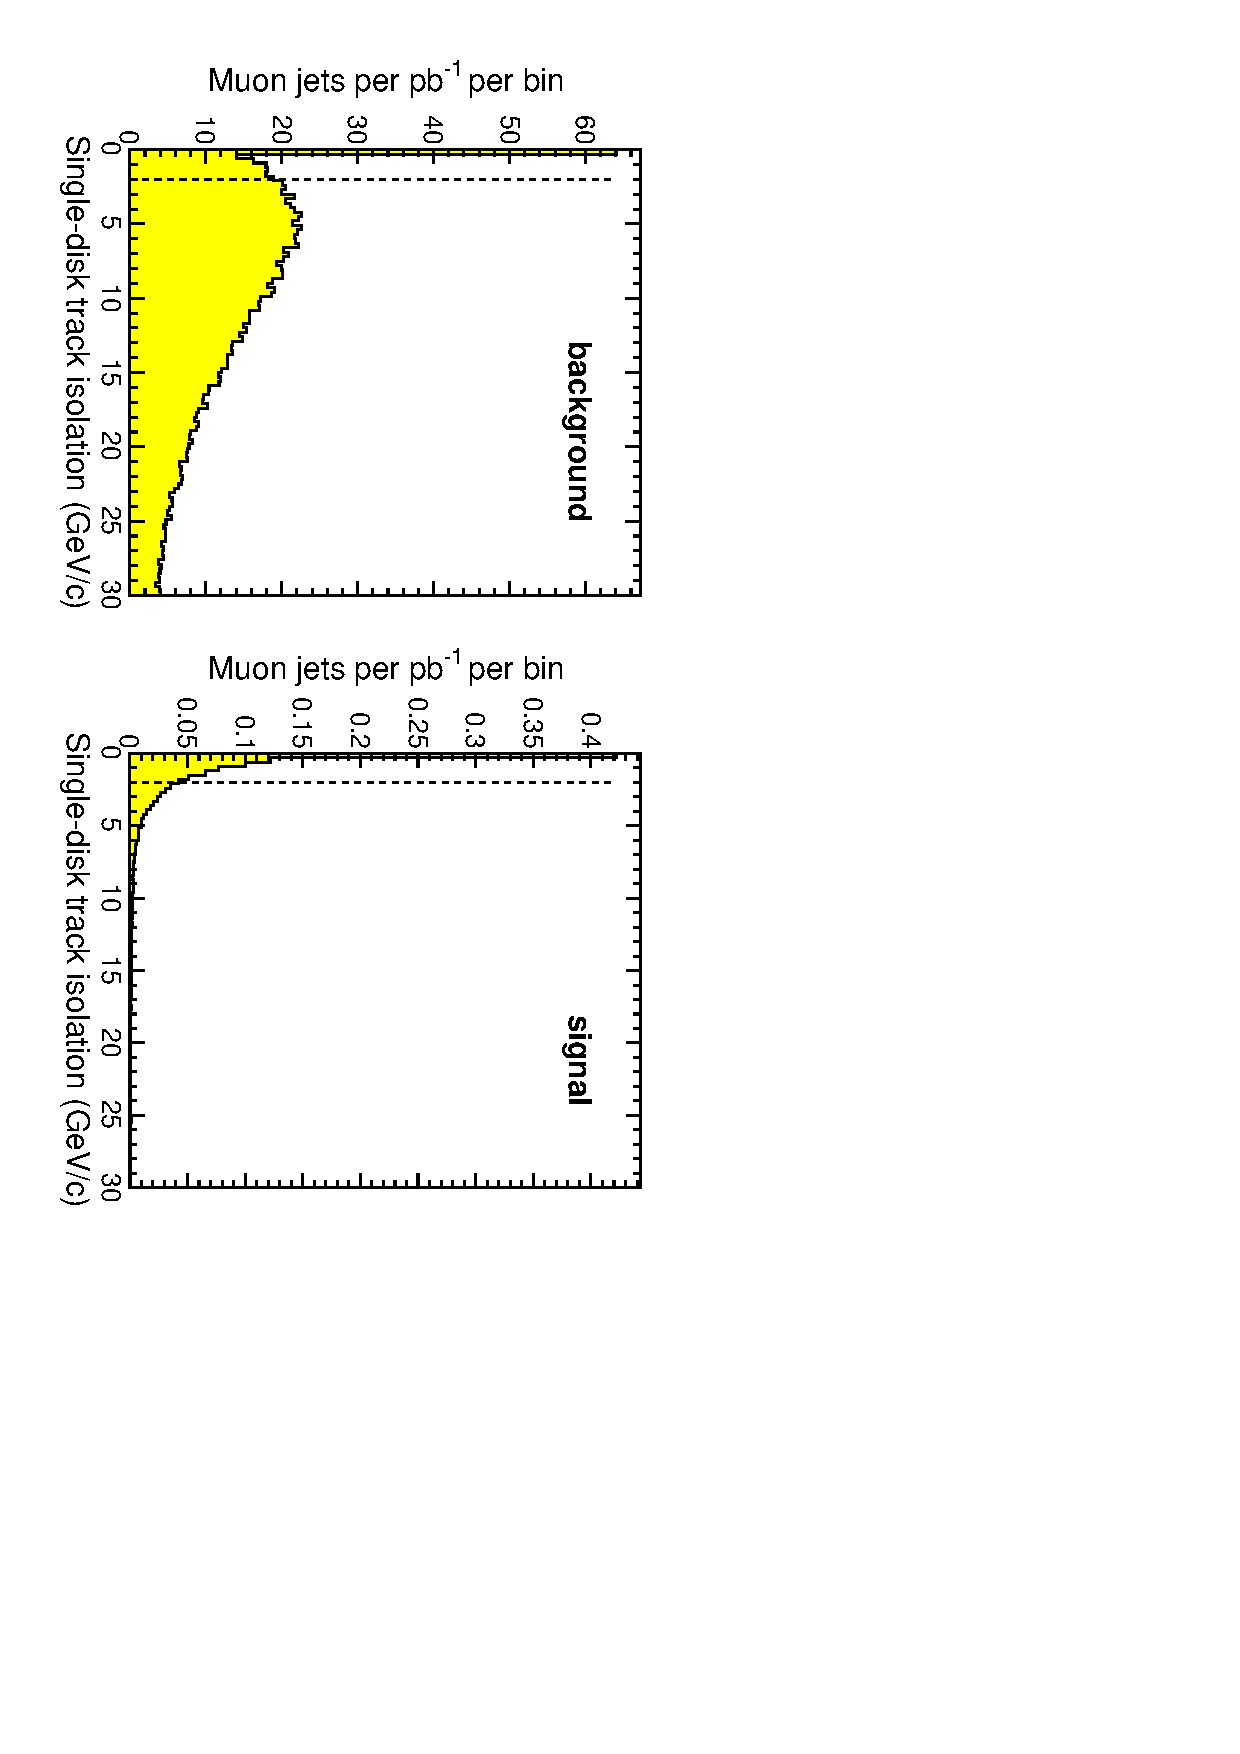
\includegraphics[height=\linewidth, angle=90]{backgrounds_isolation_jpsitrack.pdf}

\column{0.4\linewidth}

\begin{itemize}
\item $\sum p_T$ in isolation cone must not count the other muons in
  the cone, and must not double-count overlapping cones

\item Multi-muon cone definitions:

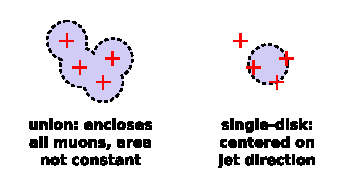
\includegraphics[width=\linewidth]{isolation_variables.pdf}

\item Single-disk is preferred because the area is constant
  (backgrounds are uniform in $\eta$-$\phi$)
\end{itemize}
\end{columns}
\end{frame}

\begin{frame}
\frametitle{Software framework}

\begin{columns}
\column{0.7\linewidth}

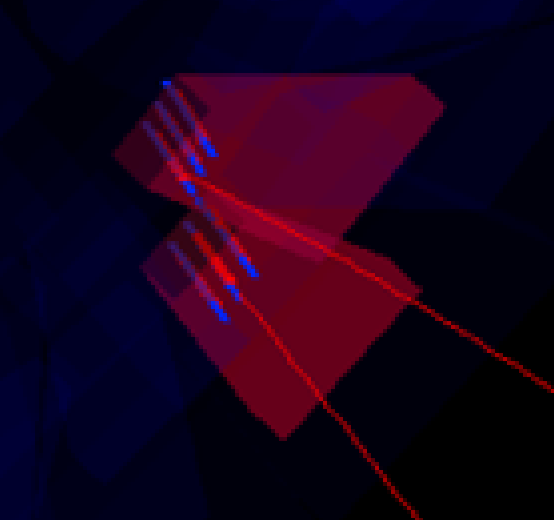
\includegraphics[width=0.45\linewidth]{triplet_closeup.png}
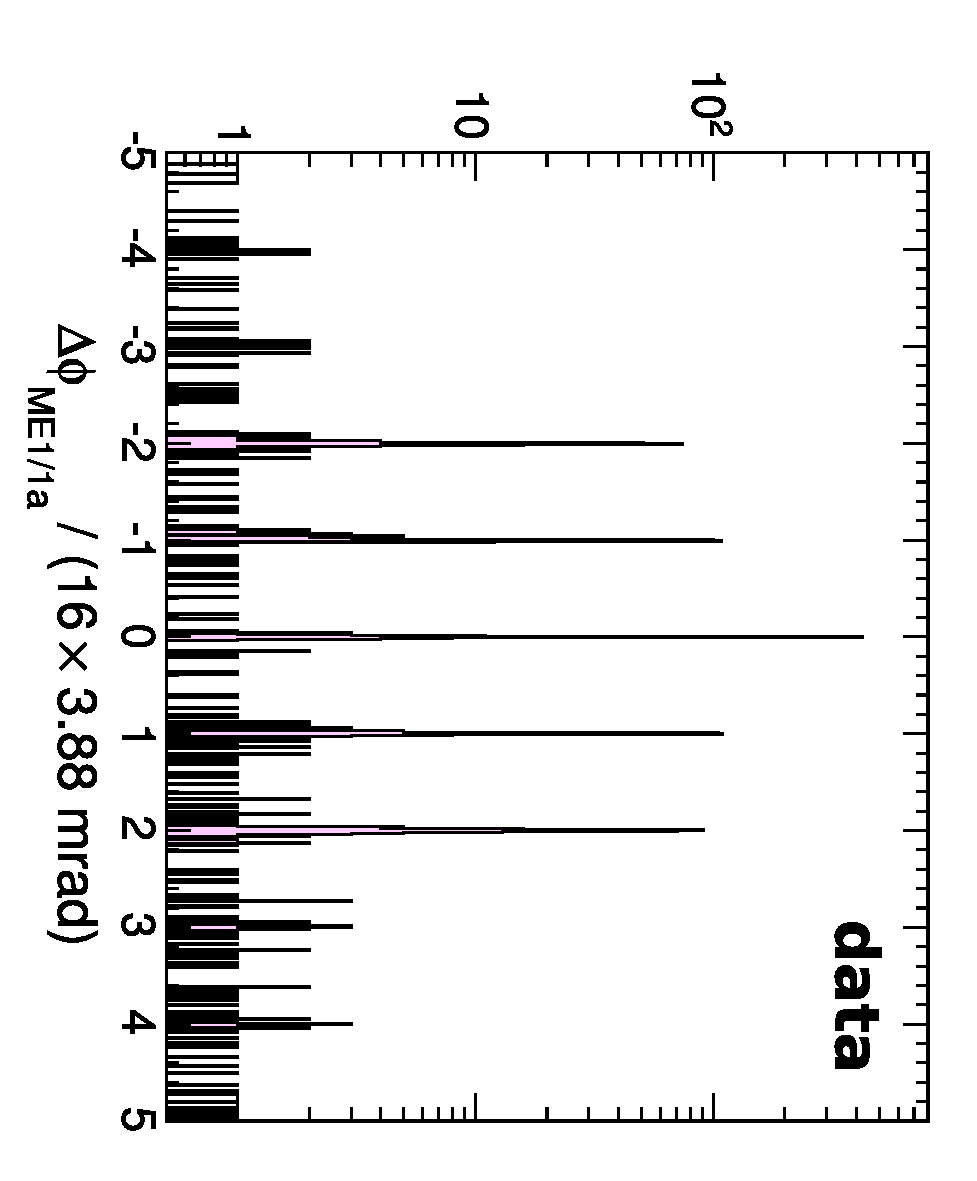
\includegraphics[height=0.55\linewidth, angle=90]{gangedstripcut.pdf}

\vspace{0.3 cm}
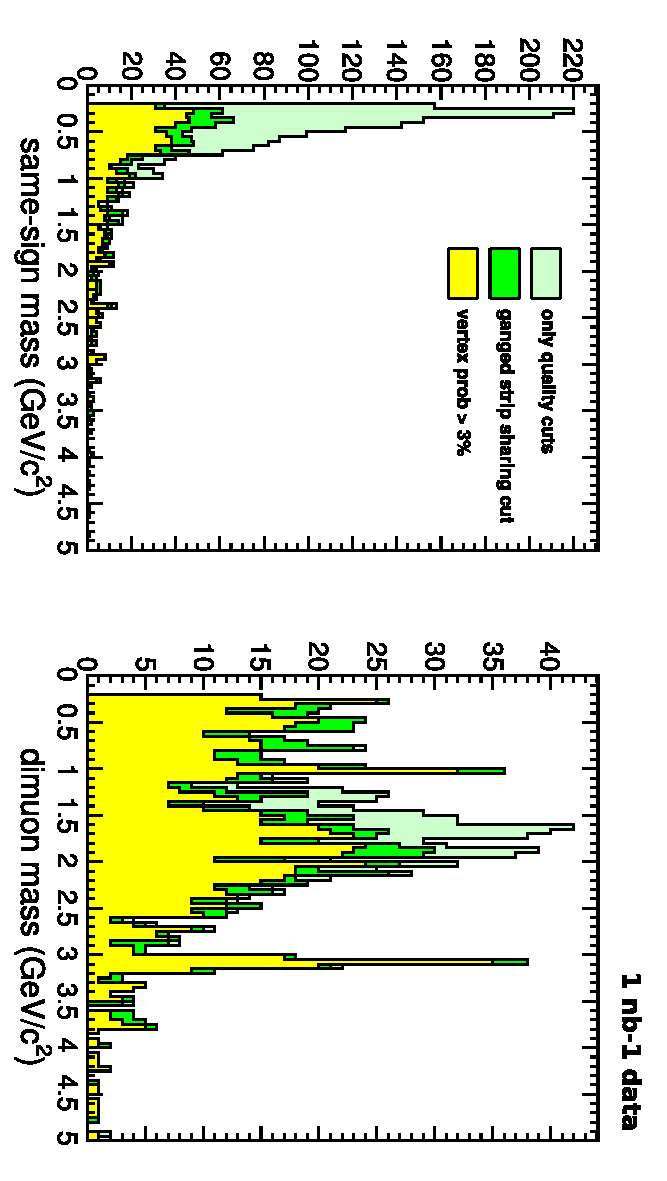
\includegraphics[height=\linewidth, angle=90]{gangedstripcut_mass.pdf}

\column{0.35\linewidth}
\begin{itemize}
\item ME1/1a strips are ganged, generating fake segments and therefore
  fake muon pairs (and triplets) in the forward region

\item Variables included to identify such cases

\item Bottom: cleaning real data without losing $J/\psi$ or
  $\phi(1020)$ peaks
\end{itemize}
\end{columns}
\end{frame}

%% \section*{First section}
%% \begin{frame}
%% \begin{center}
%% \Huge \textcolor{blue}{First section}
%% \end{center}
%% \end{frame}

\begin{frame}
\frametitle{Conclusions}

\begin{itemize}\setlength{\itemsep}{0.5 cm}
\item There are several ways that lepton jets can distinguish themselves from background; target searches for each general case

\item Aysen's (A\&M) physics interests are in case \textcolor{blue}{(b)}

\item We'll need to consider misreconstruction as both an inefficiency and as a major background

\item We've developed a software framework for organizing these studies
\end{itemize}

\label{numpages}
\end{frame}

\begin{frame}
\begin{center}
\textcolor{blue}{\Large BACKUP}
\end{center}
\end{frame}

\begin{frame}
\frametitle{$|\vec{p}|$, $m$ vs.\ opening angle}
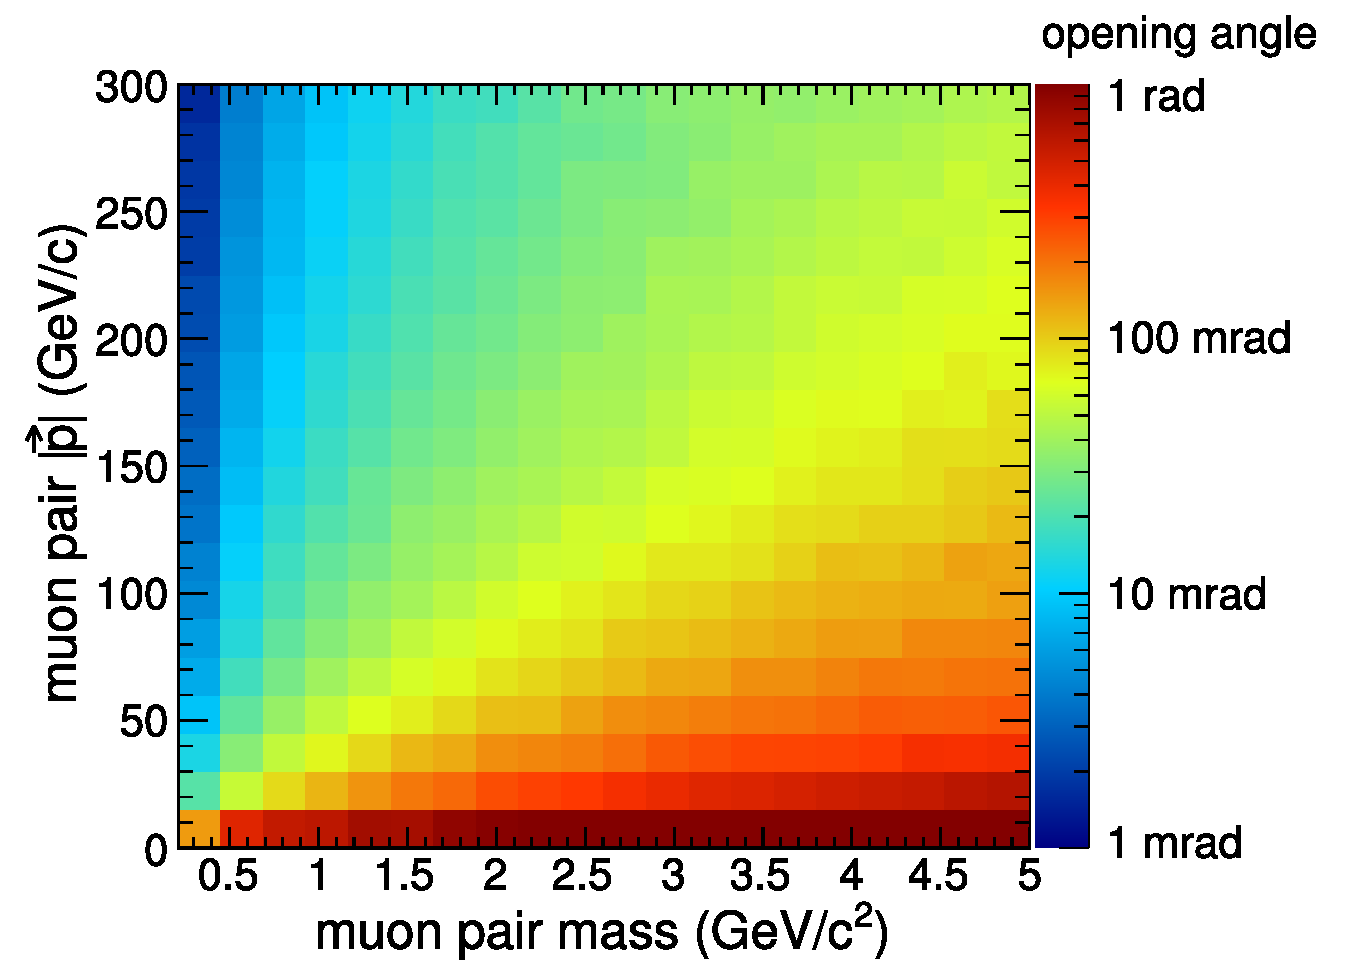
\includegraphics[width=\linewidth]{openingangle_angle.pdf}
\end{frame}

\begin{frame}
\frametitle{$p_T$, $m$ vs.\ track separation}

\only<1>{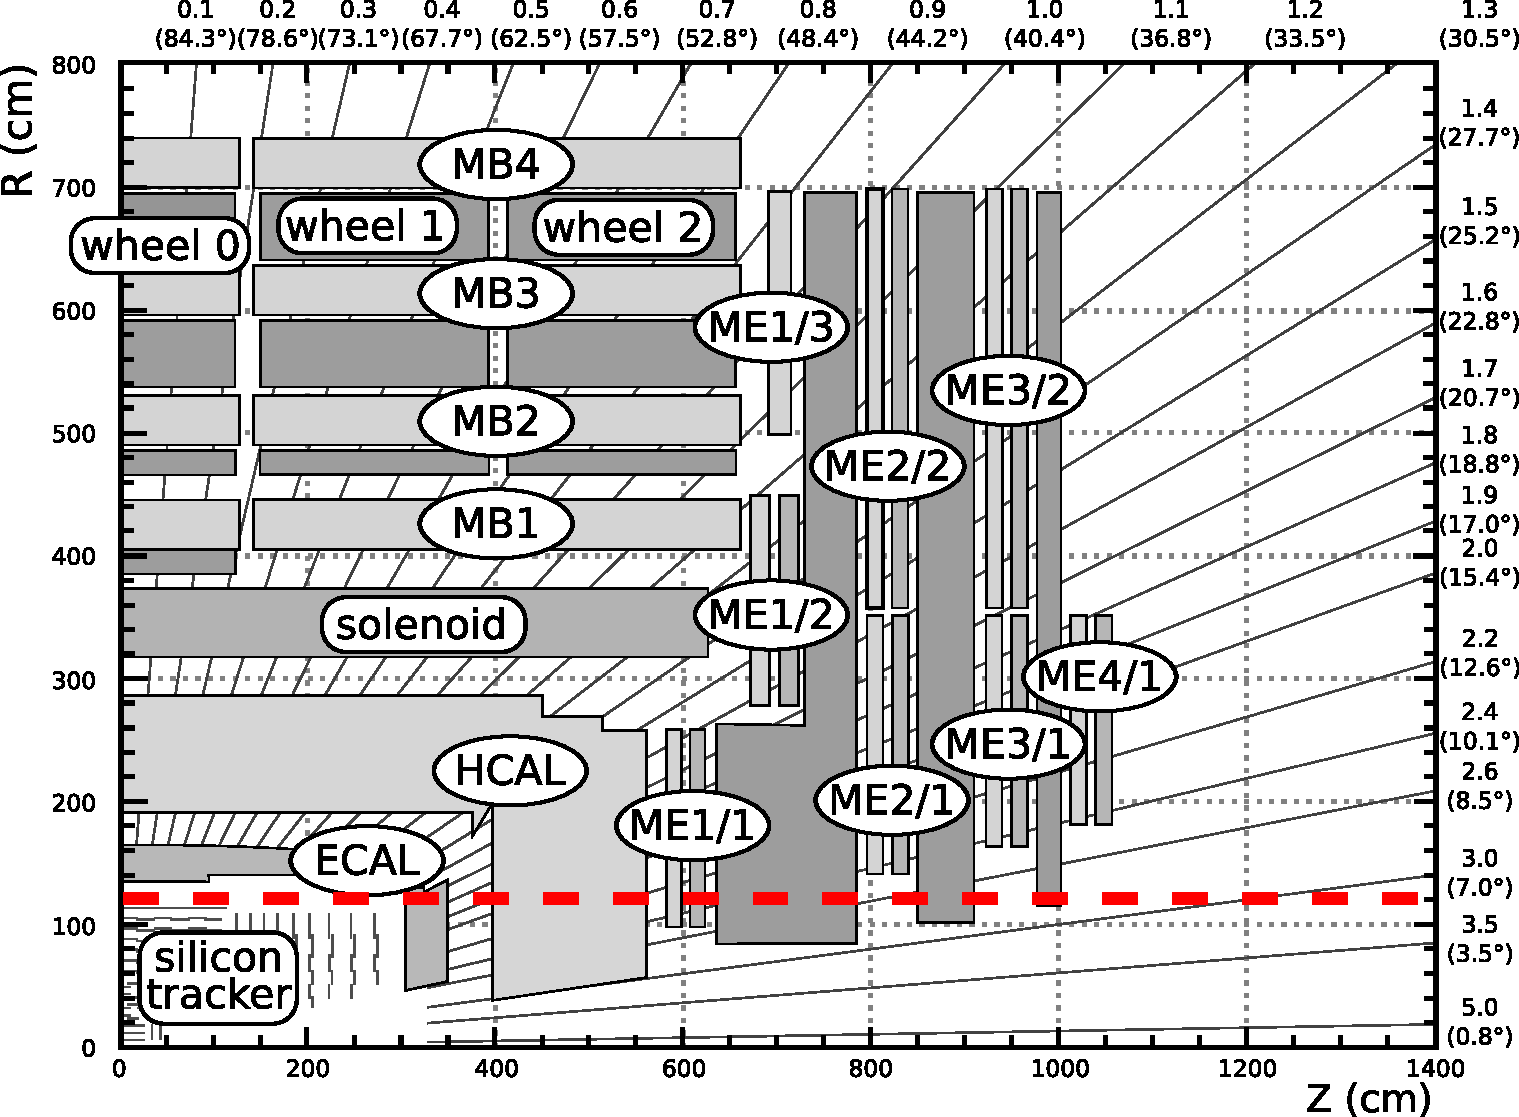
\includegraphics[width=0.4\linewidth]{muon_system_labeled2_outerTrackerMax.pdf} \\ 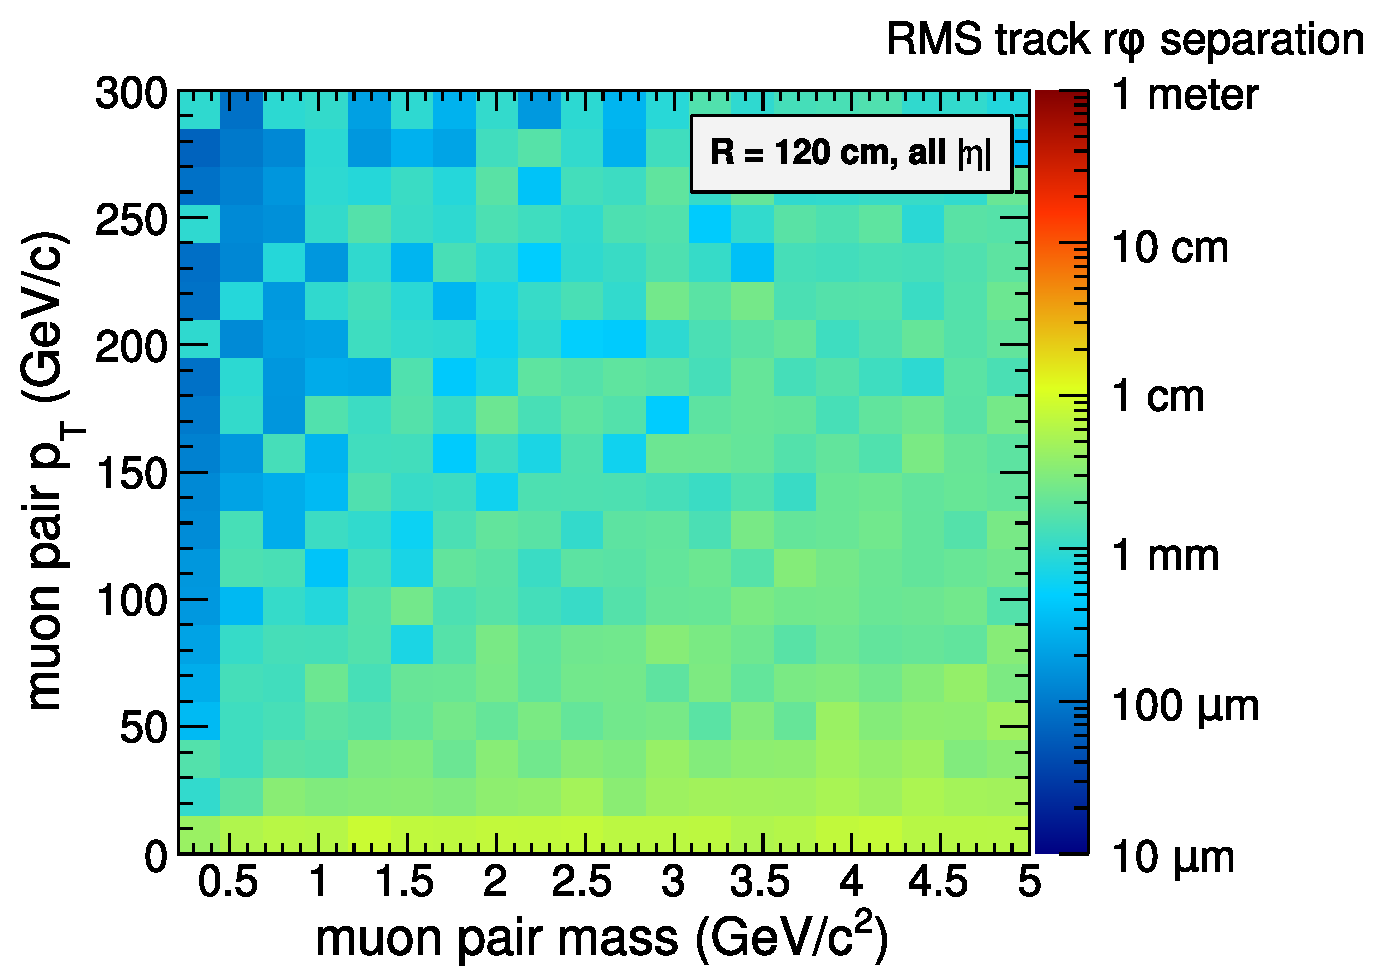
\includegraphics[width=0.7\linewidth]{openingangle_outerTrackerMax.pdf}}
\only<2>{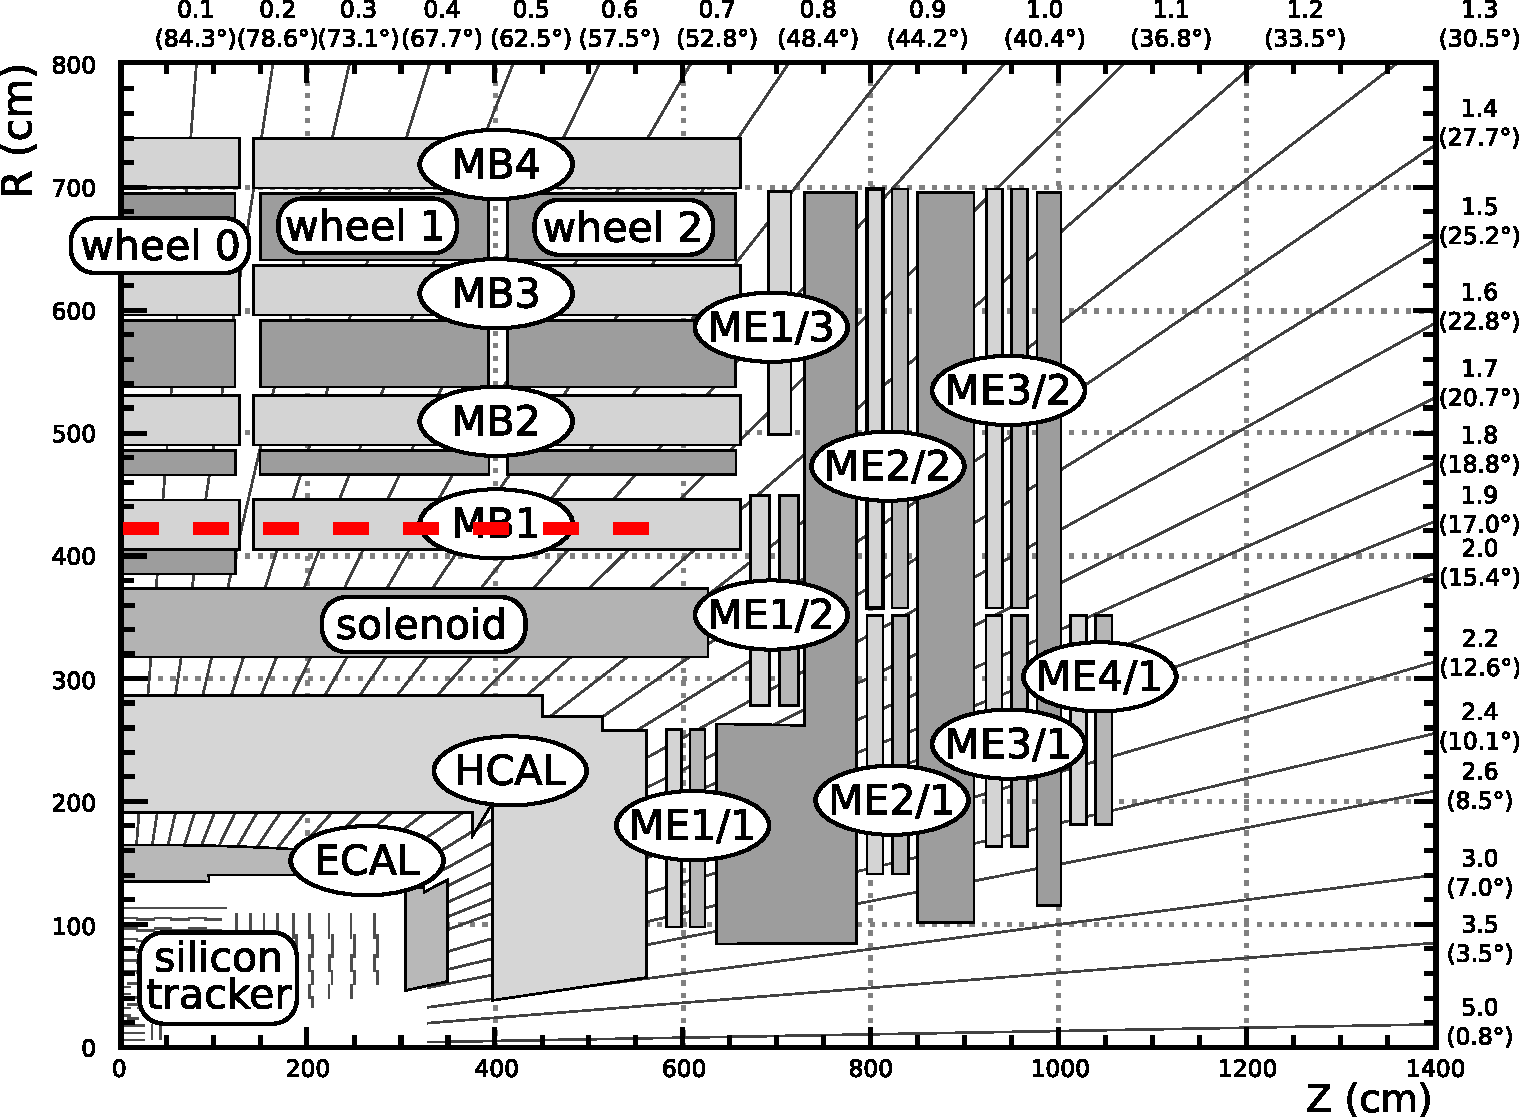
\includegraphics[width=0.4\linewidth]{muon_system_labeled2_station1Max.pdf} \\ 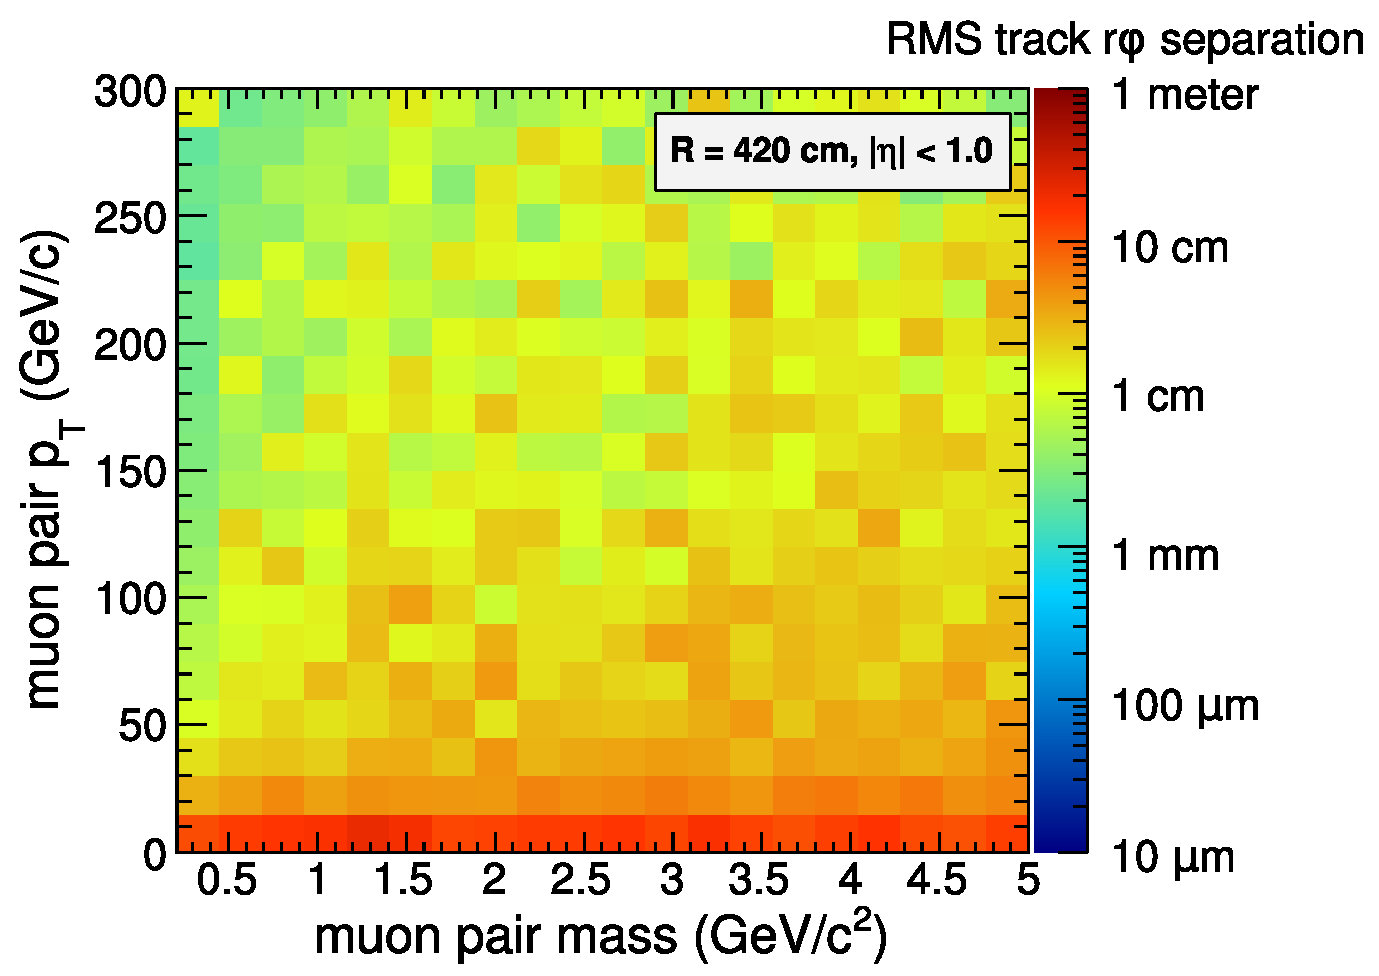
\includegraphics[width=0.7\linewidth]{openingangle_station1Max.pdf}}
\only<3>{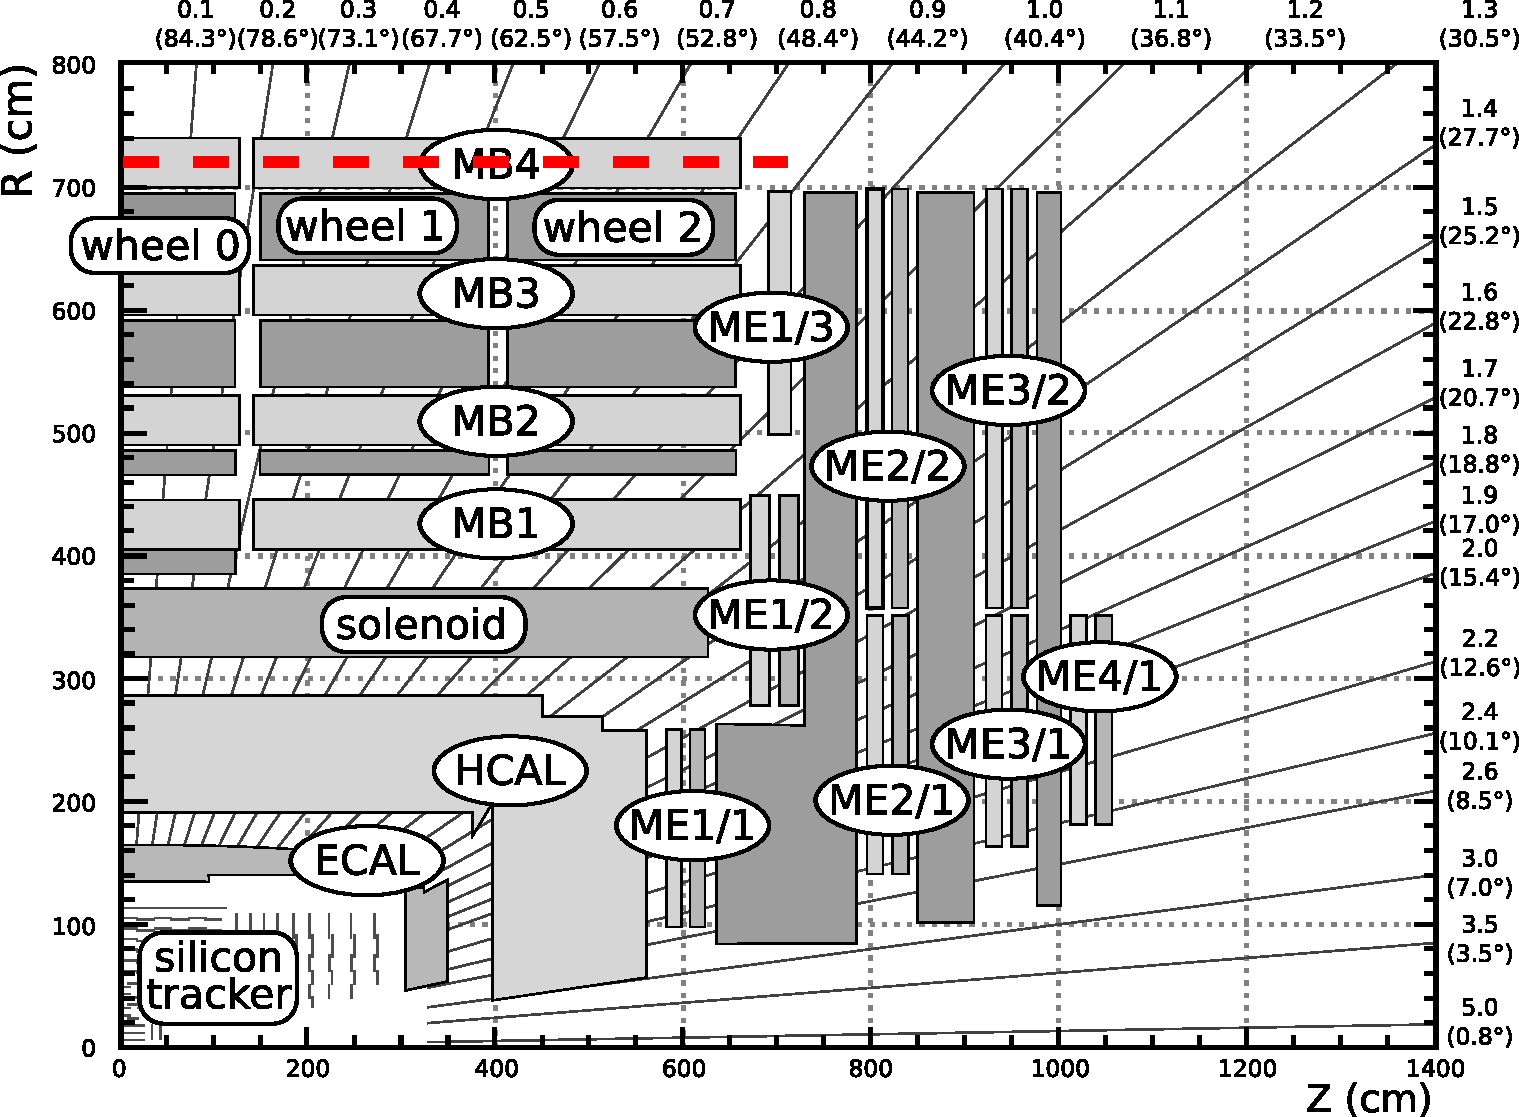
\includegraphics[width=0.4\linewidth]{muon_system_labeled2_station4Max.pdf} \\ 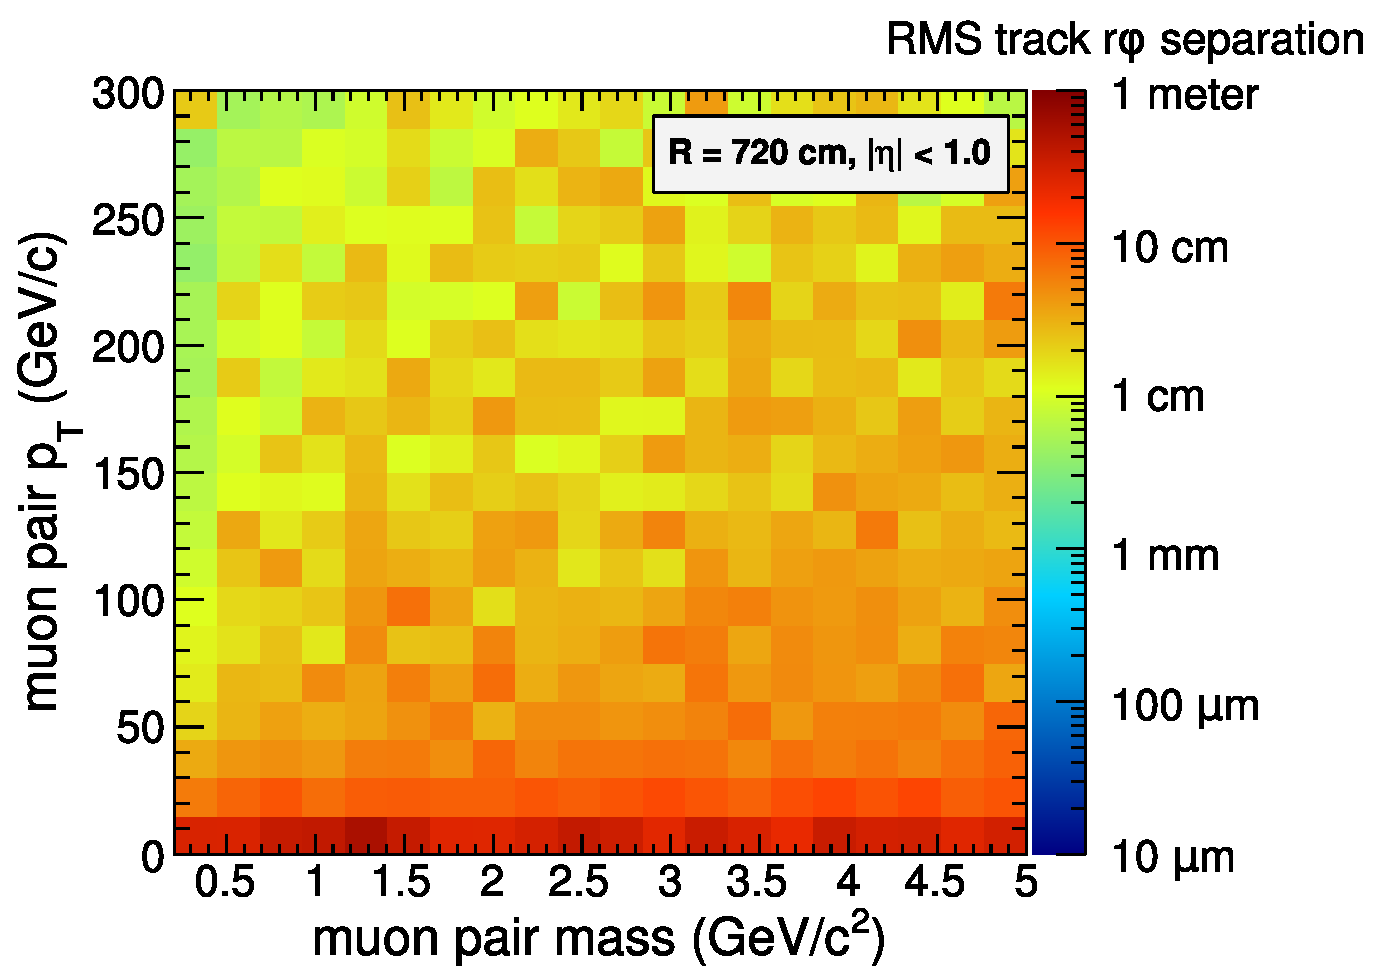
\includegraphics[width=0.7\linewidth]{openingangle_station4Max.pdf}}
\only<4>{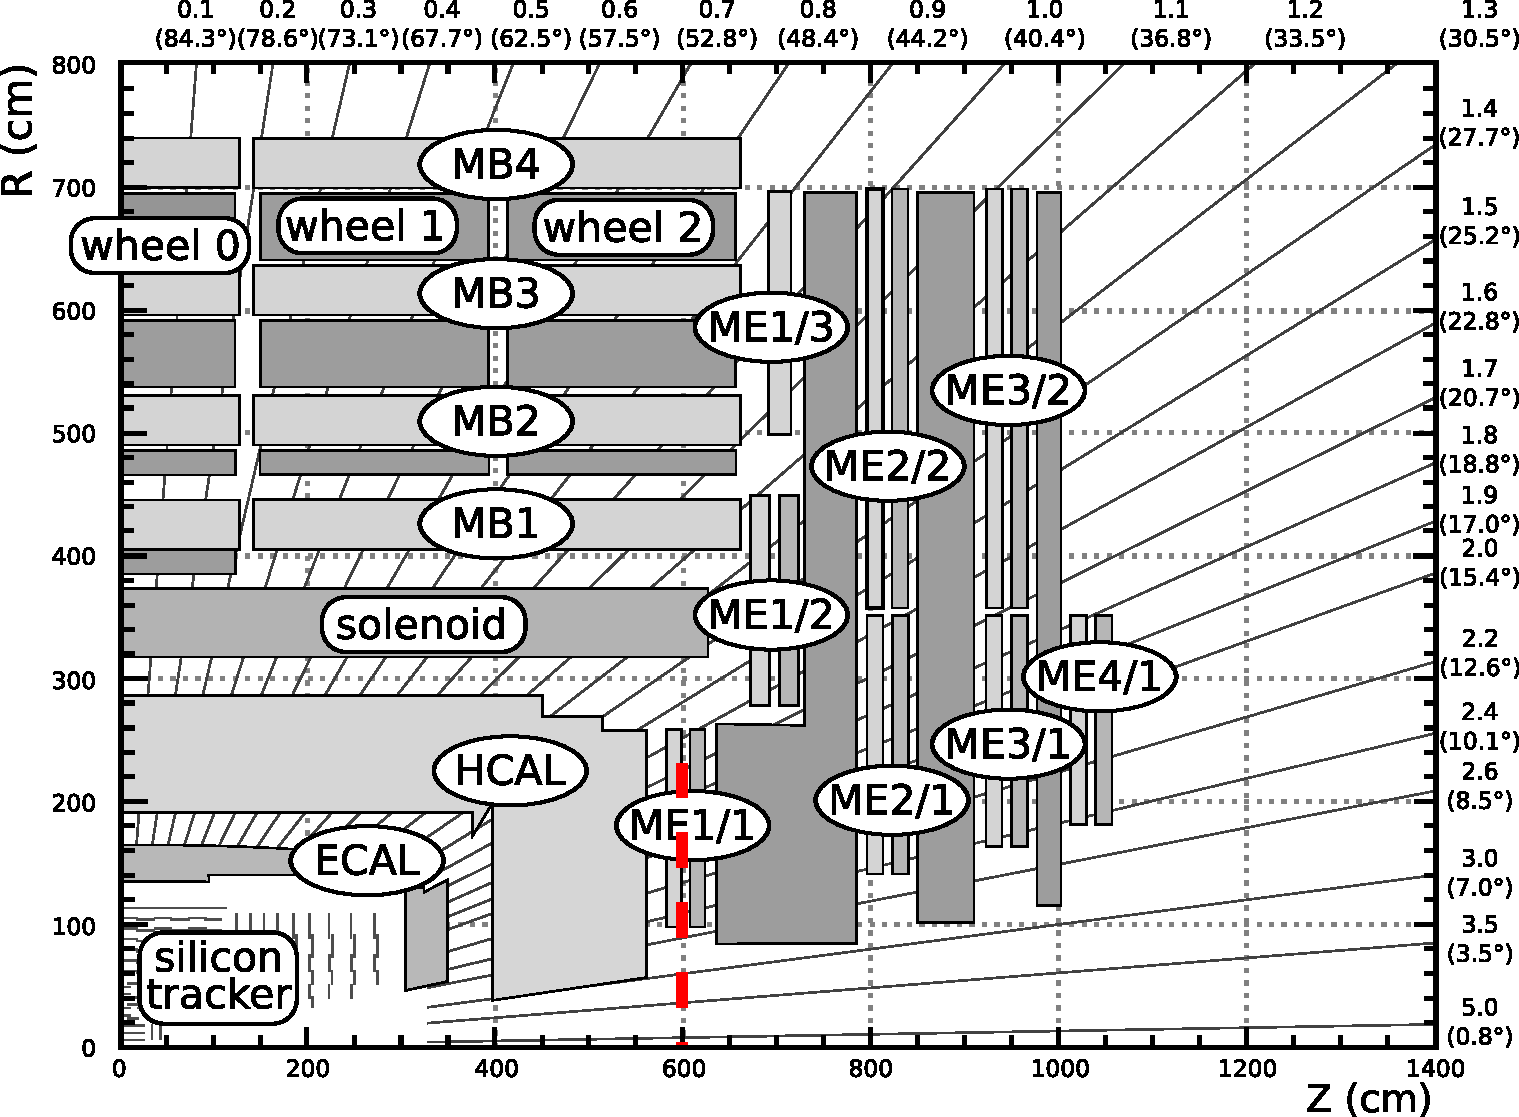
\includegraphics[width=0.4\linewidth]{muon_system_labeled2_me11Max.pdf} \\ 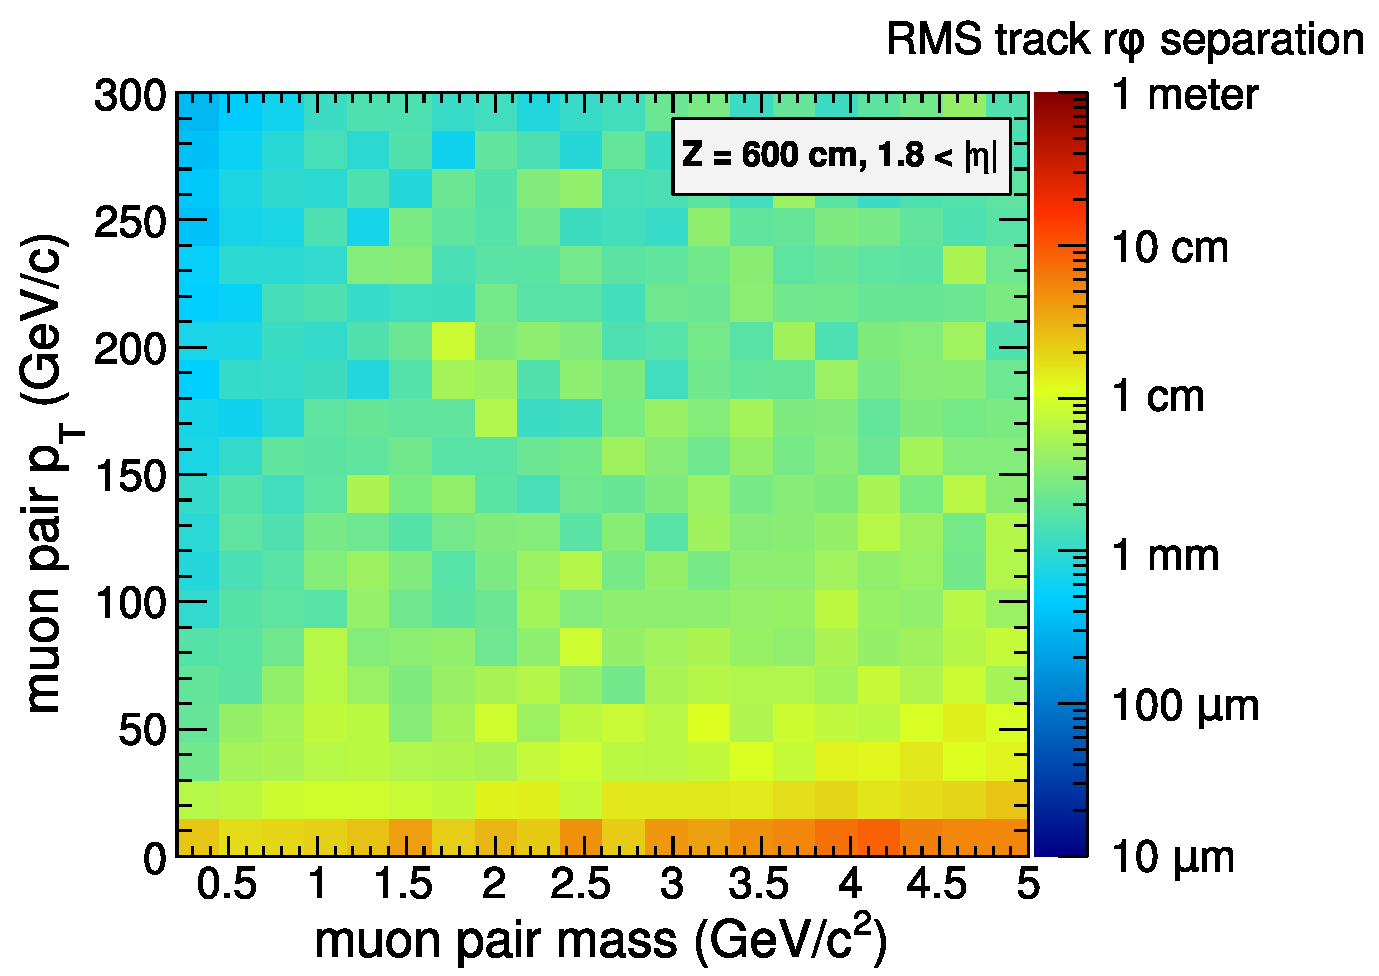
\includegraphics[width=0.7\linewidth]{openingangle_me11Max.pdf}}
\only<5>{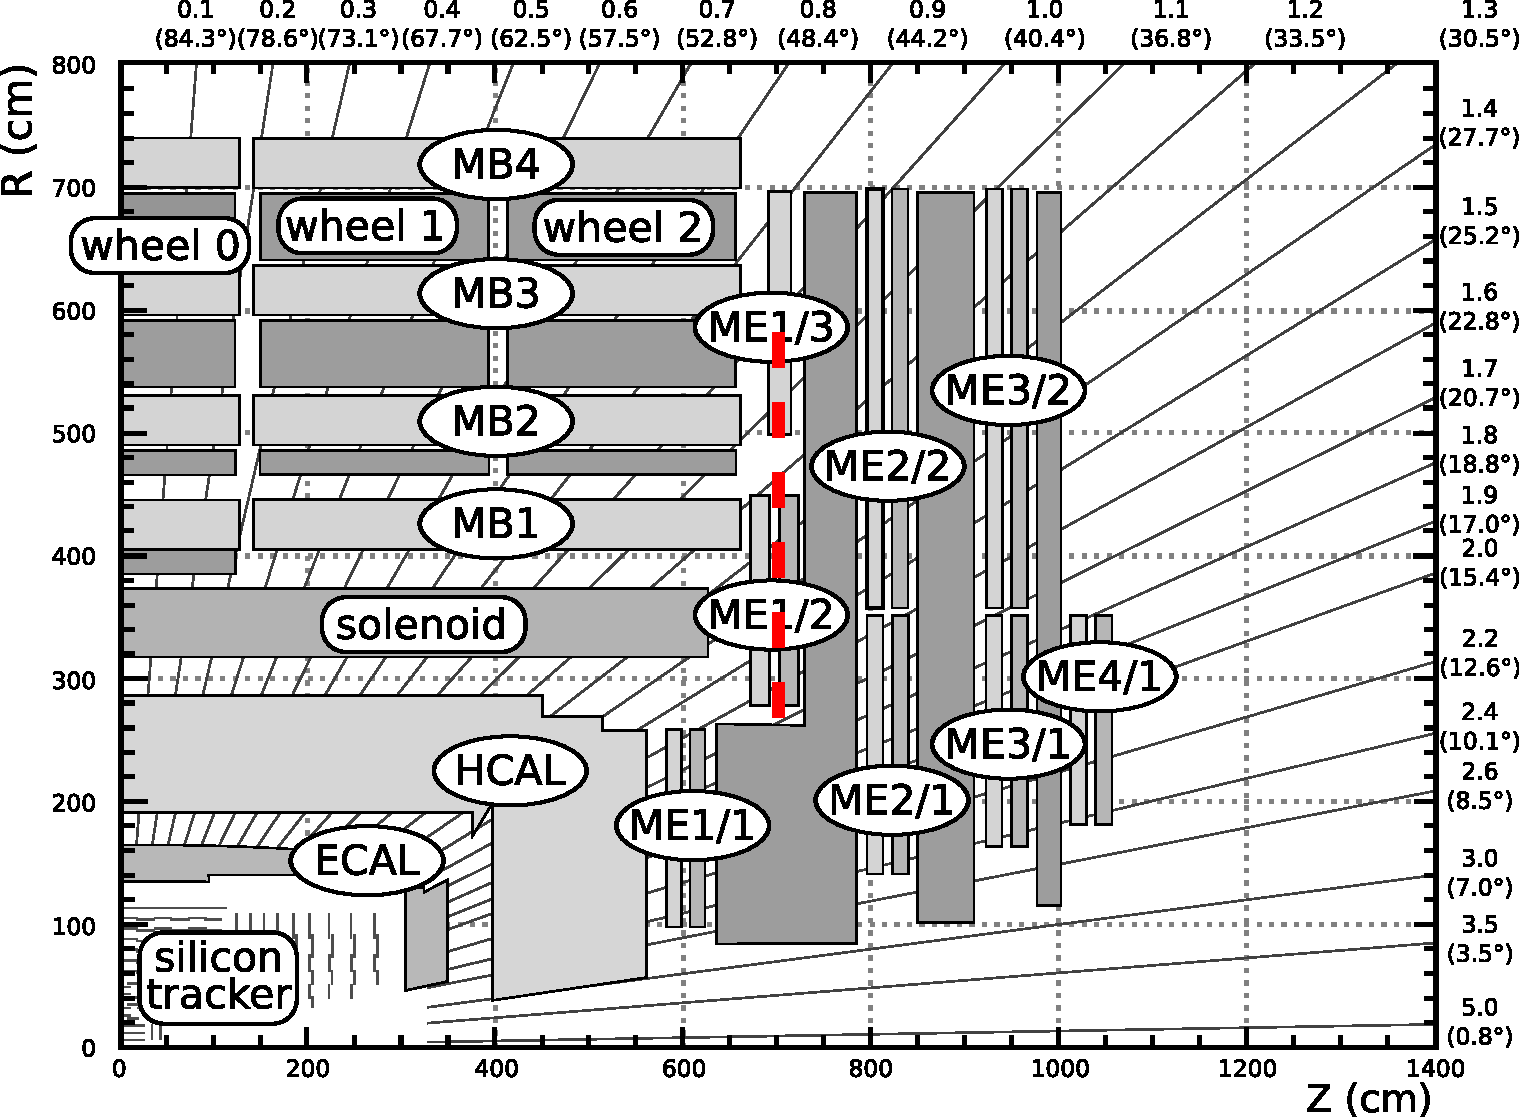
\includegraphics[width=0.4\linewidth]{muon_system_labeled2_me12Max.pdf} \\ 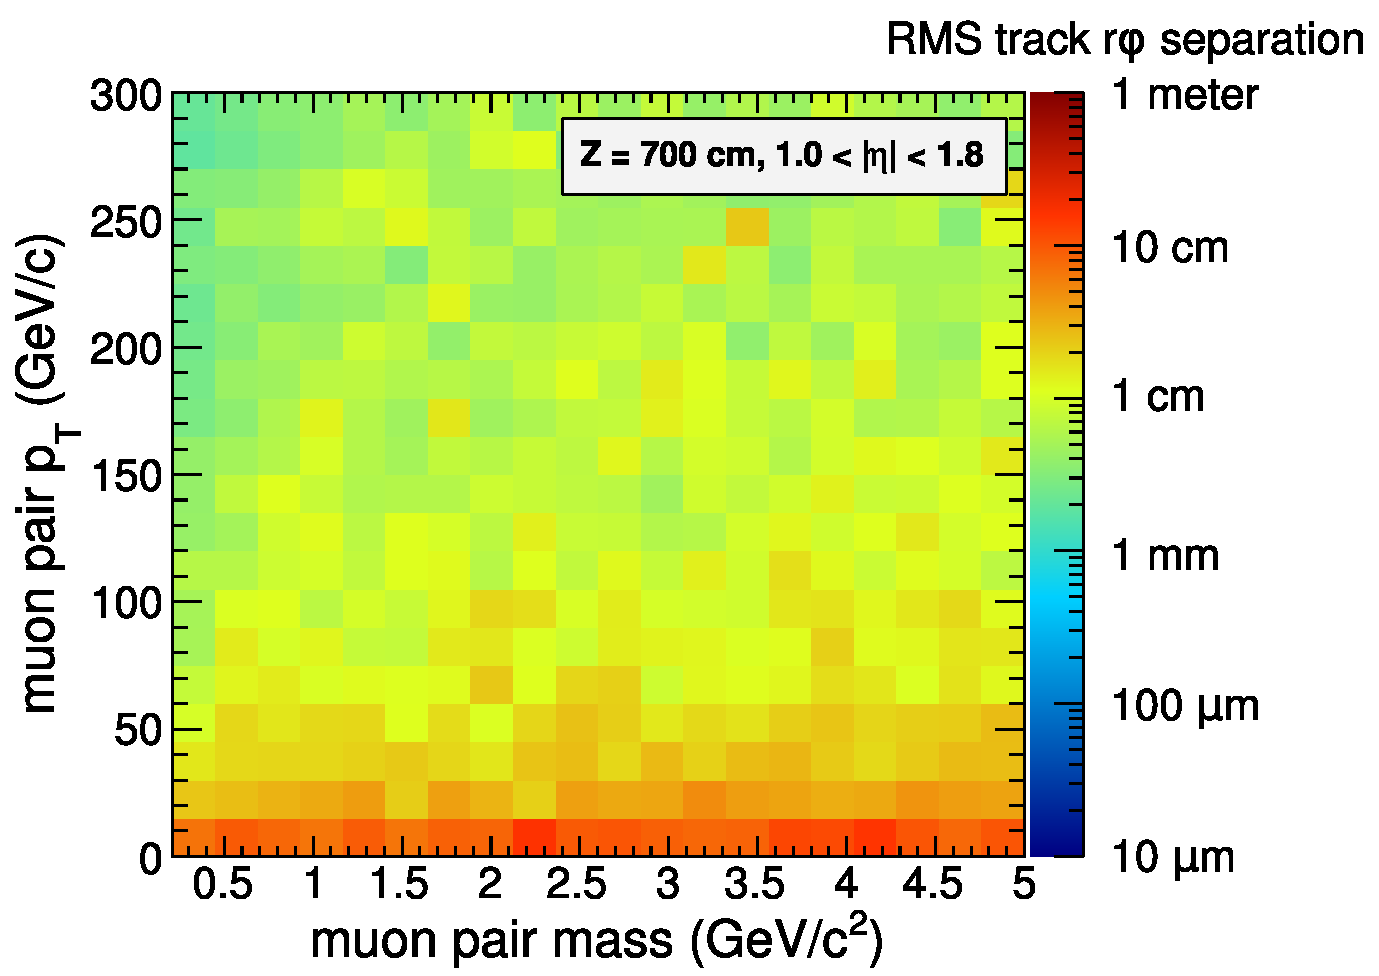
\includegraphics[width=0.7\linewidth]{openingangle_me12Max.pdf}}
\only<6>{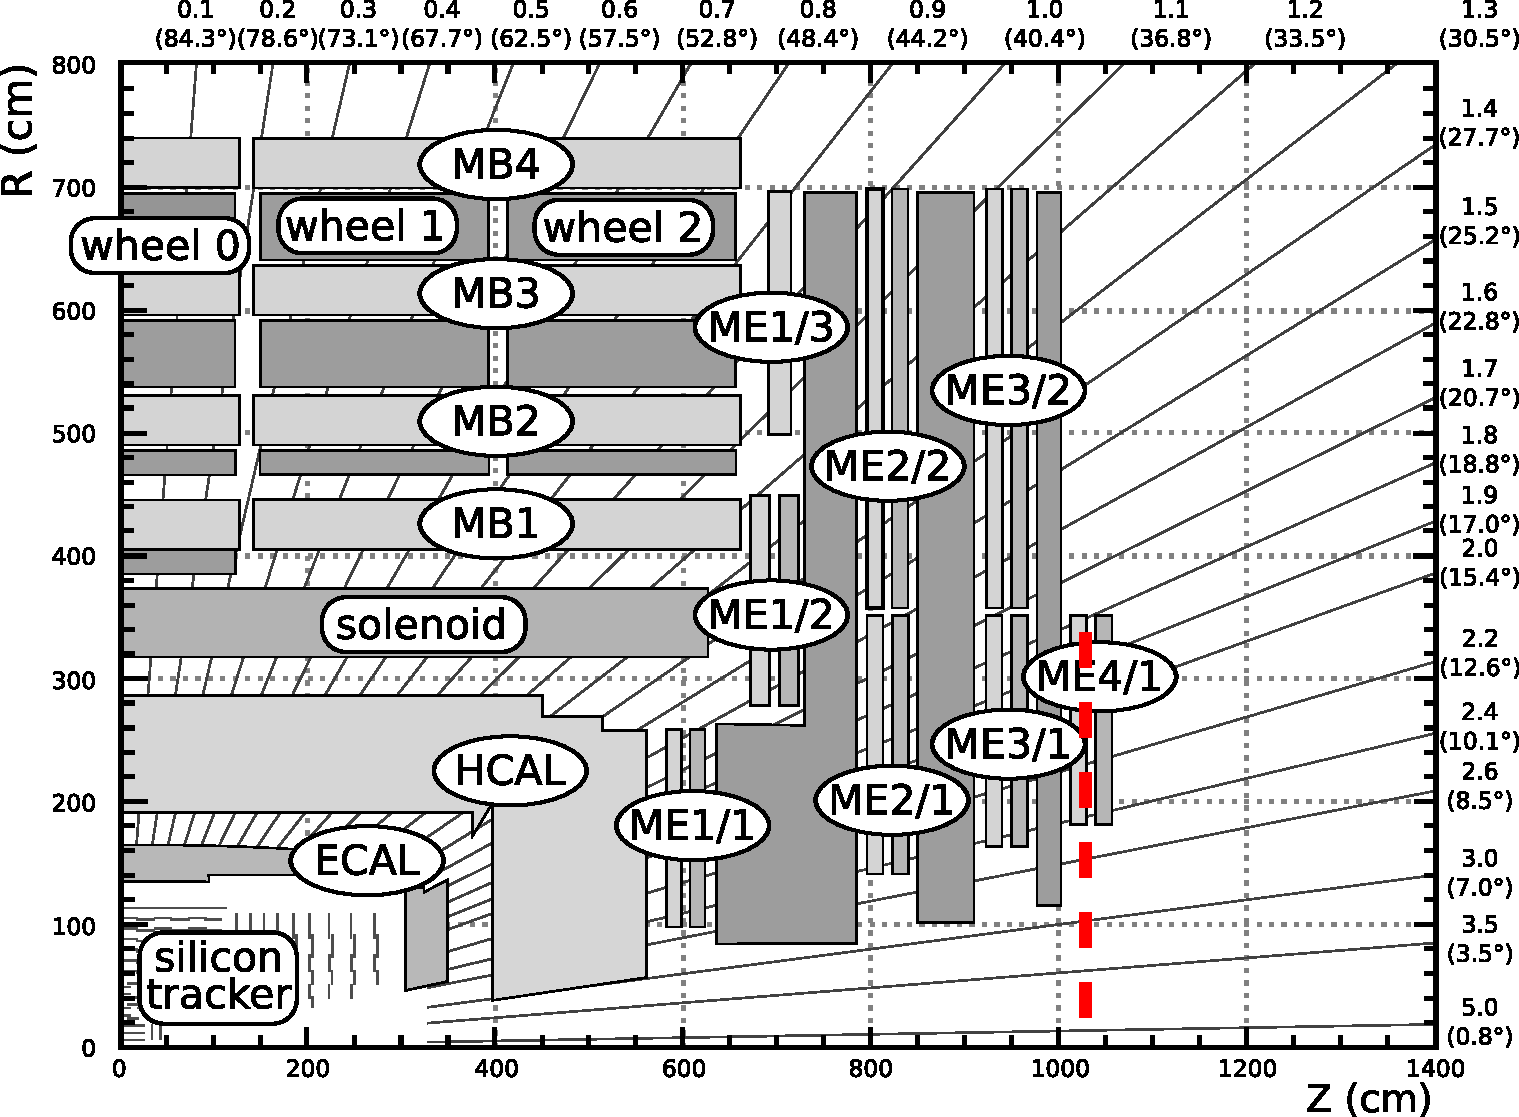
\includegraphics[width=0.4\linewidth]{muon_system_labeled2_me41Max.pdf} \\ 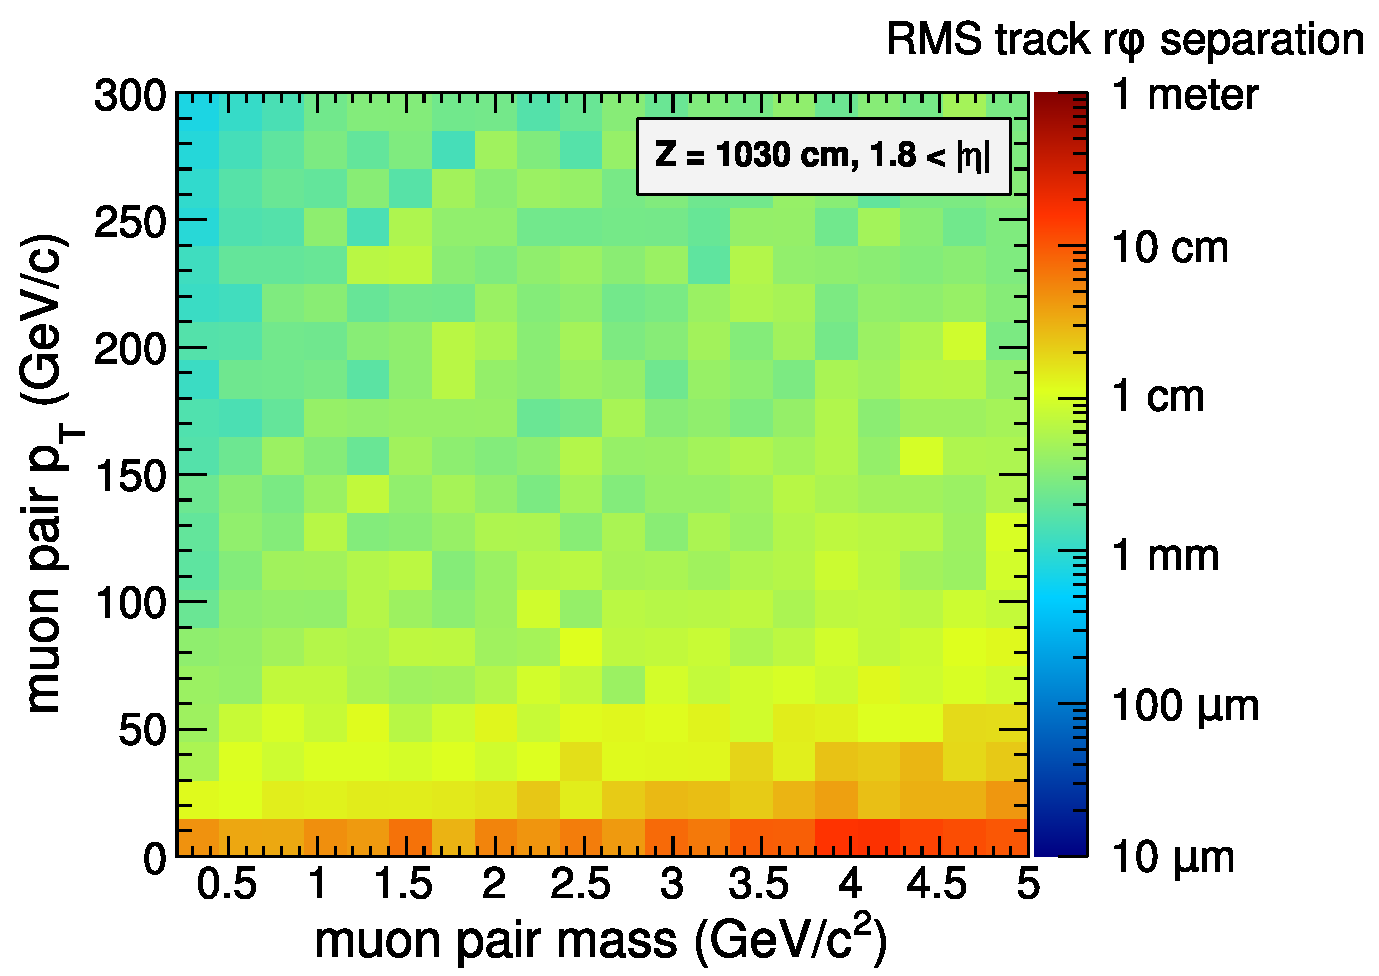
\includegraphics[width=0.7\linewidth]{openingangle_me41Max.pdf}}
\end{frame}

\end{document}

